\PassOptionsToPackage{utf8}{inputenc}
\documentclass{bioinfo}

\usepackage[]{algorithm2e}

\usepackage{booktabs}
\usepackage{rotating}

%%% for dags
\usepackage{tikz}
\usetikzlibrary{arrows}
\usetikzlibrary{fit,positioning, backgrounds}


\copyrightyear{2015} \pubyear{2015}

\access{Advance Access Publication Date: Day Month Year}
\appnotes{Manuscript Category}

\begin{document}
\firstpage{1}

\subtitle{Subject Section}

\title[Consensus clustering for Bayesian mixture models]{Consensus clustering for Bayesian mixture models}
\author[Sample \textit{et~al}.]{Stephen Coleman\,$^{\text{\sfb 1}*}$, Paul DW Kirk\,$^{\text{\sfb 1, \sfb 2}\dagger}$ and Chris Wallace\,$^{\text{\sfb 1,\sfb 2}\dagger}$}
\address{$^{\text{\sf 1}}$MRC Biostatistics Unit, University of Cambridge, Cambridge, CB2 0SR, United Kingdom and \\
$^{\text{\sf 2}}$Department of Medicine, University of Cambridge, Cambridge, CB2 0AW, United Kingdom.}

\corresp{$^\ast$To whom correspondence should be addressed. \newline $\dagger$ These authors provided an equal contribution.}

\history{Received on XXXXX; revised on XXXXX; accepted on XXXXX}

\editor{Associate Editor: XXXXXXX}

%\abstract{\textbf{Motivation:} 
%Ensemble  methods  have  been  highly  successful  in  many  applications. They frequently describe multiple feasible results with more ease than any individual learner.  ensemble methods may offer computational gains, using many independent, weak learners that may be run in parallel and thus faster than a comprehensive individual model. Bayesian mixture models are powerful and flexible tools for cluster analysis, enabling inference of the number of clusters present and modelling various data types through different choices of densities. However, inference is often performed using Markov-chain Monte Carlo methods which can suffer from problems, such as poor exploration of the posterior distribution and long runtimes, when applied ot high dimensional data. This makes applying Bayesian mixture models and their extensions to modern biomedical data a difficult matter. We apply the clustering ensemble method,consensus clustering, to Bayesian mixture models to address or sidestep problems with applying these methods to complex data.
%\textbf{Results:} 
%Consensus clustering of Bayesian mixture models finds generating structure in our simulation study. This approach successfully captures multiple modes in the likelihood surface and offers significant reductions in runtime when a parallel environment is available compared to use of a single long chain for traditional Bayesian inference. We propose a heuristic to decide upon the ensemble size and then apply consensus clustering to Multiple Dataset Integration, an extension of Bayesian mixture models for integra-tive analyses, on three ’omics datasets for the cell-cycle of budding yeast. We find clusters of genes that are co-expressed and have common regulatory proteins. These results show that consensus clusteringcan also be applied to more complex extensions of mixture models.
%}

\abstract{\textbf{Motivation:} 
Cluster analysis is an integral part of precision medicine and systems biology, used to define groups of patients or biomolecules, as well as more general analyses and data exploration. However, problems such as choosing the number of clusters and issues with high dimensional data arise consistently. An ensemble approach, such as consensus clustering, can overcome some of the difficulties associated with high dimensional data, frequently exploring more relevant clustering solutions than individual models. Another tool for cluster analysis, Bayesian mixture modelling, has alternative advantages, including the ability to infer the number of clusters present and extensibility. 
%modelling various data types through different choices of densities.
However, inference of these models is often performed using Markov-chain Monte Carlo (MCMC) methods which can suffer from problems, such as poor exploration of the posterior distribution and long runtimes, when applied to high dimensional data. This makes applying Bayesian mixture models and their extensions to 'omics data challenging. We apply the clustering ensemble method, consensus clustering, to Bayesian mixture models to address these problems from clustering complex data.\\ % and are severely under-utilised within ensembles. \\
% Bayesian mixture models have attractive features and been successfully applied in a diverse range of settings. Inference of these models is normally performed using Markov-chain Monte Carlo (MCMC) methods. In high dimensions MCMC methods often explore a limited range of partitions, with a lack of overlap between chains (i.e. a lack of convergence) frequently present.\\
\textbf{Results:} 
%We investigate the performance of this approach in simulations, comparing it to Bayesian inference of the same models and \texttt{Mclust}, a popular implementation of MLE inference of mixture models in R. 
Consensus clustering of Bayesian mixture models successfully finds generating structure in our simulation study. This approach successfully captures multiple modes in the likelihood surface and offers significant reductions in runtime when a parallel environment is available compared to use of a single long chain for traditional Bayesian inference. We propose a heuristic to decide upon the ensemble size and then apply consensus clustering to Multiple Dataset Integration, an extension of Bayesian mixture models for integrative analyses, on three 'omics datasets for the cell-cycle of budding yeast. We find clusters of genes that are co-expressed and have common regulatory proteins which we validate using external knowledge. Consensus clustering can be any MCMC-based clustering method and offers improvements in runtime in a parallel environment and better exploration of clustering space. \\
% compare this to inference performed using MCMC methods and also to \texttt{mclust}, a popular mixture model R package. We show that CC can be extended to Bayesian integrative clustering models. CC is then demonstrated on real datasets in both the single dataset and multiple dataset context. CC is shown to capture more modes in the clustering distribution than either the maximum-likelihood estimate (MLE) or any individual Markov chain. CC also reduces the computation time required when a parallel environment is present compared to Bayesian inference. \\
%\textbf{Availability:} www.github.com/stcolema/ccbm \\
\textbf{Contact:} \href{stephen.coleman@mrc-bsu.cam.ac.uk}{stephen.coleman@mrc-bsu.cam.ac.uk}\\
\textbf{Supplementary information:} Supplementary data are available at \textit{Bioinformatics} online.}

\maketitle

\section{Introduction}

%\subsection{Why cluster?}
From defining a taxonomy of disease to creating molecular sets, grouping items can help us to understand and make decisions using complex biological data. For example, grouping patients based upon disease characteristics and personal omics data may allow the identification of more homogeneous subgroups, enabling stratified medicine approaches. Defining and studying molecular sets can improve our understanding of biological systems as these sets are more interpretable than their constituent members \citep{hejblum2015time}, and study of their interactions and perturbations may have ramifications for diagnosis and drug targets \citep{bai2013strategic, emmert2014gene}. 

%allows the reaction and progression of individuals within a cluster to inform treatment decisions about other members of the same group. 


%Clustering data is about maximising the quantity of relevant data for each individual within a specific analysis, reducing from the complexity of the entire set without contracting to the individual level. The clustering approximates complex variation within the dataset, enabling local downstream analysis and decisions upon each group rather than at the global level. 

%\subsection{Why model-based clustering?}
The act of identifying such groups is referred to as “cluster analysis”. Traditional methods such as $K$-means clustering \citep{lloyd1982least, forgy1965cluster} or hierarchical clustering condition upon a user inputted choice of $K$, the number of occupied clusters present.  These methods are often heuristic in nature, relying on rules of thumb to decide upon a final model choice. For example, different choices of $K$ are compared under some metric such as silhouette or the within-cluster sum of squared errors (\textbf{SSE}) as a function of $K$. For $K$-means clustering, its sensitivity to initialisation means multiple runs are often used in practice, with that which minimises SSE used \citep{arthur2006k}. This problem arises as the algorithm has no guarantees on finding the global minimum of SSE.

%\subsection{Why Bayesian models?}
In many analyses or decision-making processes, quantifying confidence in the clustering can be of interest. Returning to the stratified medicine example of clustering patients, there might be individuals with almost equal probability of being allocated between several clusters which might influence decisions made.
%Knowing which individuals have uncertain membership could strongly influence decisions about treatment. 
However, many clustering algorithms provide only a point clustering.
% and thus one is no wiser about which individuals are boundary members of clusters. 

Ensemble methods offer a solution to the problems of sensitivity to initialisation and the lack of measure of uncertainty. These approaches have had great success in supervised learning, most famously in the form of Random Forest \citep{breiman2001random} and boosting \citep{friedman2002stochastic}. In clustering, consensus clustering \citep{monti2003consensus} is a popular method which has been implemented in R \citep{wilkerson2010consensusclusterplus, gu2020cola} and been applied to problems such as cancer subtyping \citep{lehmann2011identification, verhaak2010integrated} and identifying subclones in single cell analysis \citep{kiselev2017sc3}. Consensus clustering uses $W$ runs of some base model or learner (such as $K$-means clustering) and compiles the $W$ proposed partitions into a \emph{consensus matrix}, the $(i, j)^{th}$ entries of which contain the proportion of model runs for which the $i^{th}$ and $j^{th}$ individuals co-cluster (for this and other definitions see section 1 of the Supplementary Material). This proportion represents some measure of confidence in the co-clustering of any pair of items. Furthermore, ensembles can offer reductions in computational runtime. This is as the individual learners can be weaker (and thus use either less of the available data or stop before full convergence) and because the learners in most ensemble methods are independent of each other and thus enable use of a parallel environment for each of the quicker model runs \citep{ghaemi2009survey}. 

%Rather than using one model, an \emph{ensemble} can be used. Ensembles are often better able to explore the full parameter space than any individual learner in its composition, thus describing more modes within parameters than the individual learners \citep{ghaemi2011review}. Ensembles also offer reductions in computational runtime because most ensemble methods enable use of a parallel environment to improve computation speed \citep{ghaemi2009survey}. Consensus clustering \citep{monti2003consensus} is an ensemble method for cluster analysis, previously applied using a base learner of $K$-means clustering in the R package \texttt{ConsensusClusterPlus} \citep{wilkerson2010consensusclusterplus}. This flavour of consensus clustering has been applied to cancer subtyping \citep{lehmann2011identification, verhaak2010integrated} and identifying subclones in single cell analysis \citep{kiselev2017sc3}. The algorithm applies $R$ independent runs of the base model to perturbed versions of the dataset and combines the $R$ final partitions in a \emph{consensus matrix} (CM) to infer a final clustering. The consensus matrix is a symmetric matrix with the $(i, j)^{th}$ entry being the proportions of model runs for which the $i^{th}$ and $j^{th}$ items are clustered together. For a single partition the \emph{coclustering matrix} represents this information, being a binary matrix with the $(i, j)^{th}$ entry indicating if items $i$ and $j$ are allocated to the same cluster.

\cite{monti2003consensus} proposed some methods for choosing $K$ using the consensus matrix, but this remains a problem in the methods mentioned so far. An alternative clustering framework, model-based clustering or \emph{mixture models}, embeds the cluster analysis within a formal, statistical framework \citep{fraley2002model}. This means that models can be compared formally, and problems such as the choice of $K$ can be addressed as a model selection problem with all the associated tools. Mixture models are also attractive, as they have great flexibility in the type of data they can be applied to due to different choice of densities.

Furthermore, \emph{Bayesian mixture models} can treat $K$ as a random variable that is inferred from the data and thus the final clustering is not conditional upon a user chosen value, but $K$ is jointly modelled along with the clustering. Such inference can be performed through use of a Dirichlet Process \citep{ferguson1973bayesian}, a mixture of finite mixture models \citep{richardson1997bayesian, miller2018mixture} or an over-fitted mixture model \citep{rousseau2011asymptotic, van2015overfitting}. These models and their extensions have a history of successful application to a diverse range of biological problems such as finding clusters of gene expression profiles \citep{medvedovic2002bayesian}, cell types in flow cytometry \citep{chan2008statistical, hejblum2019sequential} or scRNAseq experiments \citep{prabhakaran2016dirichlet}, and estimating protein localisation \citep{crook2018bayesian}. Bayesian mixture models can be extended to jointly model the clustering across multiple datasets \citep{kirk2012bayesian, gabasova2017clusternomics}. More details of Bayesian mixture models and an example of an extension to an integrative setting can be found in section 2 of the Supplementary Material.

%The most common models where $K$ is inferred are the mixture of finite mixtures (\citealp{miller2018mixture}, frequently implemented using Reversible Jump MCMC moves via \citealp{richardson1997bayesian}), the Dirichlet process \citep{ferguson1973bayesian, neal2000markov} or the overfitted mixture model \citep{van2015overfitting}.

% provide an uncertainty quantification that allows one to include this uncertainty in a formal manner in downstream analyses and decisions. These models and their extensions have a history of successful application to a diverse range of biological problems such as finding clusters of gene expression profiles \citep{medvedovic2002bayesian}, cell types in flow cytometry \citep{chan2008statistical, hejblum2019sequential} or scRNAseq experiments \citep{prabhakaran2016dirichlet}, and estimating protein localisation \citep{crook2018bayesian}.

%One might believe that the number of occupied clusters present, $K$, is a random variable that should be inferred from the data. Bayesian mixture models can treat $K$ in this way, thereby incorporating uncertainty about $K$ into the the allocation uncertainty and reducing some of the subjectivity of choosing $K$. The most common models for are the mixture of finite mixtures (\citealp{miller2018mixture}, frequently implemented using Reversible Jump MCMC moves via \citealp{richardson1997bayesian}), the Dirichlet process \citep{ferguson1973bayesian, neal2000markov} or the overfitted mixture model \citep{van2015overfitting}. In these models the number of components and the component parameters are modelled jointly, in contrast with many clustering methods. Furthermore, if there is a prior information about $K$, this may be included due to the Bayesian nature of the model. 
%
%We write the basic mixture model for independent items $X=(x_1, \ldots, x_N)$ as 
%\begin{align}
%x_i \sim \sum_{k=1}^K\pi_k f(x_i | \theta_k) \hspace{1cm} \textrm{independently for $i = 1,\ldots,N$}
%\end{align}
%where $f(\cdot| \theta)$ is some family of densities parametrised by $\theta$. A common choice is the Gaussian density function, with $\theta=(\mu, \sigma^2)$. $K$, the number of subgroups in the population, $\{\theta_k\}_{k=1}^K$, the component parameters, and $\pi=(\pi_1, \ldots, \pi_K)$, the component weights are the objects to be inferred. In the context of \emph{clustering}, such a model arises due to the belief that the population from which the random sample under analysis has been drawn consists of $K$ unknown groups proportional to $\pi$. In this setting it is natural to include a latent \emph{allocation variable}, $c=(c_1, \ldots, c_N)$, to indicate which group each item is drawn from. The model is then
%\begin{equation}
%	\label{eqn:mixModel}
%	\begin{array}{r@{}l l}
%		p(c_i = k) = \pi_k&  &\textrm{for $k = 1,\ldots,K$,} \\
%		x_i | c_i \sim f(x_i | \theta_k)& &\textrm{independently for $i = 1,\ldots,N$.} 
%	\end{array}
%\end{equation}
%The joint model can then be written
%\begin{align}
%	p(X, c, K, \pi, \theta) &= p(X | c, \pi, K, \theta) p(\theta | c, \pi, K) p(c | \pi, K) p(\pi | K) p(K) \nonumber
%\end{align}
%An assumption that is frequently used is that the density of each feature is independent, with $\theta_k=(\theta_{k1},\ldots, \theta_{kP})$ for all $k=1,\ldots,K$. Furthermore, conditional independence is assumed between certain parameters such that the model reduces to
%
%\begin{align}
%	p(X, c, \theta, \pi, K) &=  p(\pi | K) p(\theta | K) p(K) \prod_{i=1}^N p(x_i | c_i, \theta_{c_i}) p (c_i | \pi, K).  \label{eqn:jointMixModel}
%%	\\
%%	&= \prod_{i=1}^N \prod_{p=1}^P p(x_{ip} | c_i, \theta_{c_ip})^{(1 - \phi_p)} p(x_{ip} | \theta_p) ^ {\phi_p} \times \\
%%	& \prod_{i=1}^N p (c_i | \pi, K) p(\pi | K) p(\theta | K)
%\end{align}
%
%Bayesian mixture models have been extended to the multiple dataset context where they are used to perform integrative clustering. This means that as much pertinent information as possible can be included in the joint model. Multiple Dataset Integration \citep[\textbf{MDI}, ][]{kirk2012bayesian} is an example of such a model where dataset specific clusterings are learnt, informed by common information. This is captured by the different prior on the allocation
%\begin{align}
%	p(c_{n1}, \ldots, c_{nL}) \propto \prod_{l=1}^L \pi_{c_{nl}l}\prod_{i=1}^{L-1}\prod_{j=i+1}^L(1 + \phi_{ij} \mathbb{I}(c_{ni} = c_{nj}))
%	\label{eqn:mdiPrior}
%\end{align}
%for $L$ datasets and $n = 1,\ldots, N$. $\phi_{ij}$ is the parameter defined by the correlation of the clusterings for the $i^{th}$ and $j^{th}$ datasets. As this increases more mass is placed on the common partition for $i$ and $j$. Conversely, as $\phi_{ij}\to 0$ we have independent mixture models. In this way the correlation of the clustering between each pair of datasets controls how information is shared across each clustering, with more correlated datasets influencing each other and uncorrelated datasets remaining independent.



%\begin{align}
%	
%	&p(c_i = k) = \pi_k&  \textrm{for $k = 1,\ldots,K$,} \nonumber\\
%	&x_i | c_i \sim f(x_i | \theta_k)& \textrm{independently for $i = 1,\ldots,N$.} \nonumber
%\end{align}

%Visualisations of different embeddings of the data (such as Principal Component Analysis \cite{wold1987principal} or non-linear methods such as t-stochastic neighbourhood embedding \cite{maaten2008visualizing} or Poincaré maps \cite{klimovskaia2020poincare}) might offer some beliefs about the $K$.

%The uncertainty in the clustering is conditioned upon this fixed $K$. Unless the number of subpopulations present is truly known (a rare occasion), treating $K$ as a random variable to be inferred from the data is attractive. This both reduces the subjectivity of the user choice and also incorporates more of the true uncertainty present into the clustering. Bayesian mixture models do allow this, and also enable inclusion of prior belief about the number of clusters present. 


%it can be difficult or even impossible to have a strong opinion on this a priori, particularly with the high-dimensional datasets that arise from modern ‘omics technologies. Non-linear dimension reduction algorithms such as t-distributed stochastic neighbour embedding (t-SNE), uniform manifold approximation and projection (UMAP) and Poincaré maps allow visualisation that may provide some intuition about the structure present; however these compressed representations should not be interpreted too deeply and thus the ``true'' number of clusters present remains an elusive quantity.


%Inferring the membership of these groups and the number of such groups present is a difficult problem, as  Traditional clustering algorithms (e.g. $K$-means clustering, hierarchical clustering) condition upon a fixed, user selected value for the number of clusters to identify. However, excluding the uncertainty about this parameter, $K$, under-estimates the uncertainty on the membership of many items. Inferring this quantity from the data and treating it as a random variable with uncertainty is therefore attractive as it removes the subjective prior choice of $K$ and includes more of the uncertainty present. 




%Cluster analysis is used to uncover interesting, separate groups within data. $K$ homogeneous clusters are constructed from a dataset of $N$ items, with $K << N$ (normally). This offers insights into structure within the data, as interpreting $K$ homogeneous clusters is easier than considering the $N$ items in the original dataset. This structure may be itself of interest, or else used as a pre-processing step to create cluster-specific models. As the cluster analysis approximates variation within the data, the combination of this with local models can describe complex, non-linear behaviour in a relatively interpretable model \cite{gadd2020enriched}.

%Within biomedical analyses, cluster analysis has had many specific contributions ranging from subtyping of complex diseases and classification of patients in precision medicine to constructing gene sets and contributing to drug-target prediction. 

%Model-based clustering embeds cluster analysis within a rigorous statistical framework that offers clear rules on model comparison \cite{fraley2002model}. This reduces the degree of subjectivity present in cluster analysis as questions such as choice of $K$ (an input in many clustering algorithms) is turned into a model comparison question. 

%Bayesian mixture models specifically are attractive. These enable:
%\begin{itemize}
%	\item inclusion of a prior distribution on parameters enables researchers to represent existing knowledge in a model.
%	\item inference of $K$, the number of occupied clusters \cite{ferguson1973bayesian}.
%	\item formal quantification of uncertainty.
%\end{itemize}

%\subsection{Problem}
Inference may be performed upon Bayesian mixture models using variational inference \citep[\textbf{VI},][]{blei2006variational}.
% or the sequential updating and greedy search \citep[\textbf{SUGS},][]{wang2011fast, zhang2014sequential, crook2019fast}.
While VI is powerful, ``it is not yet well understood'' \citep{blei2017variational}. Furthermore, VI can struggle with multi-modality, underestimates the variance in the posterior distribution \citep{two2011turner} and it has been shown to have a very computationally heavy initialisation cost to have good results \citep{wang2011fast}. Implementation is difficult, requiring either complex derivations \citep[see the Appendix Supplementary Methods of][for an example]{argelaguet2018multi} or black-box, approximate solutions \citep{kucukelbir2017automatic}.

However, Markov chain Monte Carlo (MCMC) methods are the most popularly method for Bayesian inference. In Bayesian clustering methods, MCMC methods are used to construct a chain of clusterings, and then an assessment of the convergence of this chain is made, to determine if its behaviour aligns with the expected asymptotic theory. This chain of samples will converge to the posterior distribution of the Bayesian model and explore its entire support given an infinite runtime. However, in practice problems arise. Individual chains often fail to explore the full support of the posterior distribution \citep[an example of different chains becoming trapped in a single mode of the likelihood surface can be seen in the Supplementary Materials of ][]{strauss2020gpseudoclust} and experience slow runtimes. Some MCMC methods make efforts to overcome the problem of exploration, often at the cost of increased computational cost per iteration. For a description of some of the problems and attempted solutions for MCMC methods, both generally and in clustering, see \cite{robert2018accelerating, yao2020stacking, chandra2020bayesian}. 

We propose that applying consensus clustering to Bayesian mixture models can overcome some of the issues endemic in high dimensional Bayesian clustering. \cite{monti2003consensus} suggest this application as part of their original paper, but no investigation has been attempted to our knowledge. This ensemble approach  sidesteps the problems of convergence associated MCMC methods and offers computational gains through using shorter chains run in parallel. Furthermore, this approach could be directly used on any existing MCMC based implementation of Bayesian mixture models or their extensions and would avoid the re-implementation process that changing to newer MCMC methods or VI would entail.

We propose a heuristic for deciding upon the ensemble width (the number of learners used, $W$) and the ensemble depth (the number of iterations run within each chain, $D$), inspired by the use of scree plots in Principal Component Analysis \citep[\textbf{PCA}][]{wold1987principal}.


We show via simulation that ensembles consisting of short chains can be sufficient to successfully recover generating structure. We also show that consensus clustering explores as many or more modes of the likelihood surface than either standard Bayesian inference or \texttt{Mclust}, a maximum likelihood method, all while offering improvements in runtime to traditional Bayesian inference.
%in a number of scenarios including some within which a single chain becomes trapped in individual modes of the likelihood surface for any reasonable length of runtime. The chains are relatively short and independent, thus their individual runtime is far shorter than the chains traditionally used for Bayesian inference and also may be run in parallel. This means that consensus clustering of Bayesian mixture models offers significant reductions in runtime. We also show that the ensemble can describe multiple modes in scenarios where any individual chain becomes trapped, and thus the uncertainty present in the consensus matrix can be more representative of the data. Within the same simulated data we compare consensus clustering to standard Bayesian analysis with long chains, and a maximum likelihood method, \texttt{Mclust}.

%Based upon the behaviour of consensus clustering within the simulated data 
%We then perform an integrative analysis of 'omics data relating to the cell cycle of \emph{Saccharomyces cerevisiae}. 

We go on to perform an integrative analysis of cell cycle data from \emph{Saccharomyces cerevisiae}. The cell cycle is the process by which a growing cell divides into two daughter cells. This involves virtually all cellular processes 
%- metabolism, protein synthesis, secretion, DNA replication, organelle biogenesis, cytoskeletal dynamics and chromosome segregation - 
and diverse regulatory events \citep{granovskaia2010high}. The cell cycle is crucial to biological growth, repair, reproduction, and development
%; it is fundamental to sustaining life 
\citep{tyson2013cell, chen2004integrative, alberts2018molecular}. The regulatory proteins of the 
%system first appeared over a billion years ago and are
cell cycle are so highly conserved among eukaryotes that many of them function perfectly when transferred from a human cell to a yeast cell \citep{alberts2018molecular}. This conservation means that a relatively simple eukaryote such as \emph{Saccharomyces cerevisiae} can provide insight into a variety of cell cycle perturbations including those that occur in human cancer \citep{ingalls2007systems, chen2004integrative} and ageing \citep{jimenez2015live}. Budding yeast is particularly attractive for genetic analysis as
%it can proliferate as haploid cells, its genetic makeup can be easily altered by standard tools of molecular genetics \citep{tyson2013cell}, and 
large numbers of cells may be synchronised in a particular stage of the cell cycle  \citep{juanes2017methods}. We apply consensus clustering to an extension of Bayesian mixture models, Multiple Dataset Integration (\textbf{MDI}), a multiple dataset clustering method. 
%Cluster analysis of a single 'omics dataset entails interpreting the clusters defined by similarity within a single experiment which often involves strong assumptions about the biological processes behind the result (e.g. correlation of transcripts implies co-regulation). However, by integrating multiple experiments we believe that the analysis is more interpretable, and the greater information modelled means that the cluster 
We determine the ensemble size using our proposed stopping rule. We use this ensemble to infer clusters of genes across datasets and validate these clusters using knowledge external to the analysis. 
% with similar expression across time with common regulatory proteins showing that consensus clustering of Bayesian mixture models can be used to perform meaningful, useful inference. 

%We show on three datasets from the original MDI paper that consensus clustering performs similarly to Bayesian inference of this model, and then using more modern, larger data that consensus clustering enables implementation of such models in scenarios where the problem of long runtimes and poor mixing previously discouraged this. 

%Bayesian inference for mixture models and their extensions is normally performed using Markov-chain Monte Carlo (MCMC). However, MCMC is known to display problematic behaviour in high-dimensions \citep{robert2018accelerating, yao2020stacking, chandra2020bayesian}. One of these problems is the difficulty in exploring a range of modes in the posterior distribution of the clustering. This leads to a lack of convergence across chains and the distribution in any single chain is highly concentrated upon a very small number (often one) possible clustering(s). Another problem that emerges in large or high-dimensional datasets is that individual iterations of the MCMC sampler become slow and a long chain can become infeasible.


%with the collapsed Gibbs sampler \cite{liu1994collapsed} being particularly prominent for mixture models as it enables integrating over nuisance parameters. An example of this is marginalising out the covariance matrix in a mixture of Gaussian models. This quantity is often the cause of singularities in the likelihood surface that cause the inference to fail, a common issue for MLE inference of mixture models.
%
%However, MCMC methods in general \cite{robert2018accelerating, yao2020stacking, chandra2020bayesian} and the collapsed Gibbs sampler in particular \cite{bishop2006pattern} are known to display problematic behaviour in high-dimensions . One of these problems is the difficulty in exploring a range of modes in the posterior distribution of the clustering. This means that there is a lack of convergence across chains and the distribution in any single chain is highly concentrated upon a very small number (often one) possible clustering(s).

%\subsection{Solution}
%\subsubsection{Ensembles}
%An alternative approach to clustering is through the use of ensembles of models. Ensembles are often better able to explore the full parameter space than any individual learner in its composition, thus describing more modes within parameters than the individual learners \citep{ghaemi2011review}. Ensembles also offer reductions in computational runtime because most ensemble methods enable use of a parallel environment to improve computation speed \citep{ghaemi2009survey}. Consensus clustering \citep{monti2003consensus} is an ensemble method for cluster analysis, previously implemented using $K$-means clustering in the R package \texttt{ConsensusClusterPlus} \citep{wilkerson2010consensusclusterplus}. This flavour of consensus clustering has been applied to cancer subtyping \citep{lehmann2011identification, verhaak2010integrated} and identifying subclones in single cell analysis \citep{kiselev2017sc3}. Consensus clustering applies $D$ independent runs of the clustering algorithm to peturbed versions of the dataset and combines the $D$ final partitions in a \emph{consensus matrix} (CM) to infer a final clustering. The consensus matrix is a symmetric matrix with the $(i, j)^{th}$ entry being the proportions of model runs for which the $i^{th}$ and $j^{th}$ items are clustered together. For a single partition the \emph{coclustering matrix} represents this information, being a binary matrix with the $(i, j)^{th}$ entry indicating if items $i$ and $j$ are allocated to the same cluster.


%definition CM

%\begin{algorithm} \label{algorithm:CC}
%	\KwData{\(X=(x_1, \ldots, x_N)\)}
%	\KwIn{A resampling scheme \emph{Resample} \\ A clustering algorithm \emph{Cluster} \\ Number of resampling iterations $W$ \\ Set of cluster numbers to try $\mathcal{K}=\{K_1, \ldots, K_{max}\}$}
%	\KwOut{A predicted clustering, $\hat{Y}$ \\ The predicted number of clusters present $\hat{K}$}
%	%	\KwResult{how to write algorithm with \LaTeX2e }
%	\Begin{
%		\For{$K \in \mathcal{K}$}{
%			\tcc{initialise an empty consensus matrix}
%			$\mathbf{M}^{(K)} \leftarrow \mathbf{0}_{N \times N}$\;
%			\For{$w = 1$ \KwTo $W$}{
%				$X^{(s)} \leftarrow Resample(X)$\;
%				
%				\tcc{Cluster the peturbed dataset, represented in a coclustering matrix}
%				$\mathbf{B}^{(s)} \leftarrow Cluster(X^{(s)}, K)$\;
%				$\mathbf{M}^{(K)} \leftarrow \mathbf{M}^{(K)} + \mathbf{B}^{(s)}$\;
%			}
%			$\mathbf{M}^{(K)} \leftarrow \frac{1}{W} \mathbf{M}^{(K)}$\;
%		}
%		$\hat{K} \leftarrow$ best $K \in \mathcal{K}$ based upon all $\mathbf{M}^{(K)}$\;
%		$\hat{Y} \leftarrow$ partition $X$ based upon $\mathbf{M}^{(\hat{K})}$\;
%	}
%	\caption{Consensus clustering algorithm. \cite{monti2003consensus} suggest rules for both choosing the best $K \in \mathcal{K}$ and for inferring a point estimate clustering from $\mathbf{M}^{(\hat{K})}$. $\mathbf{B}^{(s)}$ is the co-clustering matrix for the $s^{th}$ model run.}
%\end{algorithm}

%\subsubsection{Consensus clustering of Bayesian mixture models}
%We adapt consensus clustering to Bayesian mixture models. We show via simulation that ensembles consisting of short chains are sufficient to uncover meaningful structure in a number of scenarios including some within which a Gibbs sampler becomes trapped in individual modes for any reasonable length of runtime. The chains are both short and independent, thus their individual runtime is far shorter than the chains traditionally used for Bayesian inference and may also be run in parallel. This means that consensus clustering of Bayesian mixture models offers significant reductions in runtime without sacrifices in performance. As the ensemble can describe multiple modes, the uncertainty present in the consensus matrix can be more representative of the data than the individual modes captured by any single chain.

%We then apply our algorithm to the multiple dataset setting and the extension of Bayesian mixture models, Multiple Dataset Integration (MDI). We show on three datasets from the original MDI paper that consensus clustering performs similarly to Bayesian inference of this model, and then using more modern, larger data that consensus clustering enables implementation of such models in scenarios where the problem of long runtimes and poor mixing previously discouraged this. 

%\enlargethispage{12pt}

%\begin{methods}
%\section{Methods}

%\subsection{Mixture models}
%We write the basic mixture model for independent items $X=(x_1, \ldots, x_N)$ as 
%\begin{align}
%	x_n \sim \sum_{k=1}^K\pi_k f(x_n | \theta_k) \hspace{1cm} \textrm{independently for $n = 1,\ldots,N$}
%\end{align}
%where $f(\cdot| \theta)$ is some family of densities parametrised by $\theta$, with each $f(\cdot| \theta)$ being a \emph{component} of the mixture model. A common choice is the Gaussian density function, with $\theta=(\mu, \sigma^2)$. $K$, the number of components modelled, $\{\theta_k\}_{k=1}^K$, the component parameters, and $\pi=(\pi_1, \ldots, \pi_K)$, the component weights are the objects to be inferred. In clustering, such a model arises due to the belief that the population from which the random sample under analysis has been drawn consists of $K$ unknown groups proportional to $\pi$, with each component describing one of these subpopulations. In this setting it is natural to include a latent \emph{allocation variable}, $c=(c_1, \ldots, c_N)$, to indicate which group each item is drawn from. As the number of sub-groups present in the sample may be less than that of the population, some components may have no allocated items. In this case each non-empty component of the mixture corresponds to a cluster. The model is
%\begin{equation}
%	\label{eqn:mixModel}
%	\begin{array}{r@{}l l}
%		p(c_n = k) = \pi_k&  &\textrm{for $k = 1,\ldots,K$,} \\
%		x_n | c_n \sim f(x_n | \theta_k)& &\textrm{independently for $n = 1,\ldots,N$.} 
%	\end{array}
%\end{equation}
%More details of the mixture model can be found in section 2.1 of the Supplementary Material.
%\subsection{\texttt{Mclust}}
%\texttt{Mclust} \citep{mclust2016scrucca} is a function that estimates and compares Gaussian mixture models based upon the maxmimum likelihood estimator of the parameters for a range of choices of $K$, the number of clusters used, and different covariance structures. The method initialises upon a hierarchical clustering of the data cut to $K$ clusters. The ``best'' model is determined using the Bayesian information criterion, \citep[\textbf{BIC},][]{schwarz1978estimating}.
%\end{methods}
%
%\subsection{Bayesian inference}
%%We use 10 long chains in where ``Bayesian inference'' is being considered in the simulations and the yeast analysis. In the simulations chains are kept in the analysis based upon a number of tests described below. To summarise the chains that are considered ``converged'' we pool the samples from across the chains (effectively using an ensemble of long chains). This choice is considered more in the supplementary materials. These pooled samples are expected to be an upper bound on the performance of any single chain in the simulations.
%
%
%%I think have this in supplementary,remove from here.
%The model we use is a mixture of \emph{Gaussian} distributions.
%% and thus \(\theta_{kp}=(\mu_{kp}, \sigma^2_{kp})\). The prior distributions used on the mixture parameters are
%%\begin{align}
%%	\pi_k \sim \textrm{Dirichlet}(\alpha, \ldots, \alpha), \hspace{0.5cm} \mu_{kp} \sim \mathcal{N}(\xi, \kappa), \hspace{0.5cm} \sigma_{kp}^2 \sim \Gamma^{-1}(a, b). \nonumber
%%\end{align}
%%The conditional independences and the priors used are shown in the directed acyclic graph (\textbf{DAG}) in Figure 1 in the supplementary materials.
%%\ref{fig:simpleMixNormals}. 
%We use the implementation of Bayesian mixture models in C++ provided by \cite{mason2016mdi}.
%Rather than directly using a Dirichlet process to infer the number of clusters \citep[for example by using Reversible Jump MCMC as described by][]{richardson1997bayesian}, this implementation follows the logic of \cite{van2015overfitting} and uses an overfitted mixture model to approximate a Dirichlet process. In overfitted mixture models, the number of components, $K_{max}$, included in the model is set to number far larger than the true number of clusters, $K$, present. 
%
%%PROBLEM OF UNDEFINED DATASETS: We set the total number of occupied and empty components, $K_{max}$, to 50 in the simulations and 275 in the yeast analysis. 
%% In practice where this $K$is unknown, $K_{max}$ is set to some large number.
%% A component is a density in the mixture model; if a component is occupied than it forms a cluster and contributes to partitioning the sample.
%
%To assess within-chain convergence of our Bayesian inference we use the Geweke $Z$-score statistic \citep{geweke1991evaluating}. Of the chains that appear to behave properly we then asses across-chain convergence using $\hat{D}$ \citep{gelman1992inference} and the recent extension provided by \cite{vats2018revisiting}. 
%
%If a chain has reached its stationary distribution the Geweke $Z$-score statistic is expected to be normally distributed. Normality is tested for using a Shapiro-Wilks test \citep{shapiro1965analysis}. If a chain fails this test (i.e. the associated $p$-value is less than 0.05), we assume that is has not achieved stationarity and is excluded from the remainder of the analysis.
%
%The Vats and Knudson extension of $\hat{D}$ is a summary statistic for the entire chain; this is the primary indicator of failure for convergence, but a visualisation of the original $\hat{D}$ diagnostic is also considered. 
%
%%A deeper consideration of the convergence of chains is included in the Supplementary Materials.
%
%\subsection{Consensus clustering for Bayesian mixture models} \label{sec:methodsCC}
%We apply consensus clustering to Bayesian mixture models using the method is described in algorithm \ref{algorithm:CCforBayesianMixtures}.
%% This offers the ability to include a prior distribution on parameters and inference of the number of occupied clusters present, maintaining two of the key attractions of Bayesian model-based clustering while losing the asymptotic guarantees of Bayesian inference. 
%%In this case the dataset is not perturbed.
%%as described in algorithm \ref{algorithm:CC} for two reasons. First, the overfit mixture can capture individuals in singletons and thus is more robust to outliers than $K$-means. Secondly, 
%%The MCMC method driving each model offers diversity of partitions when combined with different initialisations. 
%%We investigate the performance of this method for various choices of the key parameters, the number of learners used, $W$, and the length of the chains within each learner, $D$. We compare these to popular mixture model based methods such as \texttt{mclust}, a maximum-likelihood estimator that used hierarchical clustering to initialise the clusters, and an overfitted mixture model as inferred under the Bayesian paradigm.
%\begin{algorithm} \label{algorithm:CCforBayesianMixtures}
%	\KwData{\(X=(x_1, \ldots, x_N)\)}
%	\KwIn{A Bayesian mixture model with membership vector \(c=(c_1, \ldots, c_N)\)\\
%		A clustering algorithm that generates samples \emph{Cluster}\\
%		The number of chains to run, \(W\)\\
%		The number of iterations within each chain, \(D\)
%	}
%	\KwOut{A predicted clustering, $\hat{Y}$ \\ The consensus matrix $\mathbf{M}$}
%	%	\KwResult{how to write algorithm with \LaTeX2e }
%	\Begin{
%		\tcc{initialise an empty consensus matrix}
%		$\mathbf{M} \leftarrow \mathbf{0}_{N \times N}$\;
%		\For{$w = 1$ \KwTo $W$}{
%			\tcc{set the random seed controlling initialisation and MCMC moves}
%			$set.seed(w)$\;
%			\tcc{initialise a random partition on $X$ drawn from the prior distribution}
%			$Y_{(0,w)} \leftarrow Initialise(X)$\;
%			\For{$d=1$ \KwTo $D$}{
%				\tcc{generate a markov chain for the membership vector}
%				$Y_{(d,w)} \leftarrow Cluster(c, r)$\;
%			}
%			\tcc{create a coclustering matrix from the $D^{th}$ sample}
%			$\mathbf{B}^{(s)} \leftarrow Y_{(D,s)}$\;
%			$\mathbf{M} \leftarrow \mathbf{M} + \mathbf{B}^{(s)}$\;
%		}
%		$\mathbf{M} \leftarrow \frac{1}{W} \mathbf{M}$\;
%		$\hat{Y} \leftarrow$ partition $X$ based upon $\mathbf{M}$\;
%	}
%	\caption{Consensus clustering for Bayesian mixture models. }
%\end{algorithm}
%Our application of consensus clustering has two main parameters, the model depth, $D$, and width, $W$. In several figures we use a shorthand of $CC(d, w)$ to refer to consensus clustering using the clustering from the $d^{th}$ iteration from $w$ different chains. 
%
%As our ensemble sidesteps the problem of convergence within each chain, we need an alternative stopping rule for growing the ensemble in chain depth, $D$, and number of chains, $W$. We propose a heuristic based upon the consensus matrix to decide if a given value of $D$ and $W$ are sufficient. We suspect that increasing $W$ and $D$ might continuously improve the performance of the ensemble, but we observe in our simulations that these improvements will become smaller and smaller for greater values, approaching some asymptote for each of $W$ and $D$. 
%
%Following this logic if the Consensus matrices for three ensembles define by the parameters $(aD, W), (D, bW)$ and $(D, W)$ are not visibly different for some reasonable values of $a, b, W$ and $D$ than increasing ensemble size or depth will see at most marginal improvement in performance. 
%%We suggest bounds of $a, b \in (0, 0.5]$ and $D \geq 100, W \geq 50$, but make the general observation that large $W$ and $D$ are always better and that the closer $a$ and $b$ are to 0 the more strict the stopping criteria become.
%
%However, comparing an array of Consensus matrices by eye is both difficult and timely. Inspired by the logic of using a scree plot in Principal Component Analysis (\textbf{PCA}) to decide the number of components to keep we use a plot of the mean absolute difference between sequential Consensus matrices as a tool in the decision making progress. PCA is analogous to consensus clustering in that where for consensus clustering some improvement might always be expected for increasing chain length or number, more variance will always be captured by increasing the number of components used. However, increasing this number beyond a certain point has diminishing returns. We recommend a plot of the mean absolute difference between the sequential Consensus matrices for a set of values of $D' = \{r_1, \ldots, r_I\}$ and $W'=\{s_1, \ldots, s_J\}$, comparing the Consenus matrix for the $r_i^{th}$ iteration from $s_j$ chains to that for the $r_{(i-1)}^th$ iteration from $s_j$ chains. If the values are no longer dropping sharply (i.e. the partial derivative of the mean absolute difference with respect to $D$ and $W$ is as small as it is likely to become) than the change in the analysis for greater values of $D$ or $W$ is probably marginal.
%%An example of this is included in the analysis of the yeast data in Figure \ref{fig:ensembleChoice}. 
%
%If this heuristic is used, we believe that the consensus matrix and the resulting inference should be stable, providing consistent estimate of the clustering. In contrast, if there is still strong variation in the consensus matrix for varying chain length or number, than we believe that the inferred clustering is influenced significantly by the random initialisation. This means that the inferred partition that it is unlikely to be stable for similar datasets or reproducible for a random choice of seeds. This stability is often a desirous property in a clustering method \citep{von2005towards, meinshausen2010stability}.


%\subsection{Bayesian mixture model implementation}


%\subsection{Inferring a clustering from Consensus matrices or PSMs}
%We use the \texttt{maxpear} function \citep{fritsch2009improved} from the D package \texttt{mcclust} \citep{fritsch2012mcclust} to infer a point clustering from Consensus matrices. This function was designed to perform inference upon the posterior similarity matrix (\textbf{PSM}) from the samples of a single long chain (this is analogous to a consensus matrix, except the partitions are all drawn from a single Markov chain), predicting a clustering that has maximum posterior expected Adjusted Rand Index \citep[\textbf{ARI},][]{hubert1985comparing} with the true clustering. In the context of the consensus matrix, the function does not have this interpretation. However, the method produces a kind of ``average clustering" based upon all sampled partitions, effectively averaging over each learner in the ensemble, which we feel is a sensible point estimate.

%\subsection{Performance quantification}
%We use the Adjusted Rand Index \citep[\textbf{ARI}][]{hubert1985comparing} between the point estimate clustering provided by each method and the generating labels as our metric for model performance.

%We use the ARI as our metric for the quality of the point clustering inferred by each method, comparing this estimate with the generating labels.
% produced by algorithm 1 in the supplementary materials.
% \ref{algorithm:simulationGeneration}. 
%This is a measure of ``predictive performance'', the ability of the methods to infer a single partition that and its similarity to the truth. 
%%We also attempt to summarise the uncertainty quantification from each by computing the Frobenius Norm between the true coclustering matrix and the 
%\begin{itemize}
%	\item consensus matrix for consensus clustering,
%	\item posterior similarity matrix for the Bayesian inference, and
%	\item coclustering matric for \texttt{Mclust}.
%\end{itemize}
%The Frobenius Norm will provide some information if the above matrices correspond at all to the true coclustering matrix, but if no method has performed well then this norm will reward the \emph{singleton solution} wherein all items are allocated to individual clusters. This means that a visual inspection of  the PSMs and Consensus matrices is also required. As \texttt{Mclust} provides only a point estimate the ARI between this and the truth will contain the required information.
%The runtime of each Markov chain is calculated using the terminal command \texttt{time}, measured in milliseconds.

%\subsection{Bayesian model convergence}

%\subsection{Stopping rule for ensemble growth} \label{sec:stopping}

%\end{methods}
\section{Material and methods}

\subsection{Consensus clustering for Bayesian mixture models} \label{sec:methodsCC}
We apply consensus clustering to MCMC based Bayesian clustering models using the method described in algorithm \ref{algorithm:CCforBayesianMixtures}.
% This offers the ability to include a prior distribution on parameters and inference of the number of occupied clusters present, maintaining two of the key attractions of Bayesian model-based clustering while losing the asymptotic guarantees of Bayesian inference. 
%In this case the dataset is not perturbed.
%as described in algorithm \ref{algorithm:CC} for two reasons. First, the overfit mixture can capture individuals in singletons and thus is more robust to outliers than $K$-means. Secondly, 
%The MCMC method driving each model offers diversity of partitions when combined with different initialisations. 
%We investigate the performance of this method for various choices of the key parameters, the number of learners used, $W$, and the length of the chains within each learner, $D$. We compare these to popular mixture model based methods such as \texttt{mclust}, a maximum-likelihood estimator that used hierarchical clustering to initialise the clusters, and an overfitted mixture model as inferred under the Bayesian paradigm.
\begin{algorithm} \label{algorithm:CCforBayesianMixtures}
	\KwData{\(X=(x_1, \ldots, x_N)\)}
	\KwIn{\\
		The number of chains to run, \(W\)\\
		The number of iterations within each chain, \(D\) \\
		A clustering method that uses MCMC methods to generate samples of clusterings of the data \emph{Cluster}$(X, d)$
	}
	\KwOut{\\A predicted clustering, $\hat{Y}$ \\ The consensus matrix $\mathbf{M}$}
	%	\KwResult{how to write algorithm with \LaTeX2e }
	\Begin{
		\tcc{initialise an empty consensus matrix}
		$\mathbf{M} \leftarrow \mathbf{0}_{N \times N}$\;
		\For{$w = 1$ \KwTo $W$}{
			\tcc{set the random seed controlling initialisation and MCMC moves}
			$set.seed(w)$\;
			\tcc{initialise a random partition on $X$ drawn from the prior distribution}
			$Y_{(0,w)} \leftarrow Initialise(X)$\;
			\For{$d=1$ \KwTo $D$}{
				\tcc{generate a markov chain for the membership vector}
				$Y_{(d,w)} \leftarrow Cluster(X, d)$\;
			}
			\tcc{create a coclustering matrix from the $D^{th}$ sample}
			$\mathbf{B}^{(w)} \leftarrow Y_{(D,w)}$\;
			$\mathbf{M} \leftarrow \mathbf{M} + \mathbf{B}^{(w)}$\;
		}
		$\mathbf{M} \leftarrow \frac{1}{W} \mathbf{M}$\;
		$\hat{Y} \leftarrow$ partition $X$ based upon $\mathbf{M}$\;
	}
	\caption{Consensus clustering for Bayesian mixture models. }
\end{algorithm}
Our application of consensus clustering has two main parameters at the ensemble level, the chain depth, $D$, and ensemble width, $W$. 

We use the \texttt{maxpear} function \citep{fritsch2009improved} from the R package \texttt{mcclust} \citep{fritsch2012mcclust} to infer a point clustering from the consensus matrix (some details of which are given in section 3 of the Supplementary Material).

\subsubsection{Determining the ensemble depth and width} \label{sec:ensembleChoice}
As our ensemble sidesteps the problem of convergence within each chain, we need an alternative stopping rule for growing the ensemble in chain depth, $D$, and number of chains, $W$. We propose a heuristic based upon the consensus matrix to decide if a given value of $D$ and $W$ are sufficient. We suspect that increasing $W$ and $D$ might continuously improve the performance of the ensemble, but we observe in our simulations that these improvements will become smaller and smaller for greater values, approaching some asymptote for each of $W$ and $D$. We notice that this behaviour is analogous to PCA in that where for consensus clustering some improvement might always be expected for increasing chain depth or ensemble width, more variance will always be captured by increasing the number of components used in PCA. However, increasing this number beyond some threshold has diminishing returns, diagnosed in PCA by a scree plot. Following from this, we recommend, for some set of ensemble parameters, $D' = \{d_1, \ldots, d_I\}$ and $W'=\{w_1, \ldots, w_J\}$, find the mean absolute difference of the consensus matrix for the $d_i^{th}$ iteration from $w_j$ chains to that for the $d_{(i-1)}^{th}$ iteration from $w_j$ chains and plot these values as a function of chain depth, and the analogue for sequential consensus matrices for increasing ensemble width and constant depth.
% a visualisation of the mean absolute difference between sequential consensus matrices. For some set $D' = \{d_1, \ldots, d_I\}$ and $W'=\{w_1, \ldots, w_J\}$, find the mean absolute difference of the consensus matrix for the $d_i^{th}$ iteration from $w_j$ chains to that for the $d_{(i-1)}^{th}$ iteration from $w_j$ chains and plot these values as a function of chain depth.

%Following this logic if the consensus matrices for three ensembles define by the parameters $(aD, W), (D, bW)$ and $(D, W)$ are not visibly different for some reasonable values of $a, b, W$ and $D$ than increasing ensemble size or depth will see at most marginal improvement in performance. 

%We suggest bounds of $a, b \in (0, 0.5]$ and $D \geq 100, W \geq 50$, but make the general observation that large $W$ and $D$ are always better and that the closer $a$ and $b$ are to 0 the more strict the stopping criteria become.

%However, comparing an array of consensus matrices by eye is both difficult and time consuming. Inspired by the logic of using a scree plot in Principal Component Analysis (\textbf{PCA}) to decide the number of components to keep we use a plot of the mean absolute difference between sequential consensus matrices as a tool in the decision making progress. PCA is analogous to consensus clustering in that where for consensus clustering some improvement might always be expected for increasing chain length or number, more variance will always be captured by increasing the number of components used. However, increasing this number beyond a certain point has diminishing returns. We recommend a plot of the mean absolute difference between the sequential consensus matrices for a set of values of $D' = \{d_1, \ldots, d_I\}$ and $W'=\{w_1, \ldots, w_J\}$, comparing the consensus matrix for the $d_i^{th}$ iteration from $w_j$ chains to that for the $d_{(i-1)}^{th}$ iteration from $w_j$ chains. If the values are no longer dropping sharply (i.e. the partial derivative of the mean absolute difference with respect to $D$ and $W$ is as small as it is appears likely to become) than the change in the analysis for greater values of $D$ or $W$ is probably marginal.
%An example of this is included in the analysis of the yeast data in figure \ref{fig:ensembleChoice}. 

If this heuristic is used, we believe that the consensus matrix and the resulting inference should be stable, providing a robust estimate of the clustering. In contrast, if there is still strong variation in the consensus matrix for varying chain length or number, then we believe that the inferred clustering is influenced significantly by the random initialisation. This means that the inferred partition that it is unlikely to be stable for similar datasets or reproducible for a random choice of seeds. This stability is often a desirous property in a clustering method \citep{von2005towards, meinshausen2010stability}.

\subsection{Simulation study}

%The methods used are 
%\begin{itemize}
%	\item \texttt{Mclust} (for a range of possible $K$),
%	\item 10 chains of 1 million iterations, thinning to every thousandth sample for the overfitted Bayesian mixture model, and
%	\item a variety of consensus clustering ensembles defined by inputs of $W$ chains and $D$ iterations within each chain (see algorithm \ref{algorithm:CCforBayesianMixtures}) with $W \in \{1, 10, 30, 50, 100\}$ and $D \in \{1, 10, 100, 1000, 10000\}$.
%\end{itemize}
%These are compared within a range of 12 scenarios, of which 3 are shown here (please see the supplementary materials for additional results).
We use a finite mixture with independent features as the data generating model within the simulation study.
%(as per equation \ref{eqn:mixModel}) 
Within this model there exist ``irrelevant features'' \citep{law2003feature} that have global parameters rather than cluster specific parameters. 
%Extending from equation \ref{eqn:jointMixModel}, 
The generating model is
%The generating model has a fixed number of clusters chosen by us and is thus, extending from equation \ref{eqn:jointMixModel},
\begin{align*}
	p(X, c, \theta, \pi| K) &= p(K) p(\pi| K) p(\theta|K) \prod_{i=1}^N p (c_i | \pi, K)  \times \\
	& \prod_{p=1}^P p(x_{ip} | c_i, \theta_{c_ip})^ {\phi_p} p(x_{ip} | \theta_p) ^ {(1 - \phi_p)}
	% &= \prod_{i=1}^N p(x_i | c_i, \theta_{c_i}) \prod_{i=1}^N p (c_i | \pi) p(\pi) p(\theta)  \\
\end{align*}
for data $X=(x_1, \ldots, x_N)$, cluster label or allocation variable $c=(c_1, \ldots, c_N)$, cluster weight $\pi=(\pi_1, \ldots, \pi_K)$, $K$ clusters and the relevance variable, $\phi \in \{0, 1\}$ with $\phi_p=1$ indicating that the $p^{th}$ feature is relevant to the clustering. We used a \emph{Gaussian} density, so $\theta_{kp} = (\mu_{kp}, \sigma^2_{kp})$. We defined three scenarios to simulate data within. Within each scenario 100 datasets are generated. The parameters defining the scenarios are described in Table \ref{table:scenarioTable} and a single example for each shown in Figure \ref{fig:genData}. We generate two dimensional datasets (the \emph{2D} scenario), datasets representing the \emph{small $N$, large $P$} paradigm and datasets with a large number of irrelevant features (the \emph{irrelevant features} scenario).
%Our intentions with each scenario are
%\begin{itemize}
%	\item \emph{2D}: a two-dimensional dataset within which the MCMC method is expected to explore the full support of the posterior distribution and \texttt{Mclust} is expected to perform well.
%	\item \emph{Small $N$, large $P$}: intended to highlight the problem of exploring the posterior distribution in higher dimensional data. As the clustering structure is sufficiently distinct as to be visible, we believe that failing to find the global mode in the long chain will be revealing of pathological behaviour.
%	\item \emph{Irrelevant features}: designed to investigate how sensitive the methods are to irrelevant features despite clear clustering structure in a subset of features.
%\end{itemize}
%We intend that each scenario is testing specific characteristics of real datasets, such as dimensionality or noise.
Additional details of the simulation process and additional scenarios are included in section 4.1 of the Supplementary Materials.

%We test different scenarios that change various parameters in this model. The scenarios tested and there defining parameters are shown in table \ref{table:scenarioTable}. In this case the number of relevant features (\(P_s\)) is $\sum_p \phi_p$, and $P_n = P - P_s$.

\begin{table}[ht]
	\centering
	\caption{Parameters defining the simulation scenarios as used in generating data and labels. $\Delta \mu$ is the distance between neighbouring cluster means within a single feature.
%		Results for \emph{2D}, \emph{Small N, large P} and \emph{Irrelevant features} scenarios are shown in this report, please see the supplementary material for additional results. 
	The number of relevant features (\(P_s\)) is $\sum_p \phi_p$, and $P_n = P - P_s$.}
	\begin{tabular}{l|ccccccc}
		\toprule
		\textbf{Scenario} & $N$ & $P_s$ & $P_n$ & $K$ & $\Delta \mu$ & $\sigma^2$ & $\pi$\\
		\midrule
		2D & 100 & 2 & 0 & 5 & 3.0 & 1 &  $(\frac{1}{5} , \frac{1}{5}, \frac{1}{5}, \frac{1}{5}, \frac{1}{5})$ \\
		Small N, large P & 50 & 500 & 0 & 5 & 1.0 & 1 &  $(\frac{1}{5} , \frac{1}{5}, \frac{1}{5}, \frac{1}{5}, \frac{1}{5})$\\
		Irrelevant features & 200 & 20 & 100 & 5 & 1.0 & 1 &  $(\frac{1}{5} , \frac{1}{5}, \frac{1}{5}, \frac{1}{5}, \frac{1}{5})$\\
		%		\hline
		%		No structure & 100 & 0 & 2 & 1 & 0.0 & 1 & 1 \\
		%		%		\hline
		%		Base Case & 200 & 20 & 0 & 5 & 1.0 & 1 &  $(\frac{1}{5} , \frac{1}{5}, \frac{1}{5}, \frac{1}{5}, \frac{1}{5})$\\
		%		%		\hline
		%		Standard deviation & 200 & 20 & 0 & 5 & 1.0 & 3 & $(\frac{1}{5} , \frac{1}{5}, \frac{1}{5}, \frac{1}{5}, \frac{1}{5})$ \\
		%		%		\hline
		%		Standard deviation & 200 & 20 & 0 & 5 & 1.0 & 5 &  $(\frac{1}{5} , \frac{1}{5}, \frac{1}{5}, \frac{1}{5}, \frac{1}{5})$\\
		%		%		\hline
		%		Irrelevant features & 200 & 20 & 10 & 5 & 1.0 & 1 &  $(\frac{1}{5} , \frac{1}{5}, \frac{1}{5}, \frac{1}{5}, \frac{1}{5})$\\
		%		%		\hline
		%		Irrelevant features & 200 & 20 & 20 & 5 & 1.0 & 1 &  $(\frac{1}{5} , \frac{1}{5}, \frac{1}{5}, \frac{1}{5}, \frac{1}{5})$\\
		%		%		\hline
		%		\hline
		%		Varying proportions & 200 & 20 & 0 & 5 & 1.0 & 1 & $(\frac{1}{2} , \frac{1}{4}, \frac{1}{8}, \frac{1}{16}, \frac{1}{16})$ \\
		%		Varying proportions & 200 & 20 & 0 & 5 & 0.4 & 1 &  $(\frac{1}{2} , \frac{1}{4}, \frac{1}{8}, \frac{1}{16}, \frac{1}{16})$ \\ %(0.5, 0.25, 0.125, 0.0675, 0.0675)\\
		%		%		\hline
		%		\hline
		%		Small N, large P & 50 & 500 & 0 & 5 & 0.2 & 1 &  $(\frac{1}{5} , \frac{1}{5}, \frac{1}{5}, \frac{1}{5}, \frac{1}{5})$
		%	\\
		%	\hline
		%		\\
		\botrule
	\end{tabular}
%	\caption{Parameters defining the simulation scenarios as used in generating data and labels.}
	\label{table:scenarioTable}
\end{table}%

\begin{figure}
	\centering
	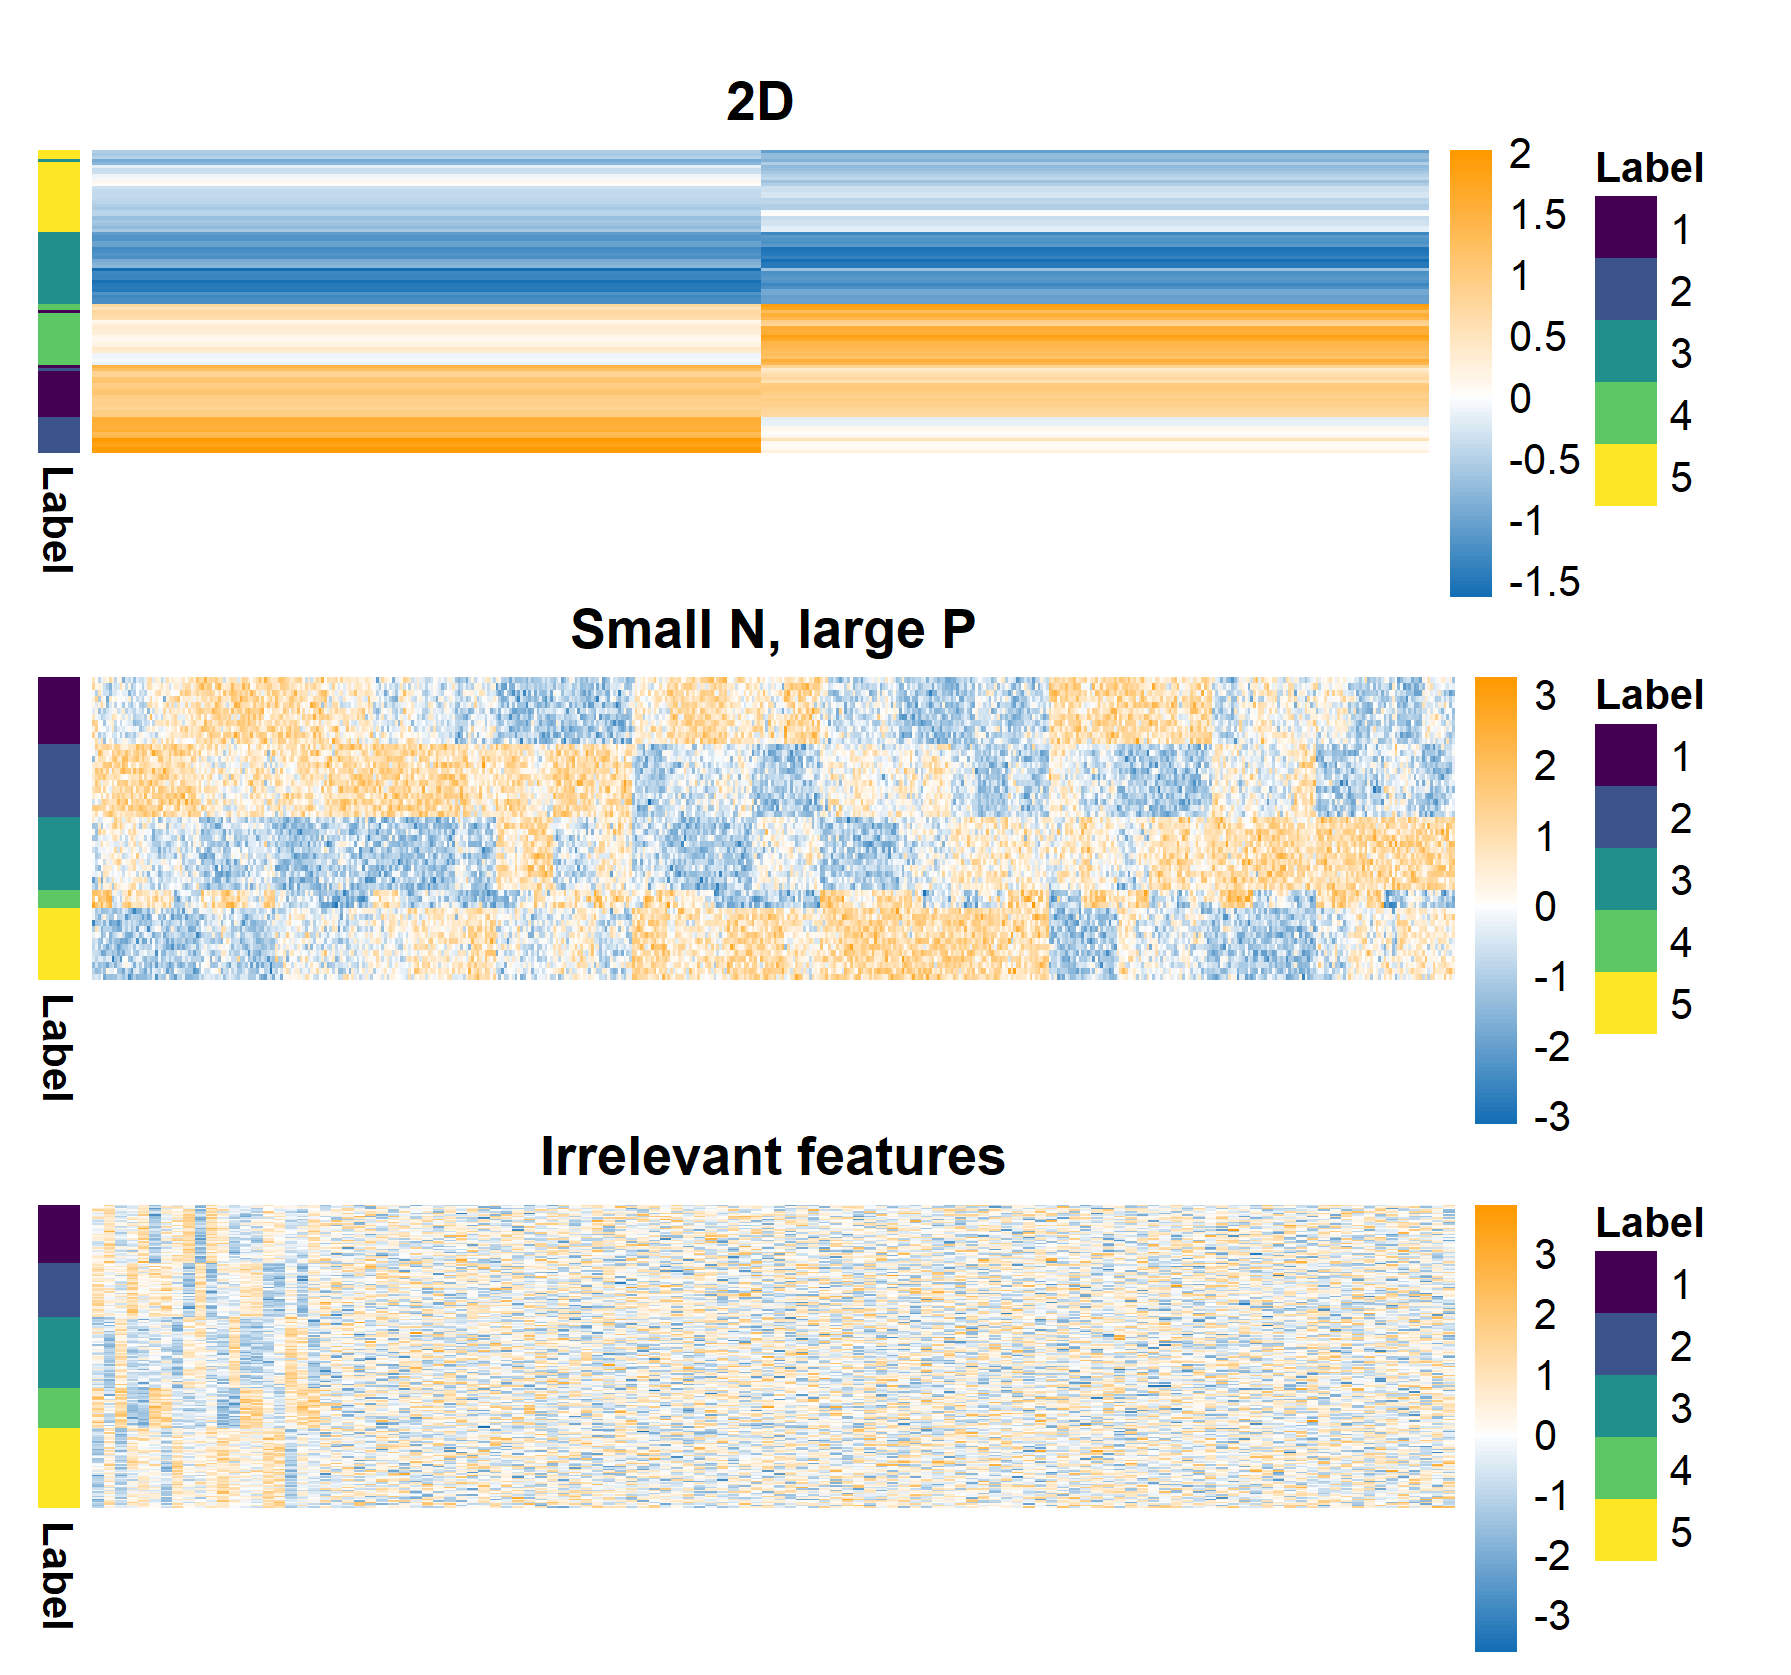
\includegraphics[scale=0.55]{./Images/Simulations/Data.png}
	\caption{Example of generated datasets. Each row is an item being clustered and each column a feature of generated data. The 2D dataset (which is ordered by hierarchical clustering here) should enable proper mixing of chains in the MCMC. The small $N$, large $P$ case has clear structure (observable by eye). This is intended to highlight the problems of poor mixing due to high dimensions even when the generating labels are quite identifiable. In the irrelevant features case, the structure is clear in the relevant features (on the left-hand side of this heatmap). This setting is intended to test how sensitive each approach is to noise.}
	\label{fig:genData}
\end{figure}

%\subsection{Data generating mechanism}
%We use the notation:
%
%\begin{itemize}
%	\item
%	\(N\): the number of items generated;
%	\item
%	\(P\): the number of features in the dataset;
%	\item
%	\(P_n\): the number of irrelevant features used;
%	\item
%	\(K\): the true number of clusters present;
%	\item
%	\(X = (x_1, \ldots, x_N)\): the items generated;
%	\item
%	\(\pi=(\pi_1, \ldots, \pi_K)\): the expected proportions of the population belonging to each cluster;
%	\item
%	\(c=(c_1, \ldots, c_N)\): the allocation variable for each item;
%	\item
%	\(\theta=(\theta_1, \ldots, \theta_K)\): the parameters associated with each component; and
%	\item
%	\(\phi=(\phi_1,\ldots, \phi_P)\): the indicator variable of feature relevance.
%\end{itemize}

%A description of the algorithm implementing this is given in algorithm \ref{algorithm:simulationGeneration}.

%\begin{figure}
%	\centering
%	\begin{tikzpicture}[background rectangle/.style={fill=white!1}, show background rectangle, scale=.4, auto,>=latex']
%		\tikzstyle{main}=[circle, minimum size = 10mm, thick, draw =black!80, node distance = 15mm]
%		\tikzstyle{connect}=[-latex, thick]
%		\tikzstyle{box}=[rectangle, draw=black!100]
%		%\node[main] (k) {$K$ };
%		\node[main, rectangle] (kappa) {$1$};
%		\node[main, rectangle] (xi) [left =of kappa] {$0$ };
%		\node[main, rectangle] (alpha) [left =of xi] {$1$ };
%%		\node[main] (k) [above =of alpha] {$K$};
%		\node[main, rectangle] (alpha2) [right =of kappa] {$2$ };
%		\node[main, rectangle] (beta) [right =of alpha2] {$2$ };
%		\node[main] (pi) [below =of alpha] {$\pi_k$ };
%		\node[main] (c_i) [below =of pi] {$c_i$};
%		\node[main] (mu) [below=of xi] {$\mu_{kp}$};		
%		\node[main] (sigma) [below =of alpha2] {$\sigma^2_{kp}$};
%		\node[main, fill = black!10] (x_i) [below =of mu] {$x_i$};
%     	\node[rectangle, inner sep=-0.5mm, fit= (c_i) (x_i),label=below right:$N$, xshift=13mm, yshift=-2mm] {};
%		\node[rectangle, inner sep=4.8mm,draw=black!100, fit= (c_i) (x_i)] {};
%		\node[rectangle, inner sep=-0.8mm, fit= (mu) (pi) (sigma),label=below right:$K$, xshift=43mm, yshift=-6mm] {};
%		\node[rectangle, inner sep=8.8mm, draw=black! 100, fit= (mu) (pi) (sigma)] {};
%		\node[rectangle, inner sep=-0.5mm, fit= (mu) (sigma),label=below right:$P$, xshift=26mm, yshift=-2mm] {};
%		\node[rectangle, inner sep=4.8mm, draw=black! 100, fit= (mu) (sigma)] {};
%		\path 
%%		(k) edge [connect, bend right=30] (pi)
%%		(k) edge [connect, bend left=30] (c_i)
%		%(k) edge [connect, bend left=30] (mu)
%		%(k) edge [connect] (sigma)
%		(alpha) edge [connect] (pi)
%		(pi) edge [connect] (c_i)
%		(alpha) edge [connect] (pi)
%		(c_i) edge [connect] (x_i)
%		(mu) edge [connect] (x_i)
%		(sigma) edge [connect] (x_i)
%		(xi) edge [connect] (mu)
%		(kappa) edge [connect] (mu)
%		(alpha2) edge [connect] (sigma)
%		(beta) edge [connect] (sigma)
%		%(k) edge[connect, bend right=30] (x_i)
%		;
%	\end{tikzpicture}
%	\caption{Directed acyclic graph for the Bayesian mixture of Gaussians used.}
%	\label{fig:simpleMixNormals}
%\end{figure}

%Data is generated using algorithm \ref{algorithm:simulationGeneration}.

%Within my generated datasets, there is a vector of means:
%
%\begin{align}
%\mu = (\mu_1, \ldots, \mu_K)
%\end{align}
%
%The indices here do not necessarily associate with the corresponding cluster (i.e.~\(\mu_1\) does not necessarily define the cluster labelled 1). Instead the mean vector is randomly permuted for each feature before generating the clusters; thus \(\nu\), the vector of means in the \(p^{th}\) feature, has the same values as \(\mu\) but reordered. It is the \(k^{th}\) value of \(\nu\) that defines the values generated for the \(k^{th}\) component in the \(p^{th}\) feature, not the \(k^{th}\) value from \(\mu\) (although \(\mu\) is one of the possible permutations of itself).
%
%As the mean of a cluster in a feature is sampled from \(\mu\), this means that additional features probably impart more information about the clustering structure.
%
%In my simulations there is a constant distance \(\Delta_{\mu}\) between each consecutive entry of \(\mu\), i.e.
%
%\begin{align}
%\mu = (\mu_1, \mu_1 + \Delta \mu, \ldots, \mu_1 + ( K - 1 ) \times \Delta \mu).
%\end{align}
%
%Thus \(\Delta \mu\) may be used as a defining parameter for the scenario rather than \(\mu\).


%\begin{algorithm} \label{algorithm:simulationGeneration}
%%	\KwData{\(X=(x_1, \ldots, x_N)\)}
%	\KwIn{
%%		A random seed $s$\\
%		Distance between means \(\Delta_{\mu}\)\\
%		A common standard deviation \(\sigma^2\)\\
%		A number of clusters \(K\)\\
%		The number of items to generate in total \(N\)\\
%		The number of features to generate in total \(P\)\\
%		An indicator vector of feature relevance \(\phi = (\phi_1, \ldots, \phi_P)\)\\
%		The expected proportion of items in each cluster \(\pi=(\pi_1, \ldots, \pi_K)\)\\
%		A method for sampling \(x\) times from the array \(y\), with weights \(\pi\): \emph{Sample}\((y, x)\)\\
%		A method for permuting a vector \(x\): \emph{Permute}\((x)\)\\
%		A method for generating a value from a univariate Gaussian distribution with mean \(\mu\) and standard deviation \(\sigma^2\): \emph{Gaussian}\((\mu, \sigma^2)\)\\
%	}
%	\KwOut{A dataset, $X$ \\ The generating cluster labels $c=(c_1, \ldots, c_N)$}
%	%	\KwResult{how to write algorithm with \LaTeX2e }
%	\Begin{
%%		\tcc{Set the random seed defining the sampling and permuting}
%%		$set.seed(s)$\;
%		\tcc{initialise the empty data matrix}
%		$X \leftarrow 0_{N \times P}$\;
%		\tcc{create a matrix of \(K\) means}
%		$\mu \leftarrow (\Delta_{\mu}, \ldots, K\Delta_{\mu})$\;
%		\tcc{generate the allocation vector}
%		\(c \leftarrow\) \emph{Sample}\((1:K, N, \pi)\)\;
%		
%		$\mathbf{M} \leftarrow \mathbf{0}_{N \times N}$\;
%		\For{$p = 1$ \KwTo $P$}{
%			\tcc{Test if the feature is relevant, if relevant generate data from a mixture of univariate Gaussians, otherwise draw all items from the same distribution}
%			\If{$\phi_p = 1$}{
%			
%%				\tcc{Permute the means associated with each cluster within the current feature to create independent features}
%				$\nu \leftarrow$ \emph{Permute}$(\mu)$\;
%	
%				\For{$n = 1$ \KwTo $N$}{
%%					\tcc{Generate data defined by the original label}
%					\(X(n, p) \leftarrow\) \emph{Gaussian}\((\nu_{c_n}, \sigma^2)\)
%				}
%			}
%		 \If{$\phi_p = 0$}{
%				\For{$n = 1$ \KwTo $N$}{
%					\(X(n, p) \leftarrow\) \emph{Gaussian}\((0, \sigma^2)\)
%				}
%			}
%		}
%		\tcc{Mean centre and scale the data}
%		$X \leftarrow Normalise(X)$
%	}
%	\caption{Data generation for a mixture of Gaussian with independent features. This algorithm is implemented in the \texttt{generateSimulationDataset} function from the \texttt{mdiHelpR} R package.}
%\end{algorithm}

%
%\hypertarget{study-design}{%
%	\subsection{Study design}\label{study-design}}
%
%\begin{sidewaysfigure}
%	\centering
%	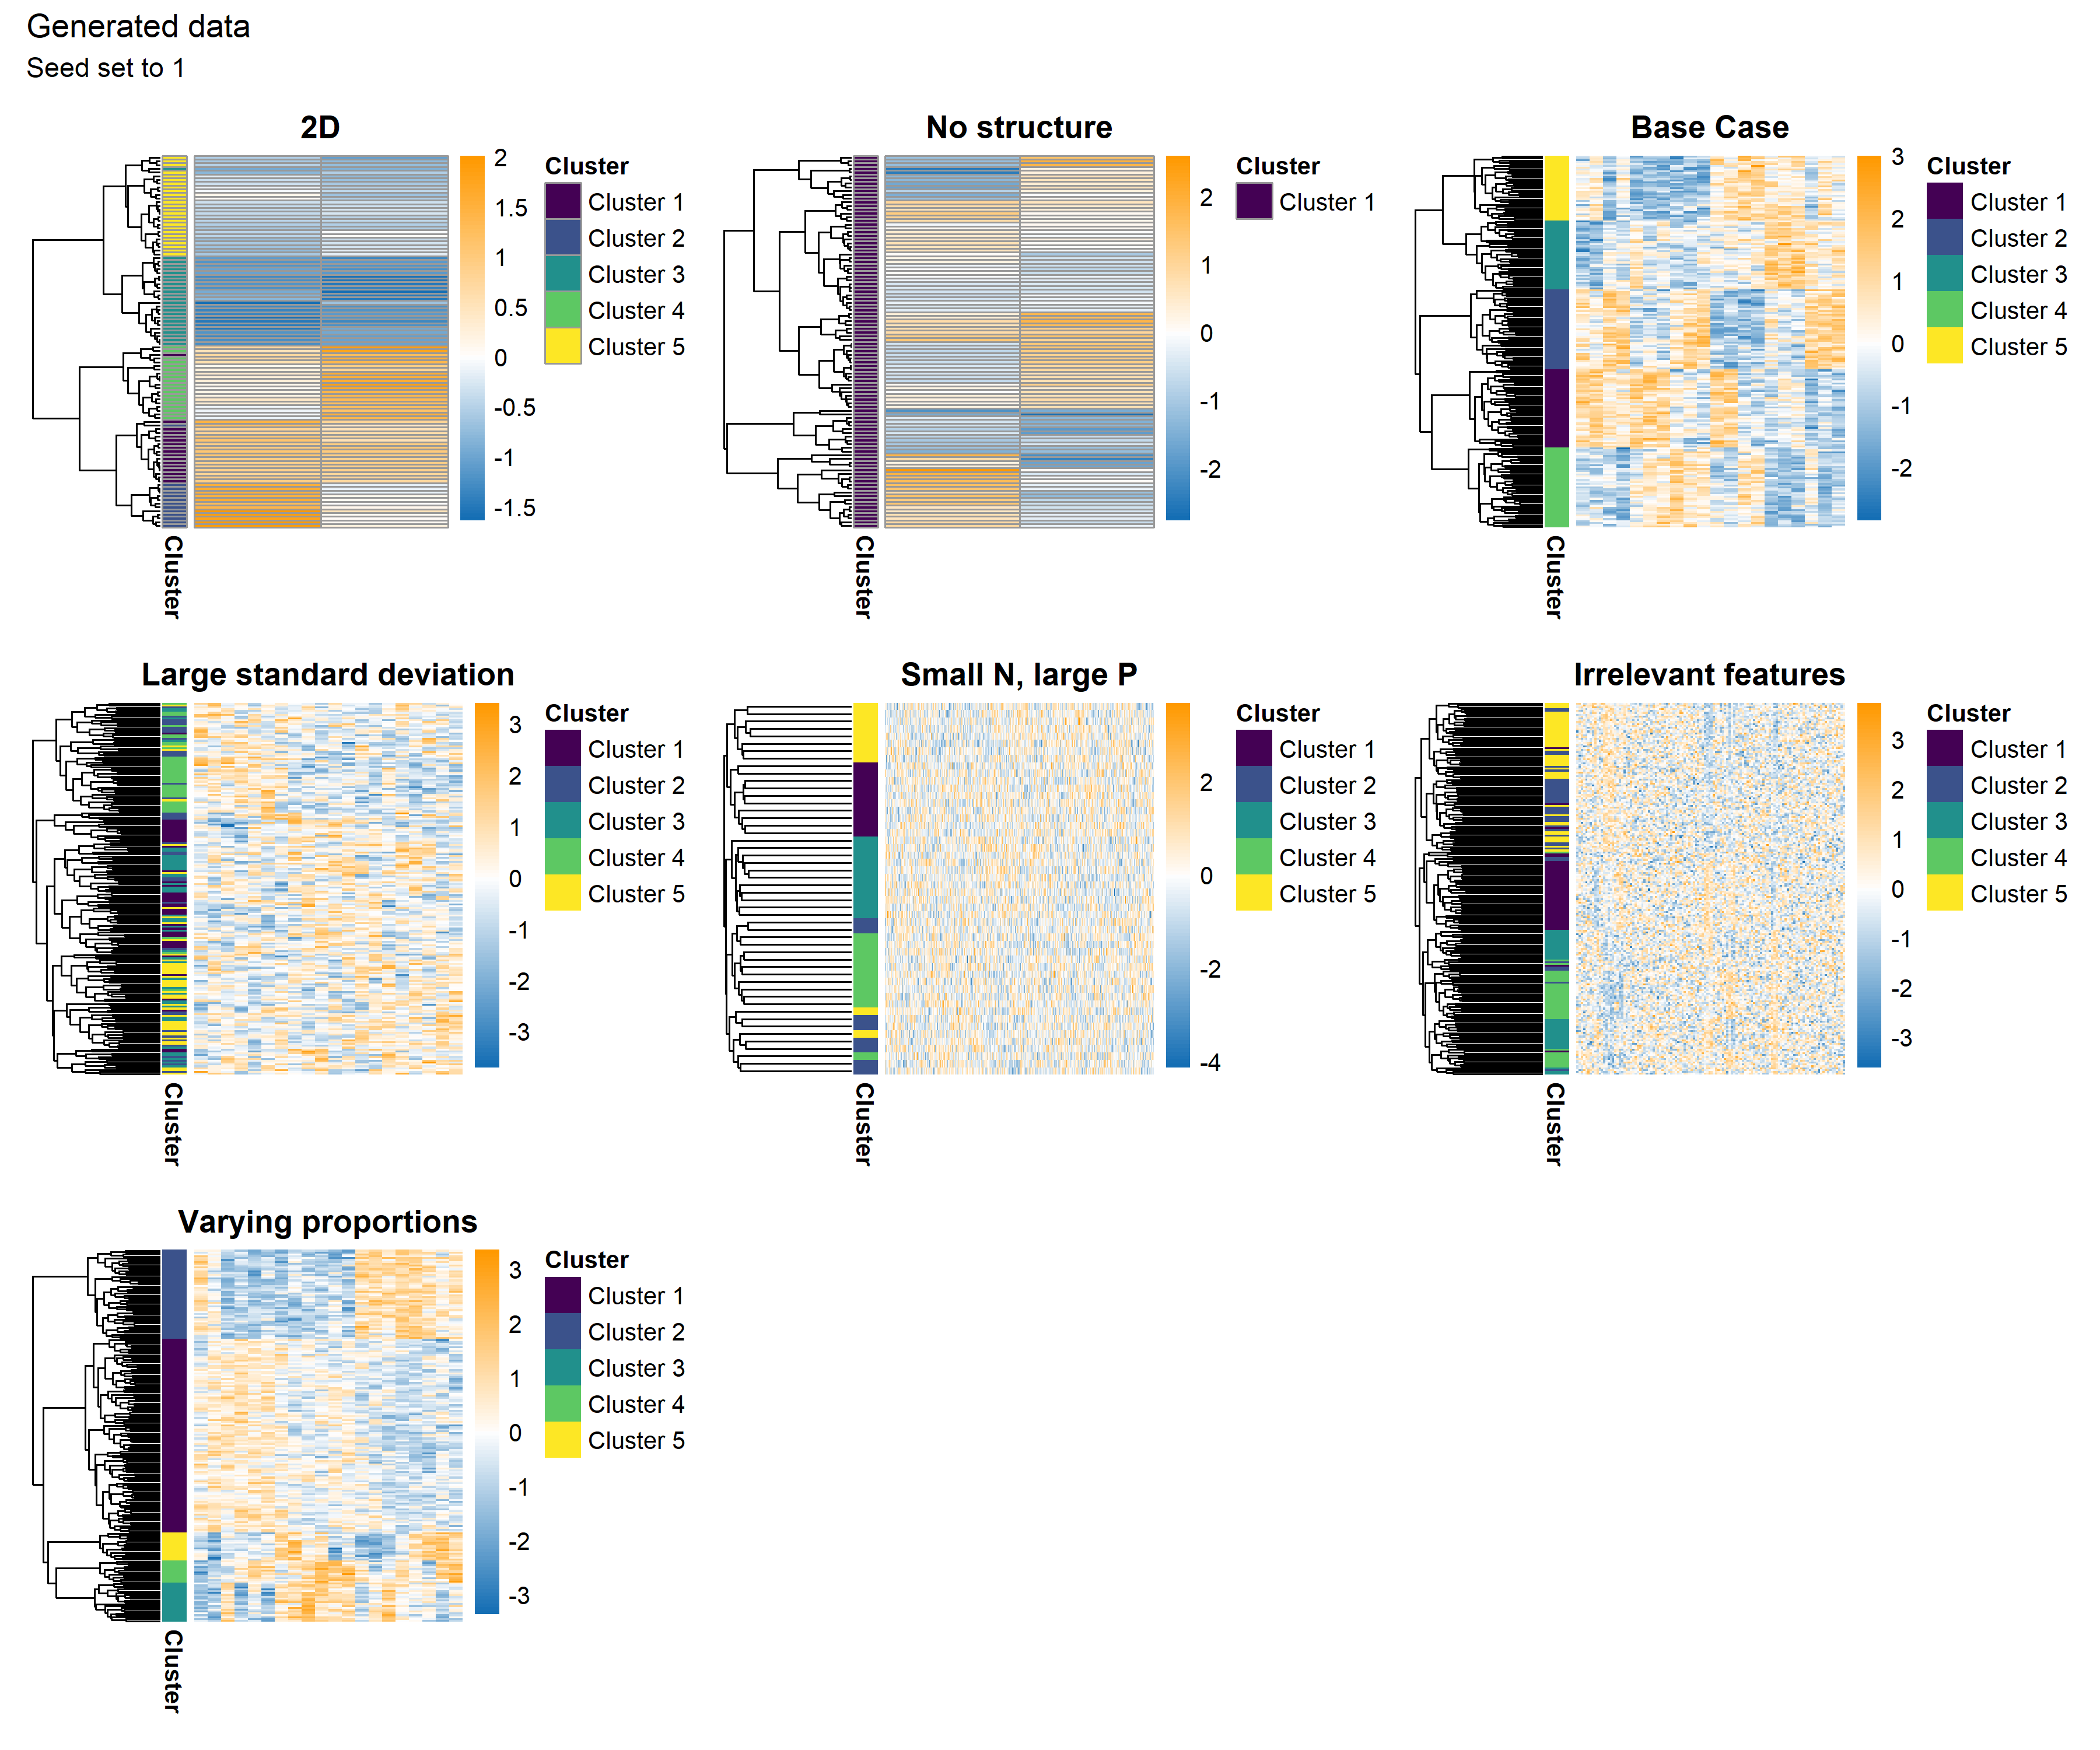
\includegraphics{./Images/Simulations/generated_datasets.png}
%	\caption{Example of generated datasets for different scenarios.}
%	\label{fig:genData}
%\end{sidewaysfigure}


%	\begin{sidewaysfigure}
%		\centering
%		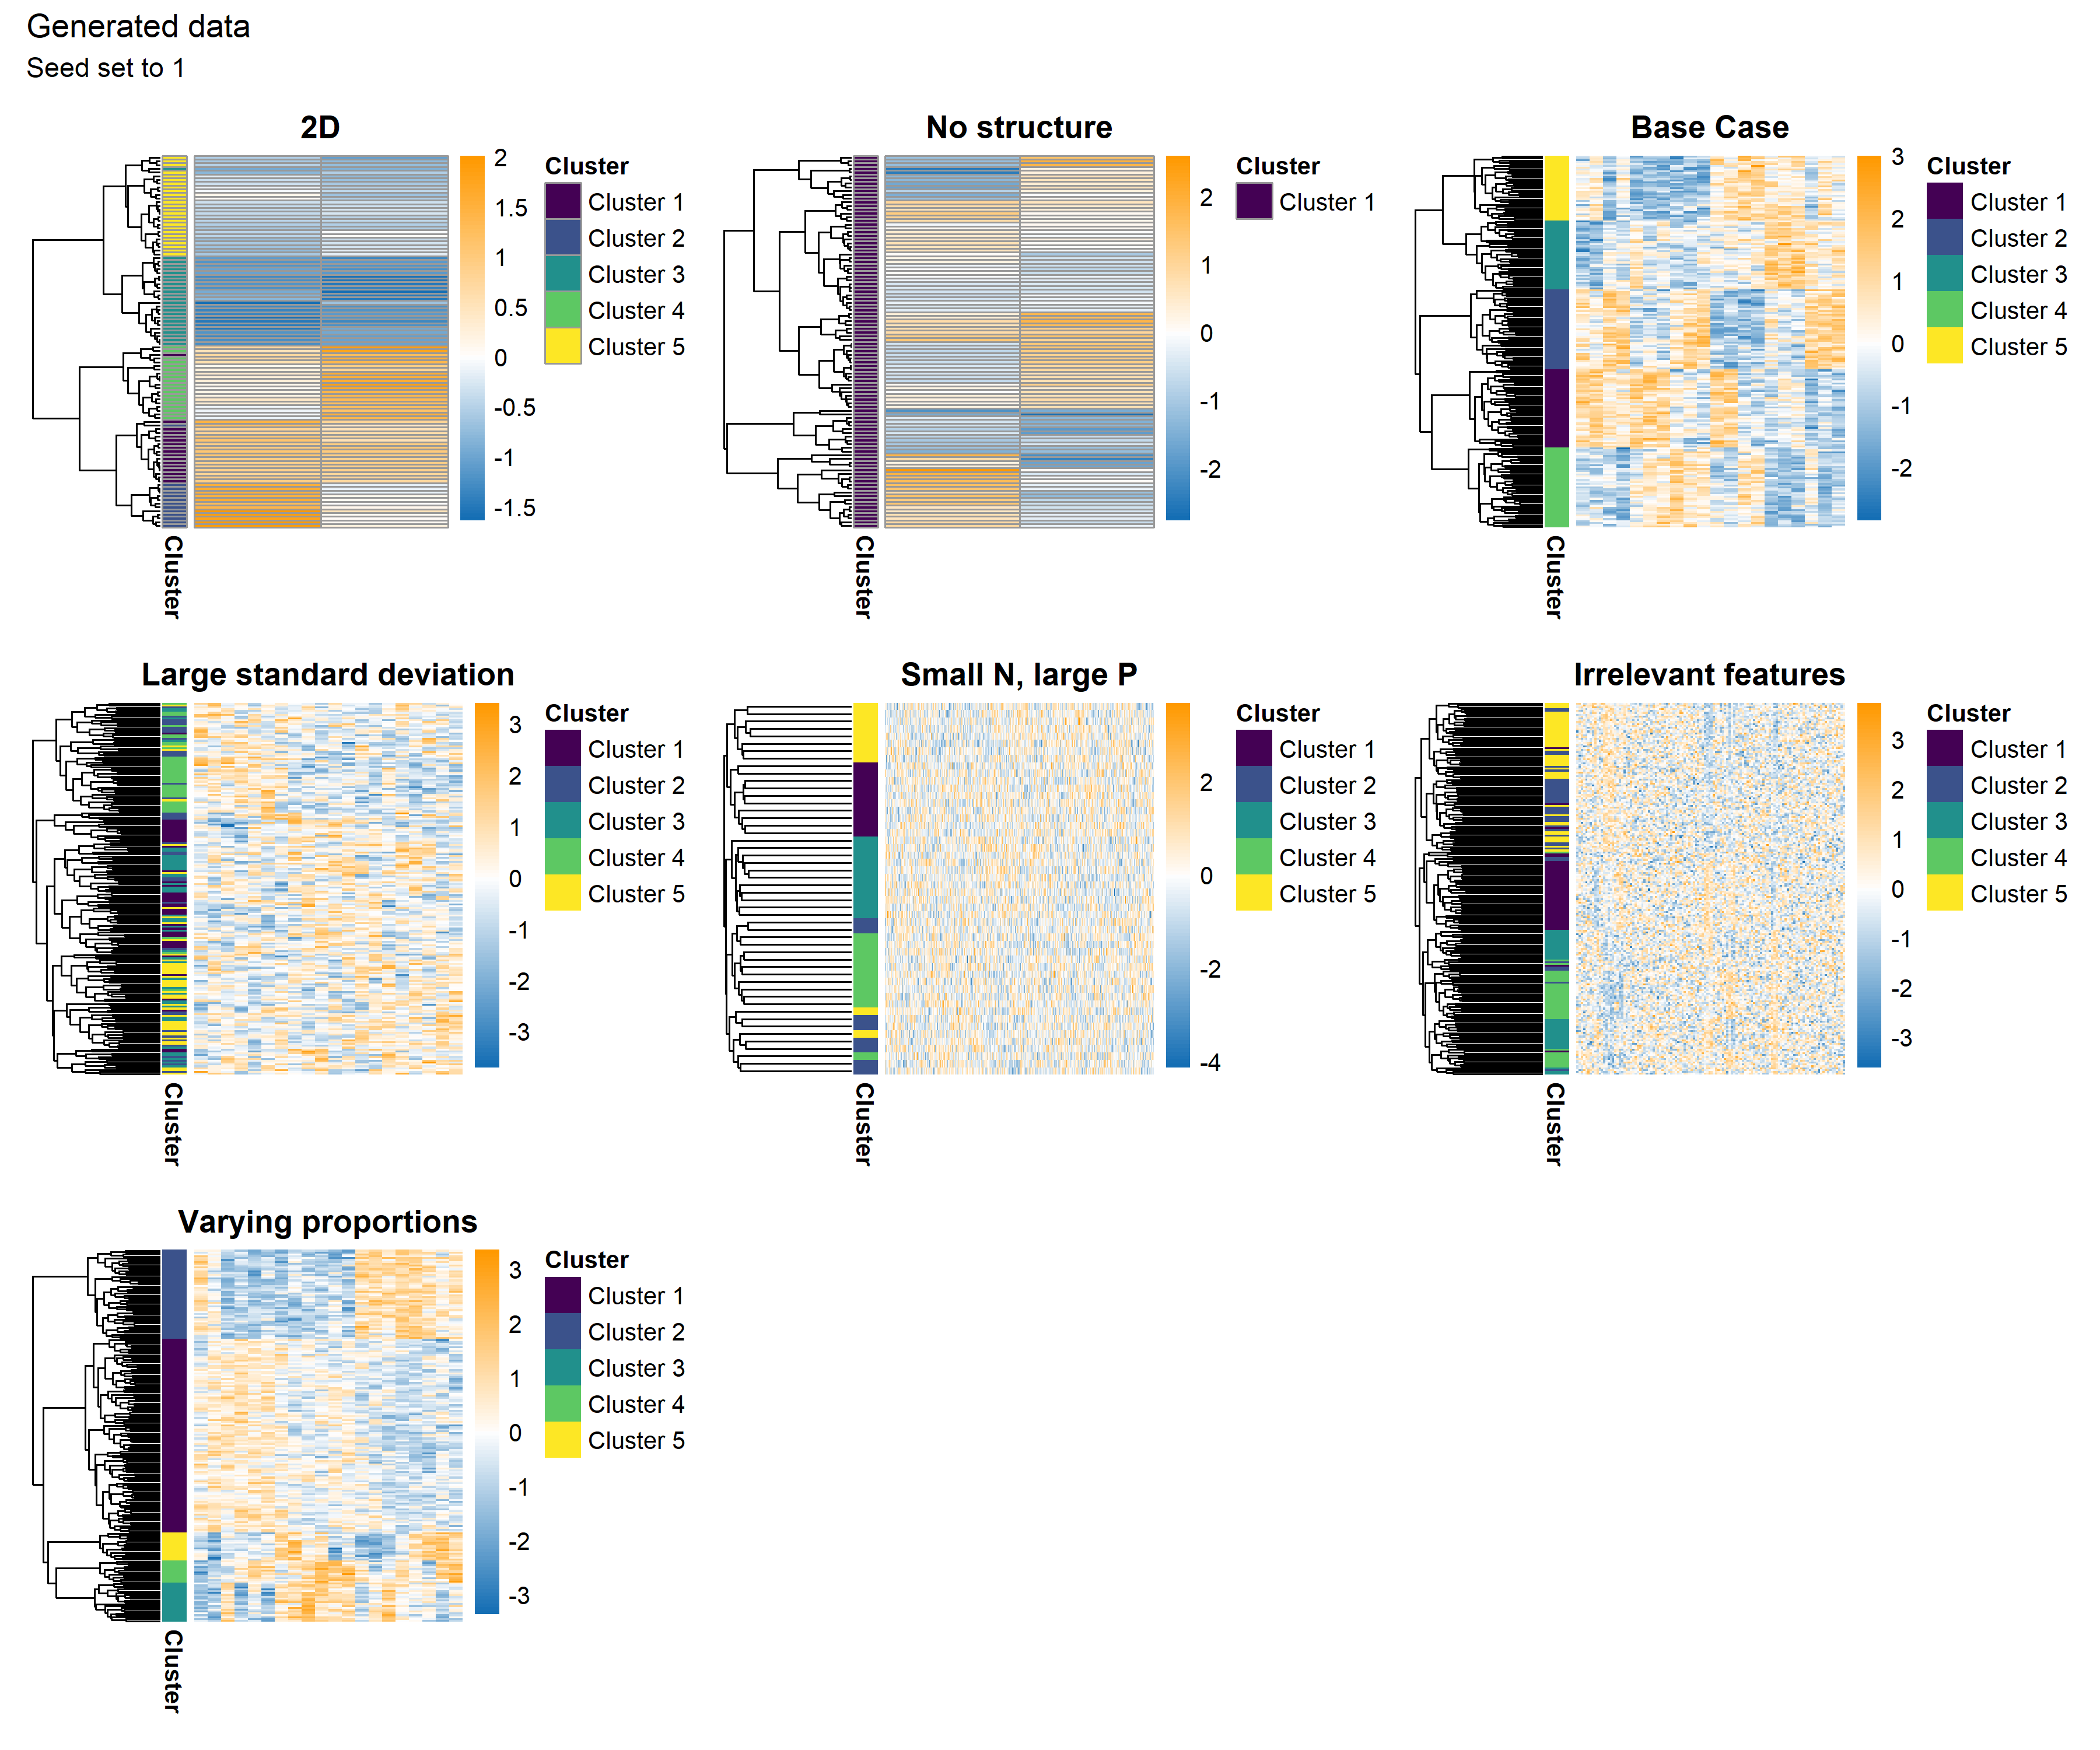
\includegraphics[scale=0.75]{./Images/Simulations/generated_datasets.png}
%		\caption{Example of generated datasets for different scenarios.}
%		\label{fig:genData}
%	\end{sidewaysfigure}


%\begin{tabular}{|l|ccccccc|}
%	\hline
%	\textbf{Scenario} & $N$ & $P_s$ & $P_n$ & $K$ & $\Delta_{\mu}$ & $\sigma^2$ & $\pi$\\
%	\hline 
%	Simple 2D & 100 & 2 & 0 & 5 & 3.0 & 1 &  $(\frac{1}{5} , \frac{1}{5}, \frac{1}{5}, \frac{1}{5}, \frac{1}{5})$ \\
%	%		\hline
%	No structure & 100 & 0 & 2 & 1 & 0.0 & 1 & 1 \\
%	%		\hline
%	Base Case & 200 & 20 & 0 & 5 & 1.0 & 1 &  $(\frac{1}{5} , \frac{1}{5}, \frac{1}{5}, \frac{1}{5}, \frac{1}{5})$\\
%	%		\hline
%	Large standard deviation & 200 & 20 & 0 & 5 & 1.0 & 3 & $(\frac{1}{5} , \frac{1}{5}, \frac{1}{5}, \frac{1}{5}, \frac{1}{5})$ \\
%	%		\hline
%	Large standard deviation & 200 & 20 & 0 & 5 & 1.0 & 5 &  $(\frac{1}{5} , \frac{1}{5}, \frac{1}{5}, \frac{1}{5}, \frac{1}{5})$\\
%	%		\hline
%	Irrelevant features & 200 & 20 & 10 & 5 & 1.0 & 1 &  $(\frac{1}{5} , \frac{1}{5}, \frac{1}{5}, \frac{1}{5}, \frac{1}{5})$\\
%	%		\hline
%	Irrelevant features & 200 & 20 & 20 & 5 & 1.0 & 1 &  $(\frac{1}{5} , \frac{1}{5}, \frac{1}{5}, \frac{1}{5}, \frac{1}{5})$\\
%	%		\hline
%	Irrelevant features & 200 & 20 & 100 & 5 & 1.0 & 1 &  $(\frac{1}{5} , \frac{1}{5}, \frac{1}{5}, \frac{1}{5}, \frac{1}{5})$\\
%	%		\hline
%	Varying proportions & 200 & 20 & 0 & 5 & 1.0 & 1 & $(\frac{1}{2} , \frac{1}{4}, \frac{1}{8}, \frac{1}{16}, \frac{1}{16})$ \\
%	Varying proportions & 200 & 20 & 0 & 5 & 0.4 & 1 &  $(\frac{1}{2} , \frac{1}{4}, \frac{1}{8}, \frac{1}{16}, \frac{1}{16})$ \\ %(0.5, 0.25, 0.125, 0.0675, 0.0675)\\
%	%		\hline
%	Small N, large P & 50 & 500 & 0 & 5 & 1.0 & 1 &  $(\frac{1}{5} , \frac{1}{5}, \frac{1}{5}, \frac{1}{5}, \frac{1}{5})$\\
%	%		\hline
%	Small N, large P & 50 & 500 & 0 & 5 & 0.2 & 1 &  $(\frac{1}{5} , \frac{1}{5}, \frac{1}{5}, \frac{1}{5}, \frac{1}{5})$
%%	\\
%%	\hline
%%	\caption{Parameters defining the simulation scenarios as used in generating data and labels.}
%	\label{table:scenarioTable}
%\end{tabular}

%Each scenario is seen as testing certain concepts or else specific characteristics of real data. An example of each scenario may be seen in Figure \ref{fig:genData}.


%The examples included are
%\begin{itemize}
%	\item a low-dimensional dataset,
%	\item a wide dataset representative of the \emph{small $N$, large $P$} paradigm prevalent in genetics, and
%	\item a dataset with a large number of irrelevant features.
%\end{itemize}
\noindent In each of these scenarios we apply a variety of methods (listd below) and compare the inferred point clusterings to the generating labels using the Adjusted Rand Index \citep[\textbf{ARI}][]{hubert1985comparing}.
\begin{itemize}
	\item \texttt{Mclust}, a maximum likelihood implementation of finite mixture models (for a range of modelled clusters, $K$),
	\item 10 chains of 1 million iterations, thinning to every thousandth sample for the overfitted Bayesian mixture model, and
	\item a variety of consensus clustering ensembles defined by inputs of $W$ chains and $D$ iterations within each chain (see algorithm \ref{algorithm:CCforBayesianMixtures}) with $W \in \{1, 10, 30, 50, 100\}$ and $D \in \{1, 10, 100, 1000, 10000\}$.
\end{itemize}
The ARI is a measure of similarity between two partitions,$c_1, c_2$, corrected for chance, with 0 indicating $c_1$ is no more similar to $c_2$ than a random partition would be expected to be and a value of 1 showing that $c_1$ and $c_2$ perfectly align. Details of how we used the methods in the simulation study can be found in sections 4.2, 4.3 and 4.4 of the Supplementary Material.

%For the 2D scenario \texttt{Mclust} and the individual long chains are expected to behave well, with no pathological behaviour emerging. In the other scenarios increasing dimensionality means that mixing problems can emerge and the chains become liable to being trapped in individual modes. 

%We compare consensus clustering of Bayesian mixture models to a traditional inference using several long chains of 1 million iterations (thinning to every thousandth) and \texttt{Mclust}. These are compared within a range of scenarios described in Table \ref{table:scenarioTable}. These test different settings represent of specific characteristics of datasets. We describe the results of three of these scenarios with the remainder described in the supplementary material.
%
%%We test different scenarios that change various parameters in this model. The scenarios tested and there defining parameters are shown in Table \ref{table:scenarioTable}. In this case the number of relevant features (\(P_s\)) is $\sum_p \phi_p$, and $P_n = P - P_s$.
%
%\begin{table}[ht]
%	\centering
%	\caption{Parameters defining the simulation scenarios as used in generating data and labels. Results for the \emph{Simple 2D}, the first \emph{Small N, large P} and final \emph{Irrelevant features} scenarios are shown in this report, please see the supplementary material for additional results. The number of relevant features (\(P_s\)) is $\sum_p \phi_p$, and $P_n = P - P_s$.}
%	\begin{tabular}{l|ccccccc}
%		\toprule
%		\textbf{Scenario} & $N$ & $P_s$ & $P_n$ & $K$ & $\Delta_{\mu}$ & $\sigma^2$ & $\pi$\\
%		\midrule
%		2D & 100 & 2 & 0 & 5 & 3.0 & 1 &  $(\frac{1}{5} , \frac{1}{5}, \frac{1}{5}, \frac{1}{5}, \frac{1}{5})$ \\
%		%		\hline
%%		No structure & 100 & 0 & 2 & 1 & 0.0 & 1 & 1 \\
%%		%		\hline
%%		Base Case & 200 & 20 & 0 & 5 & 1.0 & 1 &  $(\frac{1}{5} , \frac{1}{5}, \frac{1}{5}, \frac{1}{5}, \frac{1}{5})$\\
%%		%		\hline
%%		Standard deviation & 200 & 20 & 0 & 5 & 1.0 & 3 & $(\frac{1}{5} , \frac{1}{5}, \frac{1}{5}, \frac{1}{5}, \frac{1}{5})$ \\
%%		%		\hline
%%		Standard deviation & 200 & 20 & 0 & 5 & 1.0 & 5 &  $(\frac{1}{5} , \frac{1}{5}, \frac{1}{5}, \frac{1}{5}, \frac{1}{5})$\\
%%		%		\hline
%%		Irrelevant features & 200 & 20 & 10 & 5 & 1.0 & 1 &  $(\frac{1}{5} , \frac{1}{5}, \frac{1}{5}, \frac{1}{5}, \frac{1}{5})$\\
%%		%		\hline
%%		Irrelevant features & 200 & 20 & 20 & 5 & 1.0 & 1 &  $(\frac{1}{5} , \frac{1}{5}, \frac{1}{5}, \frac{1}{5}, \frac{1}{5})$\\
%%		%		\hline
%		Irrelevant features & 200 & 20 & 100 & 5 & 1.0 & 1 &  $(\frac{1}{5} , \frac{1}{5}, \frac{1}{5}, \frac{1}{5}, \frac{1}{5})$\\
%		%		\hline
%%		Varying proportions & 200 & 20 & 0 & 5 & 1.0 & 1 & $(\frac{1}{2} , \frac{1}{4}, \frac{1}{8}, \frac{1}{16}, \frac{1}{16})$ \\
%%		Varying proportions & 200 & 20 & 0 & 5 & 0.4 & 1 &  $(\frac{1}{2} , \frac{1}{4}, \frac{1}{8}, \frac{1}{16}, \frac{1}{16})$ \\ %(0.5, 0.25, 0.125, 0.0675, 0.0675)\\
%%		%		\hline
%		Small N, large P & 50 & 500 & 0 & 5 & 1.0 & 1 &  $(\frac{1}{5} , \frac{1}{5}, \frac{1}{5}, \frac{1}{5}, \frac{1}{5})$\\
%		%		\hline
%%		Small N, large P & 50 & 500 & 0 & 5 & 0.2 & 1 &  $(\frac{1}{5} , \frac{1}{5}, \frac{1}{5}, \frac{1}{5}, \frac{1}{5})$
%		%	\\
%		%	\hline
%%		\\
%		\botrule
%	\end{tabular}
%	\caption{Parameters defining the simulation scenarios as used in generating data and labels.}
%	\label{table:scenarioTable}
%\end{table}%
%
%The examples included are
%\begin{itemize}
%	\item a low-dimensional dataset,
%	\item a wide dataset representative of the \emph{small $N$, large $P$} paradigm prevalent in genetics, and
%	\item a dataset with a large number of irrelevant features.
%\end{itemize}
%The first of these is expected to be the setting where \texttt{Mclust} and the individual long chains behave well. In the other simulations increasing dimensionality means that mixing problems can emerge and the chains become liable to being trapped in individual modes. Within each simulation 100 datasets are generated.
% following algorithm \ref{algorithm:simulationGeneration}. 
%To each of these datasets, the following are applied

%\begin{itemize}
%	\item \texttt{mclust} (for a range of possible $K$),
%	\item 10 chains of 1 million iterations, thinning to every thousandth sample for the overfitted Bayesian mixture model, and
%	\item a variety of consensus clustering ensembles defined by inputs of $W$ chains and $D$ iterations within each chain (see algorithm \ref{algorithm:CCforBayesianMixtures}) with $W \in \{1, 10, 30, 50, 100\}$ and $D \in \{1, 10, 100, 1000, 10000\}$.
%\end{itemize}
%In theory we would expect the Bayesian chains to explore a common posterior distribution, but the practice sees chains become trapped in distinct modes in different scenarios. We believe that the mode within which the greatest number of chains become trapped would be that which is used to perform the inference in a real application (and longer chains did not solve the problem). As part of a pipeline where such analyses have to happen $12 \times 100 = 1,200$ times, we pool the Bayesian samples into a single Posterior Similarity Matrix (\textbf{PSM}) to aovid model selection problems. If the chains all explore the same space pooling the samples has little effect on the inference. Based upon visual inspection of the PSMs indicates that the disagreement between modes tends to be one of 
%\begin{itemize}
%	\item several clusters are merged or
%	\item a cluster is represented by two or more components,
%\end{itemize}
%each of the modes tends to have large overlap with all others. This means that the clustering inferred from the PSM created from the samples pooled across all stationary chains will represent the most popular mode and the metric of performance we use, the Adjusted Rand Index  will not be unduly inflated.
%The Frobenius norm between the PSM and the true coclustering will be less representative of a single chain as more modes will be represented and therefore greater uncertainty than any single chain. This is inline with our previous assertion that the Frobenius statistic is more an indicator that should be used along with visual assessment of examples of the PSMs and CMs from a simulation rather than sufficiently informative in and of itself.

\subsubsection{\texttt{Mclust}}
\texttt{Mclust} \citep{mclust2016scrucca} is a function from the R package \texttt{mclust}. It estimates and compares Gaussian mixture models based upon the maximum likelihood estimator of the parameters for a range of choices of $K$, the number of clusters used, and different covariance structures. The method initialises upon a hierarchical clustering of the data cut to $K$ clusters. The ``best'' model is determined using the Bayesian information criterion, \citep[][]{schwarz1978estimating}. See section 4.2 of the Supplementary Material for more details on how we applied \texttt{Mclust} to the simulated data.

\subsubsection{Bayesian inference}
%We use 10 long chains in where ``Bayesian inference'' is being considered in the simulations and the yeast analysis. In the simulations chains are kept in the analysis based upon a number of tests described below. To summarise the chains that are considered ``converged'' we pool the samples from across the chains (effectively using an ensemble of long chains). This choice is considered more in the supplementary materials. These pooled samples are expected to be an upper bound on the performance of any single chain in the simulations.


%I think have this in supplementary,remove from here.
%The model we use is a mixture of \emph{Gaussian} distributions.
% and thus \(\theta_{kp}=(\mu_{kp}, \sigma^2_{kp})\). The prior distributions used on the mixture parameters are
%\begin{align}
%	\pi_k \sim \textrm{Dirichlet}(\alpha, \ldots, \alpha), \hspace{0.5cm} \mu_{kp} \sim \mathcal{N}(\xi, \kappa), \hspace{0.5cm} \sigma_{kp}^2 \sim \Gamma^{-1}(a, b). \nonumber
%\end{align}
%The conditional independences and the priors used are shown in the directed acyclic graph (\textbf{DAG}) in Figure 1 in the supplementary materials.
%\ref{fig:simpleMixNormals}. 


%PROBLEM OF UNDEFINED DATASETS: We set the total number of occupied and empty components, $K_{max}$, to 50 in the simulations and 275 in the yeast analysis. 
% In practice where this $K$is unknown, $K_{max}$ is set to some large number.
% A component is a density in the mixture model; if a component is occupied than it forms a cluster and contributes to partitioning the sample.

To assess within-chain convergence of our Bayesian inference we use the Geweke $Z$-score statistic \citep{geweke1991evaluating}. Of the chains that appear to behave properly we then asses across-chain convergence using $\hat{R}$ \citep{gelman1992inference} and the recent extension provided by \cite{vats2018revisiting}. 

If a chain has reached its stationary distribution the Geweke $Z$-score statistic is expected to be normally distributed. Normality is tested for using a Shapiro-Wilks test \citep{shapiro1965analysis}. If a chain fails this test (i.e., the associated $p$-value is less than 0.05), we assume that it has not achieved stationarity and it is excluded from the remainder of the analysis.

The Vats and Knudson extension of $\hat{R}$ is a summary statistic for the entire chain; this is the primary indicator of failure for convergence, but a visualisation of the original $\hat{R}$ diagnostic is also considered. 

In theory we would expect the Bayesian chains to explore a common posterior distribution, but the practice sees chains become trapped in distinct modes in different scenarios. We believe that the mode within which the greatest number of chains become trapped would be that which is used to perform the inference in a real application (and longer chains did not solve the problem). As part of a pipeline where such analyses have to happen $12 \times 100 = 1,200$ times, we pool the Bayesian samples into a single Posterior Similarity Matrix (\textbf{PSM}, defined in section 1 of the Supplementary Material) to avoid model selection problems. If the chains all explore the same space pooling the samples has little effect on the inference. Based upon visual inspection of the PSMs indicates that the disagreement between modes in our simulations tends to be one of 
\begin{itemize}
	\item several clusters are merged or
	\item a generating cluster is represented by two or more components in the model,
\end{itemize}
each of the modes tends to have large overlap with all others. This means that the clustering inferred from the PSM created from the samples pooled across all stationary chains will represent the most popular mode and the metric of performance we use, the ARI will not be unduly inflated.

To infer a final clustering from the PSM, we use the \texttt{maxpear} function, as we do in the consensus clustering.

Details of the convergence diagnoses and \texttt{maxpear} in a Bayesian setting are given in section 4.3 of the Supplementary Material.

%We use the \texttt{maxpear} function \citep{fritsch2009improved} from the R package \texttt{mcclust} \citep{fritsch2012mcclust} to infer a point clustering from the PSM of a long chain (some details of which are given in section 4.2 of the Supplementary Material). %Consensus matrices.

%A deeper consideration of the convergence of chains is included in the Supplementary Materials.

%\subsection{Simulated data methods}
%\subsubsection{Mixture models}
%We write the basic mixture model for independent items $X=(x_1, \ldots, x_N)$ as 
%\begin{align}
%	x_n \sim \sum_{k=1}^K\pi_k f(x_n | \theta_k) \hspace{1cm} \textrm{independently for $n = 1,\ldots,N$}
%\end{align}
%where $f(\cdot| \theta)$ is some family of densities parametrised by $\theta$, with each $f(\cdot| \theta)$ being a \emph{component} of the mixture model. A common choice is the Gaussian density function, with $\theta=(\mu, \sigma^2)$. $K$, the number of components modelled, $\{\theta_k\}_{k=1}^K$, the component parameters, and $\pi=(\pi_1, \ldots, \pi_K)$, the component weights are the objects to be inferred. In clustering, such a model arises due to the belief that the population from which the random sample under analysis has been drawn consists of $K$ unknown groups proportional to $\pi$, with each component describing one of these subpopulations. In this setting it is natural to include a latent \emph{allocation variable}, $c=(c_1, \ldots, c_N)$, to indicate which group each item is drawn from. As the number of sub-groups present in the sample may be less than that of the population, some components may have no allocated items. In this case each non-empty component of the mixture corresponds to a cluster. The model is
%\begin{equation}
%	\label{eqn:mixModel}
%	\begin{array}{r@{}l l}
%		p(c_n = k) = \pi_k&  &\textrm{for $k = 1,\ldots,K$,} \\
%		x_n | c_n \sim f(x_n | \theta_k)& &\textrm{independently for $n = 1,\ldots,N$.} 
%	\end{array}
%\end{equation}
%More details of the mixture model can be found in section 2.1 of the Supplementary Material.

\subsection{Analysis of the cell cycle in budding yeast}
\subsubsection{Datasets}
We aim to create clusters of genes that are co-expressed, have common regulatory proteins and share a biological function. To achieve this, we use three datasets that were generated using different 'omics technologies and target different aspects of the molecular biology underpinning the cell cycle process.
\begin{itemize}
	\item Microarray profiles of RNA expression from \cite{granovskaia2010high}. This dataset comprises measurements of cell-cycle-regulated expression at 5-minute intervals for 200 minutes (up to three cell division cycles) and is referred to as the \textbf{time course} dataset. The cells are synchronised at the START checkpoint in late G1-phase using alpha factor arrest
	%, with the number of budding cells monitored to asses the degree of synchrony 
	\citep{granovskaia2010high}. We include only the genes identified by \cite{granovskaia2010high} as having periodic expression profiles.
%	 This includes some non-coding RNAs (\textbf{ncRNAs}) of which the majority are anti-sense RNAs.
	\item Chromatin immunoprecipitation followed by microarray hybridization (\textbf{ChIP-chip}) data from \cite{harbison2004transcriptional}. This dataset discretizes $p$-values from tests of association between 117 DNA-binding transcriptional regulators and a set of yeast genes. Based upon a significance threshold these $p$-values are represented as either a 0 (no interaction) or a 1 (an interaction).
	\item Protein-protein interaction (\textbf{PPI}) data from BioGrid \citep{stark2006biogrid}. This database consists of of physical and genetic interactions between gene and gene products. The interactions included are a collection of results observed in high throughput experiments and some computationally inferred interactions. The dataset we used contained 603 proteins as columns. An entry of 1 in the $(i, j)^{th}$ cell indicates that the $i^{th}$ gene has a protein product that is believed to interact with the $j^{th}$ protein.
\end{itemize}
%We believe such informed gene sets are more relevant to phenotypic traits and offer insight into more complex biological processes. 
%We believe that the integrative aspect of the analysis means that the clusters are more interpretable than in a standalone cluster analysis. Cluster analysis of a single dataset entails interpreting the clusters defined by similarity within a single experiment which often involves strong assumptions about the biological processes behind the result (e.g., correlation of transcripts implies co-regulation).
The datasets were reduced to 551 items by considering only the genes with no missing data in the PPI and ChIP-chip data. The choices to reduce the datasets to these 551 genes are the same steps as in \cite{kirk2012bayesian}. 

\subsubsection{Multiple dataset integration}
We applied consensus clustering to MDI for our integrative analysis. MDI jointly models the clustering in each dataset, inferring individual clusterings for each dataset that are informed by similarity in the other clusterings. MDI learns the similarity between the datasets being analysed and does not assume global structure. This means that the similarity between datasets is not strongly assumed in our model; individual clusters or genes that align across datasets are based solely upon the evidence present in the data not strong modelling assumptions. Thus, datasets that share less common information can be included without fearing that this will warp the final clusterings in some way.
% we can include the PPI data and expect it to contribute to our final clustering despite the expectation that there will be less shared information between the time course  dataset with its large set of ncRNAs might and this PPI dataset. 
For more details on MDI see section 2.2 of the Supplementary Material and \cite{kirk2012bayesian}.

%The datasets are shown in Figure \ref{fig:yeastData}.
The datasets were modelled using a mixture of Gaussian processes in the time course dataset and Multinomial distributions in the ChIP-chip and PPI datasets. 
%To ensure that our mixture model is initially overfitted we set $K_{max}=275\approx\frac{N}{2}$.

%the 551 yeast genes considered in the original MDI paper \citep{kirk2012bayesian} in an integrative setting. This consists of three datasets
%\begin{itemize}
%	\item  ChIP data from \cite{harbison2004transcriptional},
%	\item binary PPI data obtained from BioGRID \citep{stark2006biogrid} and 
%	\item a gene expression time course dataset from \cite{granovskaia2010high}.
%\end{itemize}
%The clustering in these datasets is modelled using MDI. We use 10 chains of 676,000 iterations (the number of iterations performed in 36 hours on the slowest chain) and consensus clustering of 100 chains of 500 iterations. The ChIP and PPI data are modelled using mixtures of multinomial distributions and the time course data by a mixture of Gaussian processes \citep[with dataset density choice following the original paper by ][]{kirk2012bayesian}.


%Multiple dataset
%\begin{itemize}
%	\item MDI yeast
%	\item BCC?
%	\item PanCancer data\vspace*{1pt}
%\end{itemize}


\section{Results}
\subsection{Simulated data}
%The methods used are 
%\begin{itemize}
%	\item \texttt{Mclust} (for a range of possible $K$),
%	\item 10 chains of 1 million iterations, thinning to every thousandth sample for the overfitted Bayesian mixture model, and
%	\item a variety of consensus clustering ensembles defined by inputs of $W$ chains and $D$ iterations within each chain with $W \in \{1, 10, 30, 50, 100\}$ and $D \in \{1, 10, 100, 1000, 10000\}$.
%\end{itemize}
We use the ARI between the generating labels and the inferred clustering of each method to be our metric of predictive performance.
\begin{figure} %[!tpb]
	\centering
	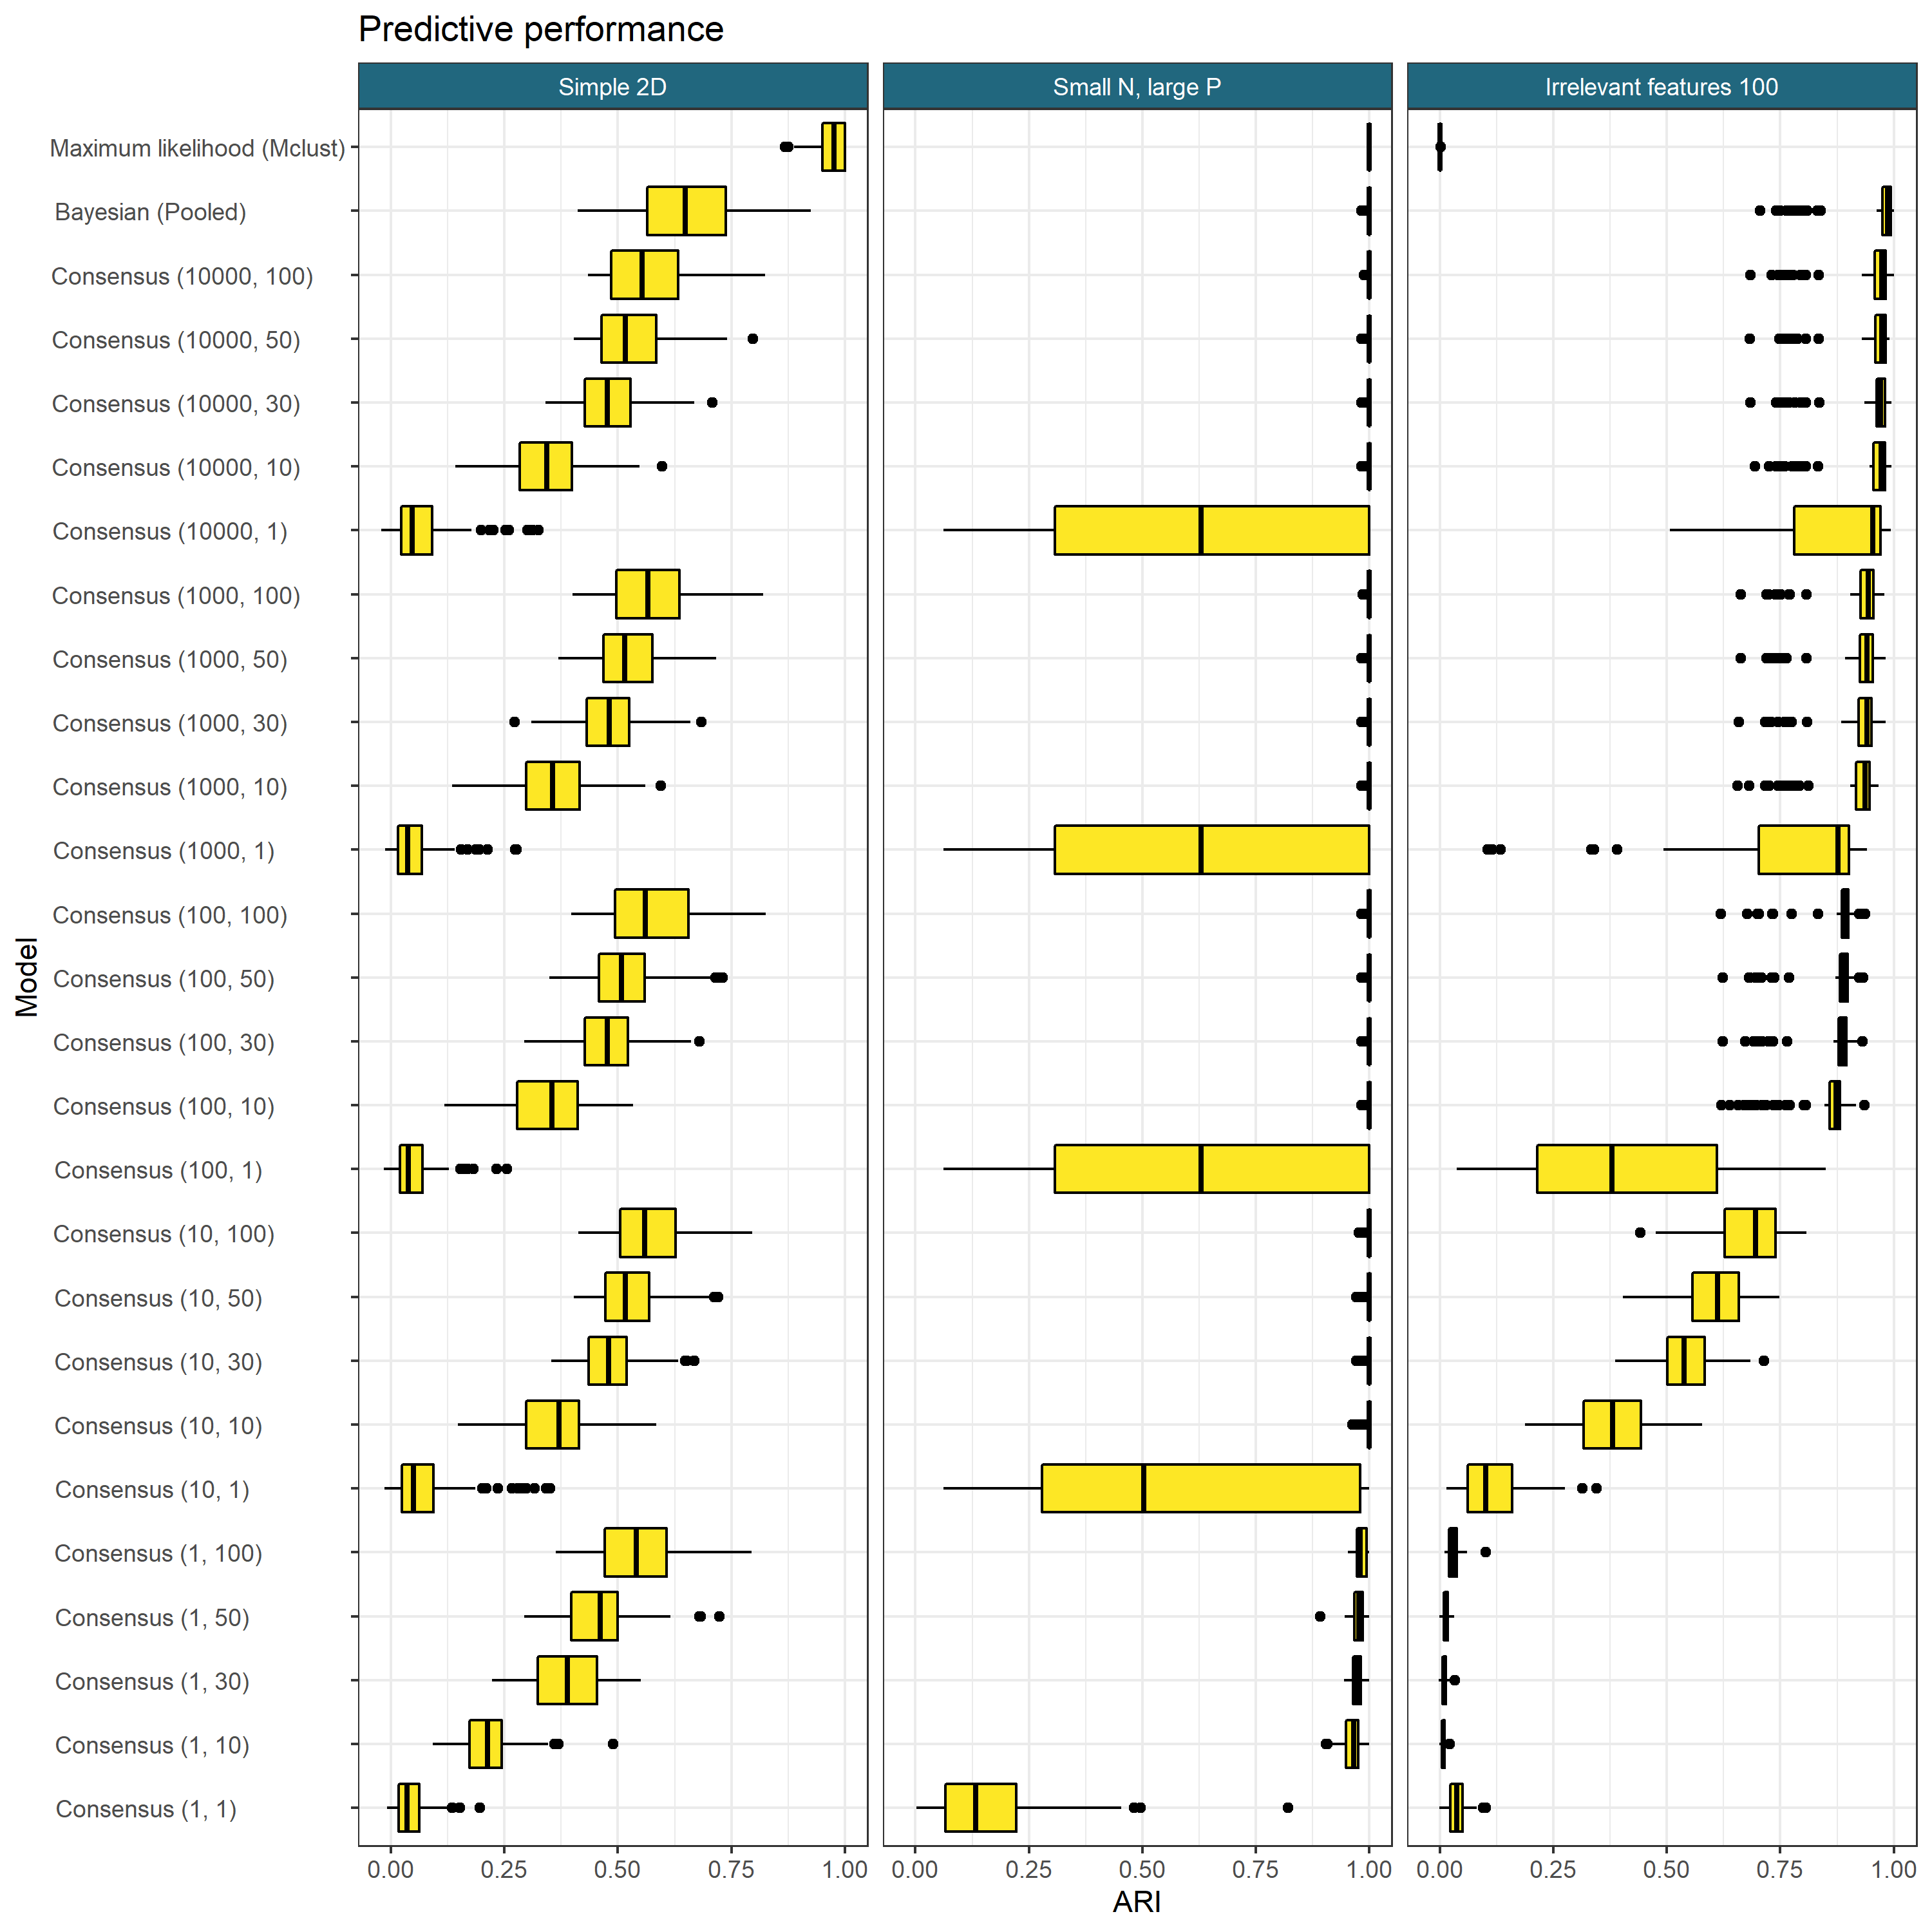
\includegraphics[scale=0.55]{./Images/Simulations/simulation_model_prediction.png}
	\caption{Model performance in the 100 simulated datasets for each scenario, defined as the ARI between the generating labels and the inferred clustering. $CC(d, w)$ denotes consensus clustering using the clustering from the $d^{th}$ iteration from $w$ different chains. }
	\label{fig:simResults}
\end{figure}
A summary of the results for a selection of the simulation scenarios are shown in 
%Table \ref{table:meanARISims} and 
Figure \ref{fig:simResults}. In the 2D and Small $N$, large $P$ scenarios, \texttt{Mclust} performs very well, correctly identifying the true structure However, a large number of irrelevant features completely erodes the ability of \texttt{Mclust} to uncover subpopulation structure. Instead, the method is blinded by the irrelevant features and identifies a clustering of $K=1$. 

The pooled samples from multiple long chains performs very well. This suggests that the pooling effect means that any multi-modality present in the data is less of a problem. In this case the pooled samples, themselves a consensus of 10 models, acts as an upper bound on the more practical implementations of consensus clustering and any individual long chain. 

Consensus clustering does uncover some of the generating structure in the data, even using a small number of short chains. With sufficiently large ensembles and chain depth, consensus clustering is close to the pooled Bayesian samples in predictive performance.

For the consensus clustering methods, we can also see from Figure \ref{fig:simResults}, that for a constant chain depth increasing the number of chains used follows a pattern of diminishing returns. There are strong initial gains for a greater ensemble width, but the improvement decreases for each successive chain. A similar pattern emerges in increasing chain length for a constant number of chains. 
%This fits the pattern we expected in making our stopping rule for ensemble growth in section \ref{sec:ensembleChoice}. We also notice that the consensus clustering appears bound by some asymptote, apparently defined by the pooled long chains.

If we look beyond the ARI at the PSMs and consensus matrix for one of the ensembles in Figure \ref{fig:simSmallNLargePPSMs}, we see very little difference between the similarity matrix from the pooled samples and the consensus clustering. Similar clusters emerge, and we see comparable confidence in the pairwise clusterings. In the next two rows the PSMs constructed from 6 of the long chains that passed the stationarity test are displayed. Each PSM is binary, with all entries being 0 or 1. This means only a single clustering is sampled within each chain, implying very little uncertainty in the partition. However, three different modes emerge across the chains showing that the chains are failing to explore the full support of the posterior distribution of the clustering. This shows that consensus clustering is exploring more possible clusterings than any individual chain and explores a similar space to the union of the samples from the long chains.

% In terms of the Frobenius norm, many of the consensus clustering results have significant overlap with the pooled long chains.

%\begin{table}[!htbp] \centering 
%	\caption{Median ARI for 100 datasets within three simulation scenarios between the generating labels and the predicted clustering for a subset of methods. CC($d, w$) indicates consensus clustering using the $d^{th}$ sample from $w$ chains. As in Figure \ref{fig:simResults}, the diminishing returns for increasing chain length or chain depth can be seen.} 
%	\begin{tabular}{@{\extracolsep{1pt}} l|ccc} 		
%		\hline \\[-1.8ex] 
%		\textbf{Method} & 2D & Small N, large P & Irrelevant features \\ 
%		\hline \\[-1.8ex] 
%		\hline \\[-1.8ex] 
%		Mclust & $0.976$ & $1.000$ & $0.000$ \\ 
%		Bayesian (Pooled) & $0.648$ & $1.000$ & $0.986$ \\ 
%		CC(10000, 100) & $0.553$ & $1.000$ & $0.974$ \\
%		CC(10000, 50) & $0.516$ & $1.000$ & $0.974$ \\ 
%		CC(10000, 10) & $0.343$ & $1.000$ & $0.971$ \\ 
%		CC(100, 100) & $0.561$ & $1.000$ & $0.892$ \\ 
%		CC(100, 50) & $0.508$ & $1.000$ & $0.889$ \\ 
%		CC(100, 10) & $0.355$ & $1.000$ & $0.872$ \\ 
%		CC(10, 100) & $0.559$ & $1.000$ & $0.695$ \\ 
%		CC(10, 50) & $0.516$ & $1.000$ & $0.611$ \\ 
%		CC(10, 10) & $0.370$ & $1.000$ & $0.380$ \\ 		
%		\hline  %\\[-1.8ex] 
%	\end{tabular} 
%\label{table:meanARISims} 
%\end{table} 

%\begin{table}[ht]
%	\centering
%	\caption{Mean ARI for 100 datasets within three simulation scenarios between the generating labels and the predicted clustering for a subset of methods. CC($r, s$) indicates consensus clustering using the $r^{th}$ sample from $s$ chains.}
%	\begin{tabular}{l|ccc}
%		\toprule
%		\textbf{Model} & 2D & Small $N$, large $P$ & Irrelevant features \\
%		\midrule
%		Mclust & 0.970 &       1.000 &         0.000\\
%		Bayesian (Pooled) &  0.669 & 				0.999 &         0.946\\
%		CC(10, 10) & 0.362 &	            0.997 &         0.385\\
%		CC(100, 10) & 0.844 &			    0.346 &         0.999\\
%		CC(100, 50) & 0.873 &			    0.517 &         0.999\\
%		CC(100, 100) & 0.879 &  			0.576 &         0.999\\
%		CC(10000, 10) & 0.348 &             0.999 &			0.935\\
%		CC(10000, 100) & 0.570 &            0.999 &			0.944\\
%		\botrule
%	\end{tabular}
%%	\label{table:meanARISims}
%\end{table}
%It can be seen from table \ref{table:meanARISims} and Figure \ref{fig:simResults} that 

\begin{figure} %[!tpb]
	\centering
	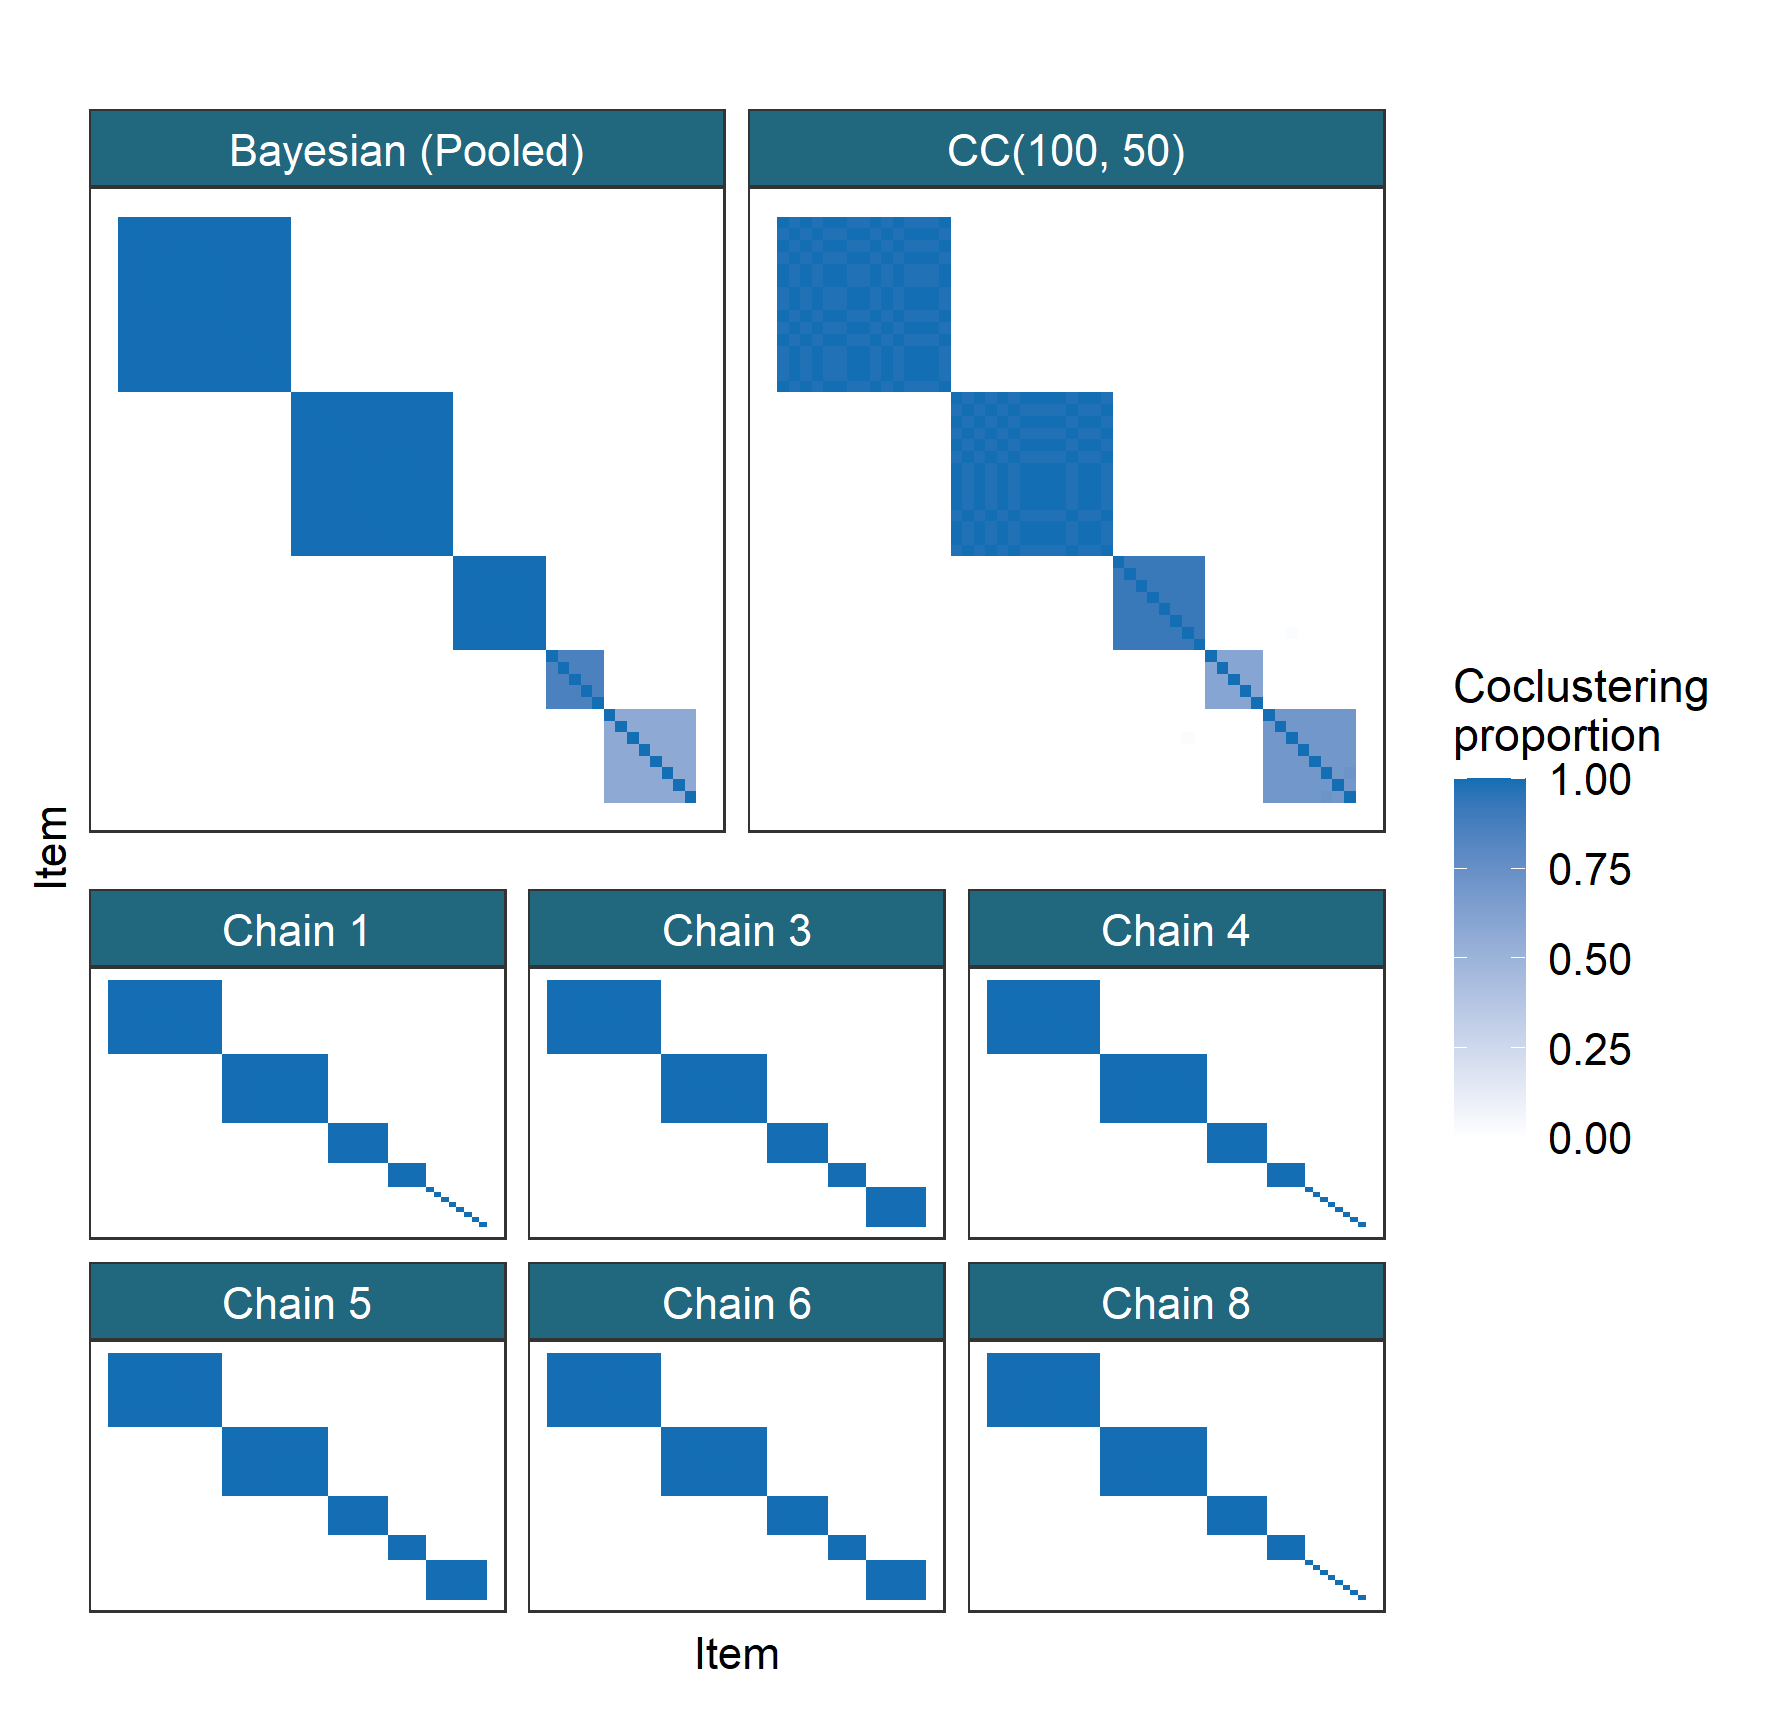
\includegraphics[scale=0.17]{./Images/Simulations/small_n_large_p_base/comp_psms_cm_edited.png}	
%PSMs/BayesianSimulation2PSMs.png}
%	\caption{PSMs for 8 chains that pass within chain convergence test. Rows and columns are ordered by a hierarchical clustering applied to the matrix in the bottom right. Annotations are the generating labels. The top row of PSMs are all in a common mode where Cluster 3 does not merge instead remaining as singletons. In the bottom row the first, second and fourth matrices correctly cluster all 5 clusters. The third matrix uncovers a different mode where Cluster 5 does not merge. The matrices appear binary, suggesting no diversity in the partitions being sampled.}
	\caption{Comparison of similarity matrices from a dataset for the Small $N$, large $P$ scenario. In each matrix, the $(i, j)^{th}$ entry is the proportion of clusterings for which the $i^{th}$ and $j^{th}$ items co-clustered for the method in question. In the first row the PSM of the pooled Bayesian samples is compared to the CM for CC(100, 50), with a common ordering of rows and columns in both heatmaps. In the following rows, 6 of the long chains that passed the tests of convergence are shown.}
	\label{fig:simSmallNLargePPSMs}
\end{figure}

Figure \ref{fig:simSmallNLargePPSMs} shows an example of different long chains becoming trapped in different modes and failing to explore a common partition space. We see that if any one chain is used then some of the uncertainty that should be present, some part of the target distribution, is discarded as each chain only represents a single possible clustering. Interestingly, if we take the union of the long chains and construct a similarity matrix, which might be considered to have sampled from various parts of the posterior distribution, this is more similar to the consensus matrix for a number of short chains than it is to any single long chain (as seen in the similarity of the PSM for the Bayesian (Pooled) and CC(100, 50) in Figure \ref{fig:simSmallNLargePPSMs}), suggesting that the consensus matrix is describing the uncertainty present in the final clustering more fully than any single long chain.
%In the simulations shown here the overlap between the modes and signal in the data is clear enough that one can pick the true clustering structure and select the chain that best represents this, but in a real analysis additional steps would have to be followed to decide upon which chain best represented the posterior distribution before proceeding in the analysis.

\begin{figure} %[!tpb]
	\centering
	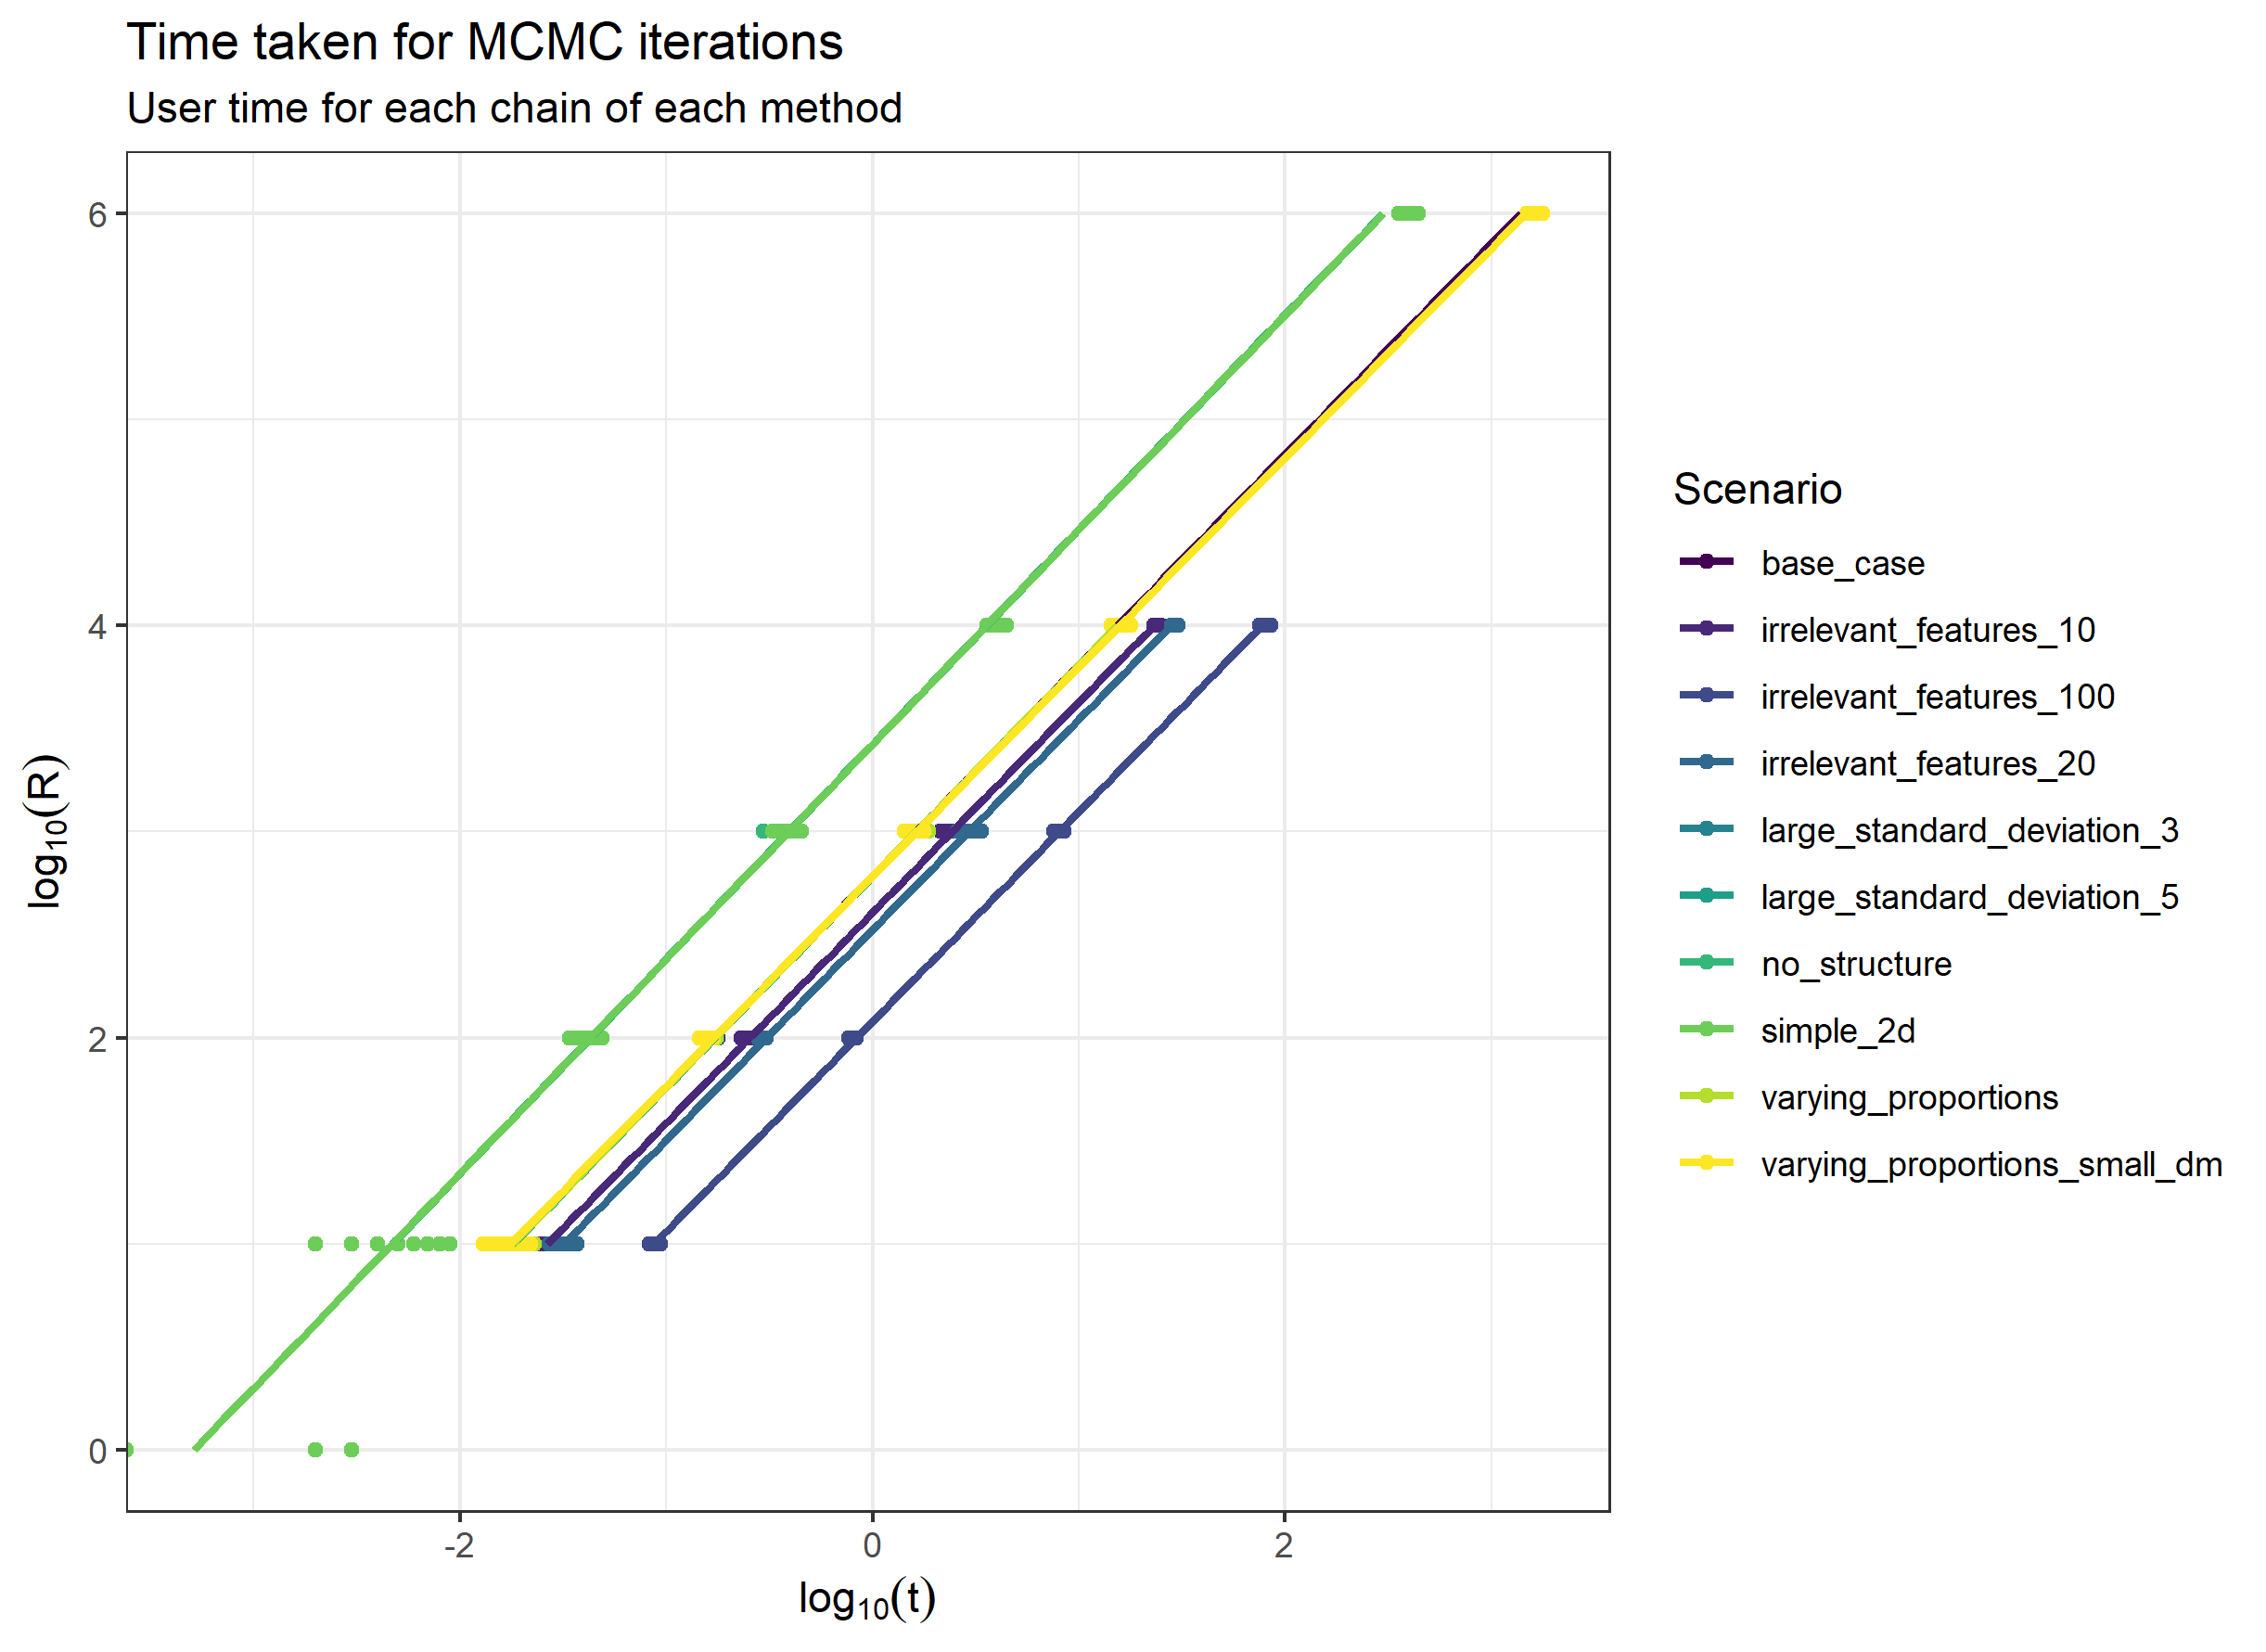
\includegraphics[scale=0.45]{./Images/Simulations/TimeComparison.png}	
	\caption{The time taken for different numbers of iterations of MCMC moves in $\log_{10}(seconds)$. The relationship between chain length, $D$, and the time taken is linear (the slope is approximately 1 on the $\log_{10}$ scale), with a change of intercept for different dimensions. The runtime of each Markov chain was recorded using the terminal command \texttt{time}, measured in milliseconds.}
	\label{fig:timeMCMC}
\end{figure}

Figure \ref{fig:timeMCMC} shows that chain length is directly proportional to the time taken for the chain to run. This means that using an ensemble of shorter chains, as in consensus clustering, can offer large reductions in the time cost of analysis when a parallel environment is available compared to standard Bayesian inference. Even on a laptop of 8 cores running an ensemble of 1,000 chains of length 1,000 will require approximately half as much time as running 10 chains of length 100,000 due to parallelisation, and the potential benefits are far greater when using a large computing cluster.

Additional details of the results for the simulated data can be found in section 4.4 of the Supplementary Material, with an additional 9 scenarios also included.

% If a single iteration requires $t$ seconds, running 100 chains of length 100 using 8 cores takes $1,300t$ compared to 5 chains of 10,000 iterations taking $10,000t$. 

%In the 2D dataset \texttt{mclust} outperforms the Bayesian inference and consensus clustering in terms of the point estimate of the generating structure. 

%\begin{itemize}
%	\item Simple example - Mclust and Bayesian win! We see MCMC exploring well. 
%	\item Small N large P, problems for Bayesian. Separate modes represented in CM, so consensus is finding sensible modes
%	\item Irrelevant 100, many modes, Mclust collapse, similar to above.
%	\item Real data \vspace*{1pt}
%\end{itemize}
%
%Multiple dataset
%\begin{itemize}
%	\item MDI yeast - pretty identical
%	\item Full yeast - Bayesian fails, consensus succeeds
%	\item Cancer - hmmmmmm	\vspace*{1pt}
%\end{itemize}
%
%\begin{figure}[!tpb]%figure1
%\fboxsep=0pt\colorbox{gray}{\begin{minipage}[t]{235pt} \vbox to 100pt{\vfill\hbox to
%235pt{\hfill\fontsize{24pt}{24pt}\selectfont FPO\hfill}\vfill}
%\end{minipage}}
%%\centerline{\includegraphics{fig01.eps}}
%\caption{Caption, caption.}\label{fig:01}
%\end{figure}

%\begin{figure}[!tpb]%figure2
%%\centerline{\includegraphics{fig02.eps}}
%\caption{Caption, caption.}\label{fig:02}
%\end{figure}


%\subsection{Test1}

\subsection{Multi-omics analysis of the cell cycle in budding yeast}
%We include additional results for the integrative analysis in section 5 of the Supplementary Material.

%\subsubsection{Ensemble choice}
We use the stopping rule proposed in \ref{sec:ensembleChoice} to determine our ensemble depth and width. In Figure \ref{fig:ensembleChoice}, we see that the change in the consensus matrices from increasing the ensemble depth and width is diminishing in keeping with results in the simulations. We see no strong improvement after $D=6,000$ and increasing the number of learners from 500 to 1,000 has small effect. We therefore use the largest ensemble available, an ensemble of depth $D=10001$ and width $W=1000$ with a base learner of MDI, with the belief that it is achieving the asymptotic performance described in the simulation results. Some additional evidence for this choice is given in section 5.1 of the Supplementary Material.
% We include 
%the Consensus matrices for this ensemble and those for the combinations of $D = (1001, 5001, 10001)$, $W=(100, 500, 1,000)$ in the three datasets (shown in Figures \ref{fig:timecourseCMs}, \ref{fig:chipchipCMs} and \ref{fig:ppiCMs}) and 
%a plot of the mean squared difference between the consensus matrix for $D=10001$ and $W=1000$ to a range of smaller and shallower ensembles (Figure \ref{fig:ensembleChoice}).

\begin{figure}
	\centering
	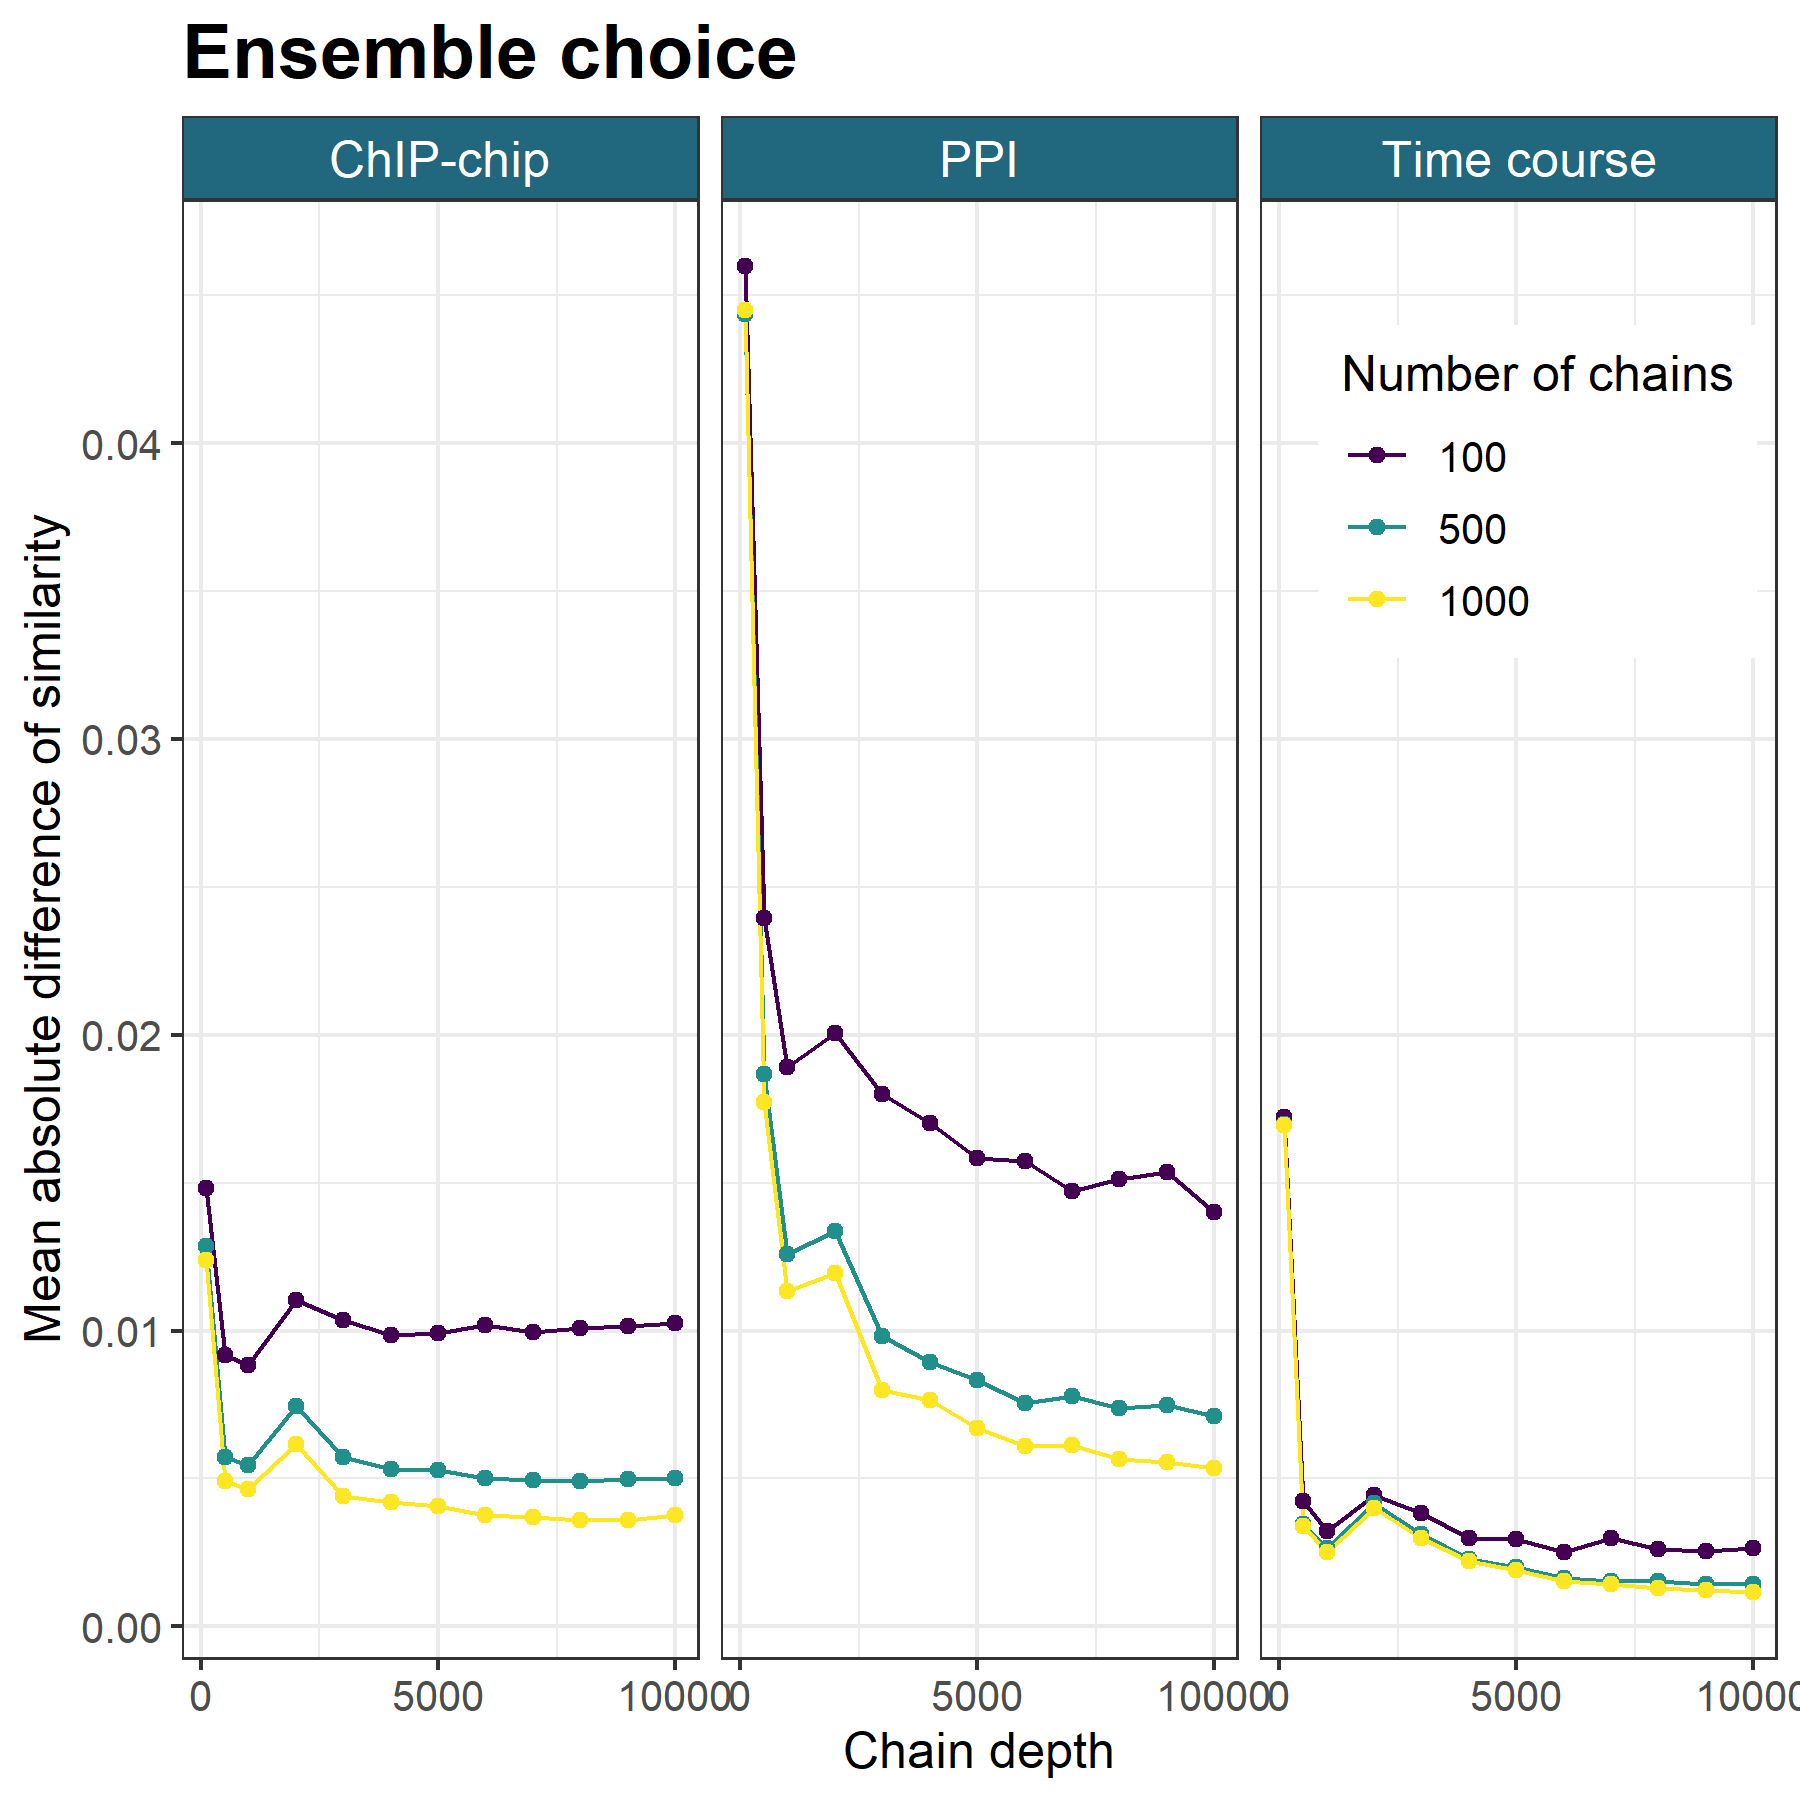
\includegraphics[scale=0.5]{./SupplementaryMaterial/Images/Yeast/EnsembleChoicePlotAlt.png}
	\caption{The mean absolute difference between the sequential Consensus matrices. For a set of chain lengths, $D'=\{d_1, \ldots, d_I\}$ and number of chains, $W'=\{w_1, \ldots, w_J\}$, we take the mean of the absolute difference between the consensus matrix for $(d_i, w_j)$ and $(d_{i-1}, w_{j})$ (here $D'=\{101, 501, 1001, 2001, \ldots, 10001\}$ and $W'=\{100, 500, 1000\}$). 
		%	to the consensus matrix for chain depth 10,001 and 1,000 chains. 
%		We find that increasing $s$ beyond 500 has marginal effect except in the PPI dataset.
		%	where values have stabilised by $W=500$. 
		%	The changes in item coclustering across the ensemble changes very slightly for chains deeper than 5,000 and certainly increasing beyond 8,000 iterations has very little effect.
	}
	\label{fig:ensembleChoice}
\end{figure}
%We decide to stop increasing at $D=10001$ as there is little change between Consensus matrices for increasing chain depth from $D=5001$ to $D=10001$ across the three datasets.
%An example of insufficient depth can be see for $D=1001$ in Figure \ref{fig:ppiCMs}; there is a marked difference in the Consensus matrices between $D=1001$ and $D=5001$. 

%\subsubsection{Integrated clusters}
%We define a gene to be integrated across some set of datasets if the gene has the same label in each of these datasets for at least half of the recorded clustering samples. Integrated genes are those most affected by the integrative aspect of the analysis and therefore we focus upon these. 
We focus upon the genes that tend to have the same cluster label in both the time course and ChIP-chip datasets as being of the most interest for an integrative analysis. 261 genes (nearly half of the genes present) in this pair of datasets have a common label in most chains, whereas only 56 genes have a common label across all three datasets. Thus, we focus upon this pairing of datasets as they appear to share much common signal. More formally, we analyse the clustering structure among genes for which $\hat{P}(c_{nl} = c_{nm}) > 0.5$, where $c_{nl}$ denotes the cluster label of gene $n$ in dataset $l$.
%integrated across the time course  and ChIp-chip datasets as the PPI dataset appears to contribute less to the analysis. 261 genes integrate acorss this pair of datasets (nearly half of the genes present), of which 56 integrate across all three datasets. 
We show the gene expression and regulatory proteins of these genes separated by their cluster in Figure \ref{fig:timepointChIPchipFused}. In this plot we include only the clusters with more than one member and more than half the members having some interacitons in the ChIP-chip data.
%exclude the 15 clusters where more than half of the member genes have no interactions in the ChIP-chip data and any clusters of one gene. 
We find that a small number of transcription factors dominate, with different combinations emerging across the 10 clusters (these and some relevant details are listed in Table 2 of the Supplementary Material). Many of these 10 correspond to transcription factors that are well known to regulate cell cycle expression \citep{simon2001serial}.

\begin{figure*}
	\centering
	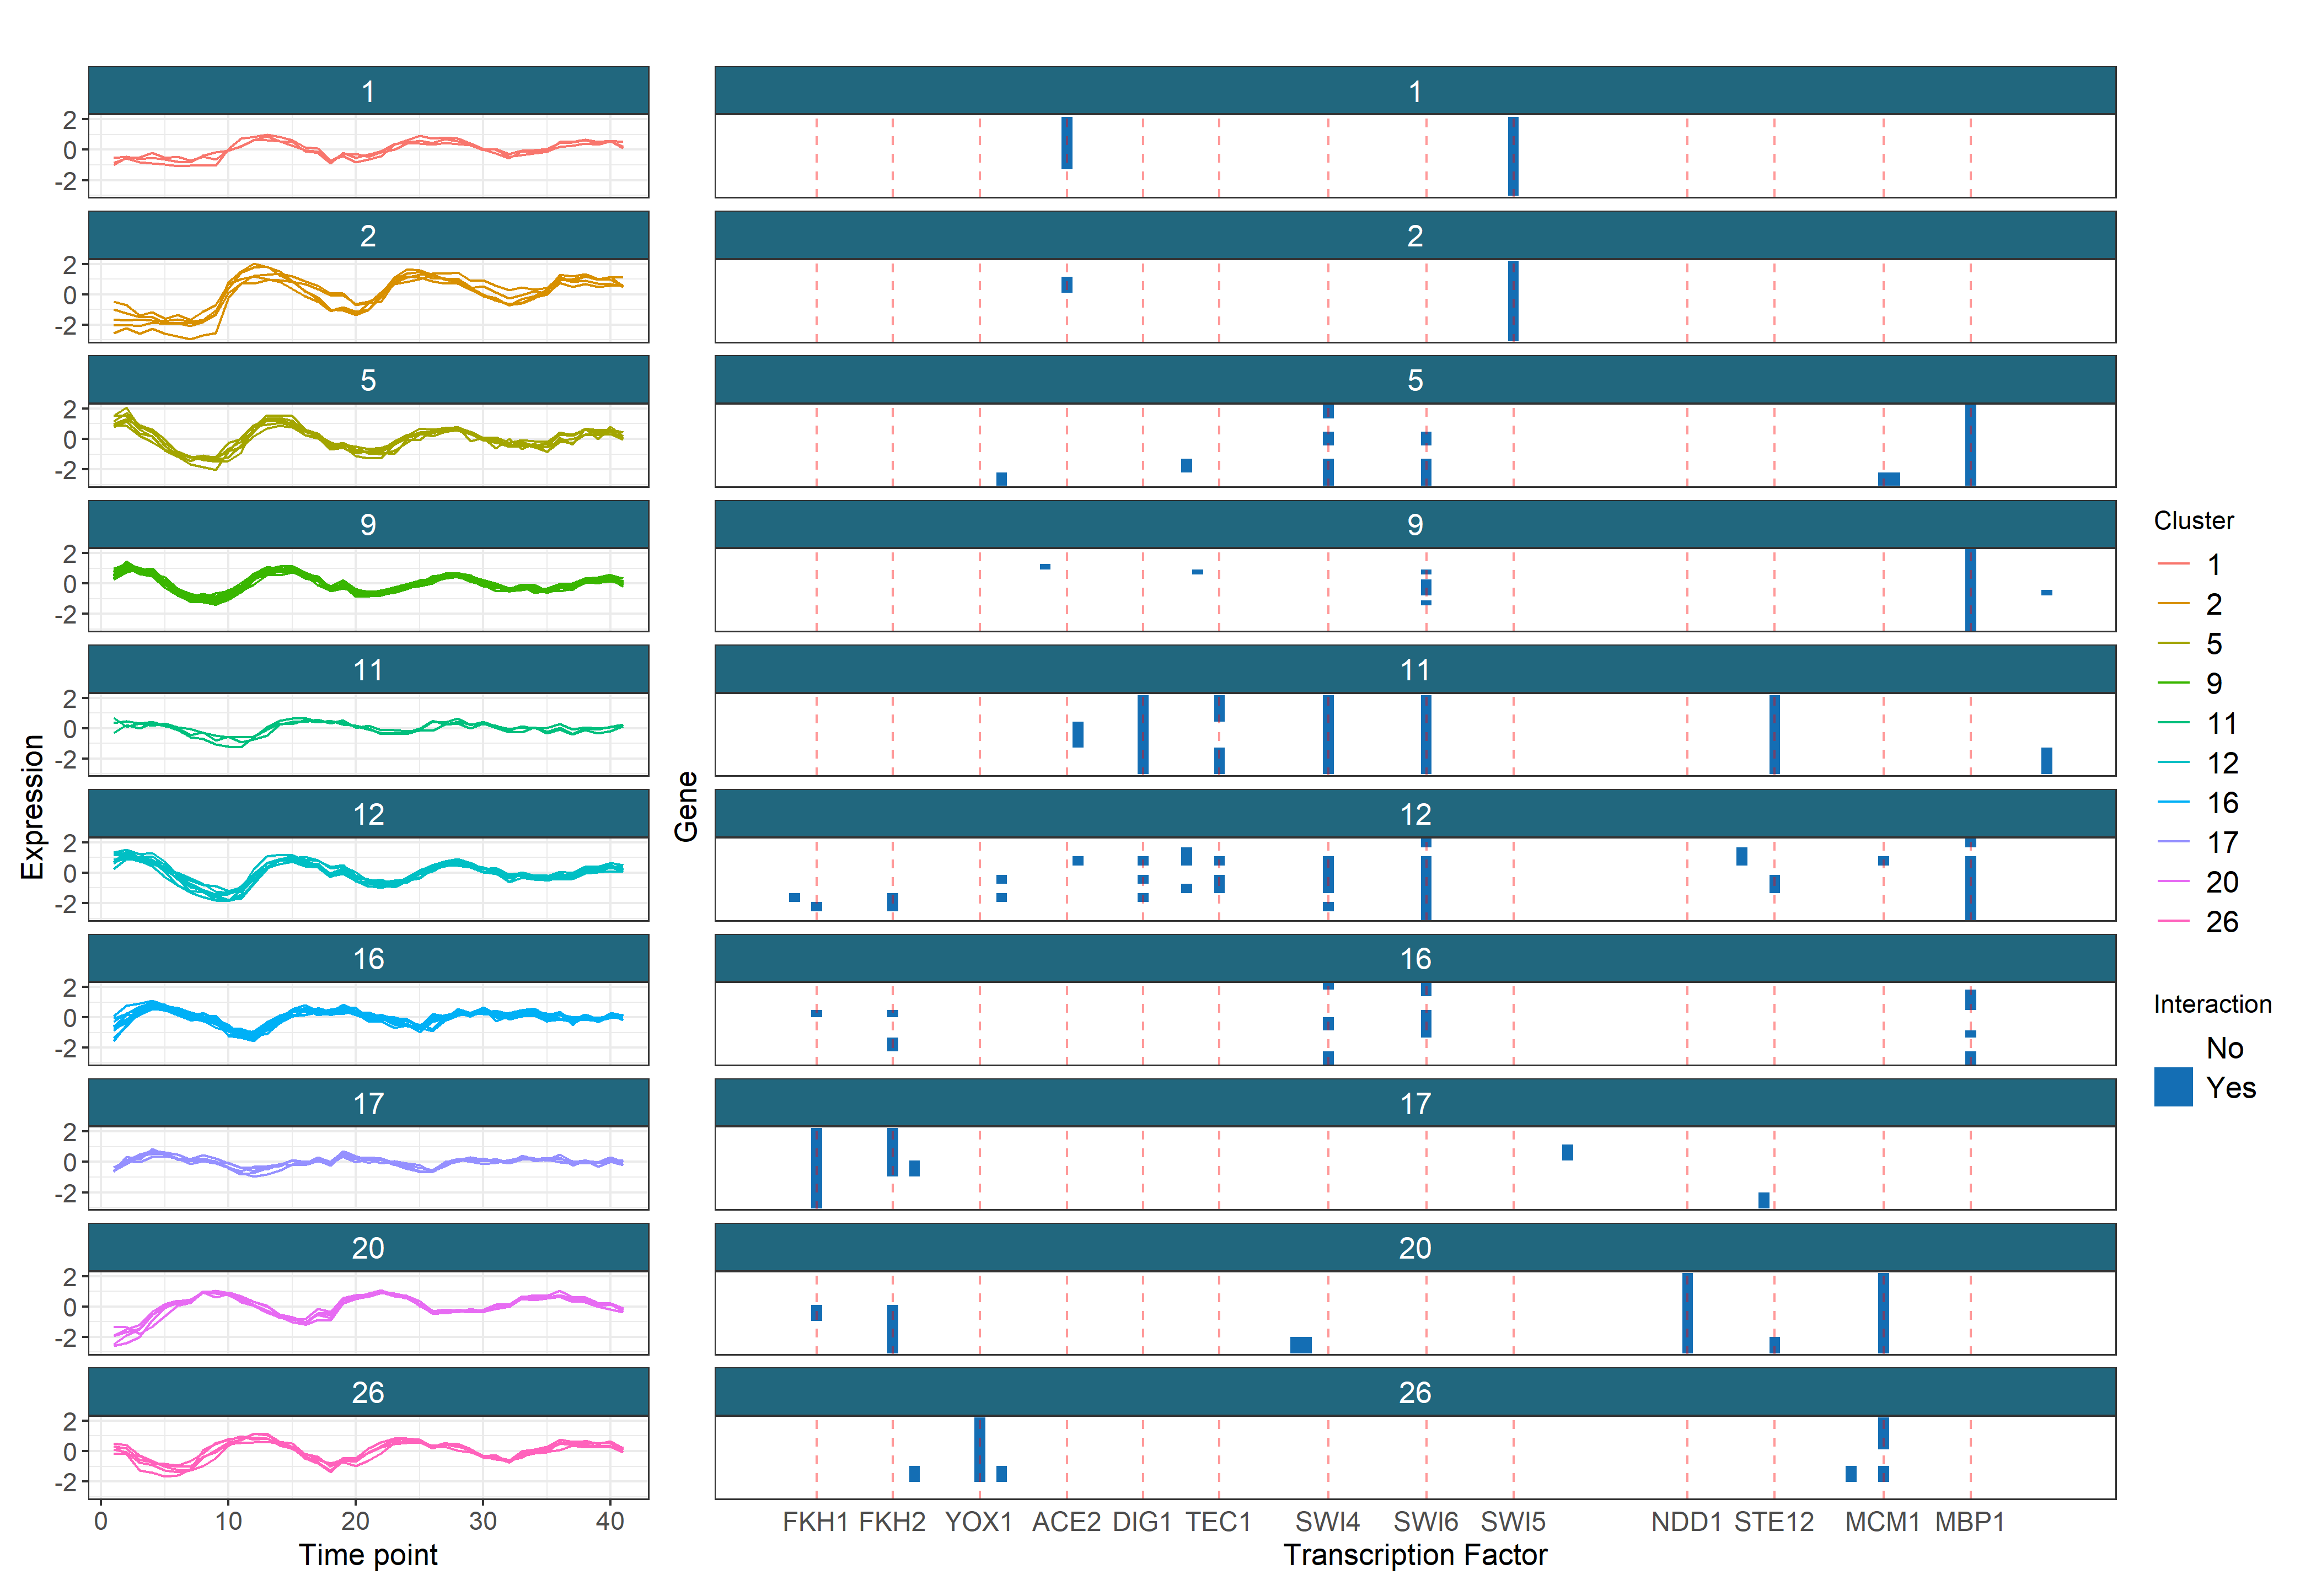
\includegraphics[scale=0.5]{./SupplementaryMaterial/Images/Yeast/timecourseChIPchipFused.png}
	\caption{The genes which tend to have a common label across the time course and ChIP-chip datasets separated out by their clusters. We exclude the clusters with no interactions in the ChIP-chip dataset and include a red line for the transcription factors that dominate the clustering structure in the ChIP-chip dataset. The clusters in the time series data are quite well banded and distinct (having different periods, amplitudes, or both) and in the ChIP-chip data a small number of Transcription factors dominate the clustering structure. The clusters have tight, unique signatures in the time course dataset and tend to be defined by a small number of well-studied transcription factors in the ChIP-chip dataset.}
	\label{fig:timepointChIPchipFused}
\end{figure*}

As an example, we briefly analyse clusters 9 and 16 in greater depth. Cluster 9 has strong association with MBP1 and some interactions with SWI6, as can be seen in Figure \ref{fig:timepointChIPchipFused}. The Mbp1-Swi6p complex, MBF, is associated with DNA replication \citep{iyer2001genomic}. The first time point, 0 minutes, in the time course data is at the START checkpoint, or the G1/S transition. The members of cluster 9 begin highly expressed at this point before quickly dropping in expression (in the first of the 3 cell cycles). This suggests that many transcripts are produced immediately in advance of S-phase, and thus are required for the first stages of DNA synthesis. We used the \texttt{org.Sc.sgd.db} \citep{carlson2014org} package to find gene descriptions (which are included in Table 3 of the Supplemenatry Material). These descriptions support this hypothesis, as we find that many of the genes in cluster 9 are associated with DNA replication, repair and/or recombination. Members of the replication checkpoint, TOF1, MRC1 and RAD53 \citep{bando2009csm3, lao2018yeast} also emerge in the cluster as do some members of the cohesin complex. Cohesin is associated with sister chromatid cohesion, which is established during the DNA synthesis phase of the cell cycle \citep{toth1999yeast}, but also contributes to transcription regulation, DNA repair, chromosome condensation, homolog pairing \citep{mehta2013cohesin}, fitting the theme of cluster 9.

Cluster 16 consists of genes whose products form the histones H1, H2A, H2B, H3 and H4 and then has three other members, GAS3, NRM1 and PDS1.  Histones are the chief protein components of chromatin \citep{fischle2003histone} and are important contributors to gene regulation \citep{bannister2011regulation}. They are known to peak in expression in S-phase \citep{granovskaia2010high}, which matches the first peak of this cluster early in the time series. Of the other members, NRM1 is a transcriptional co-repressor of MBF-regulated gene expression acting at the transition from G1 to S-phase \citep{de2006constraining, aligianni2009fission}. Pds1p binds to and inhibits the Esp1 class of sister separating proteins, preventing sister chromatids separation before M phase \citep{ciosk1998esp1, toth1999yeast}. The remaining member, GAS3, is poorly understood. It interacts with SMT3 which regulates chromatid cohesion, chromosome segregation and DNA replication (among other things). Chromatid cohesion ensures the faithful segregation of chromosomes in mitosis and in both meiotic divisions \citep{cooper2009pds1p} and is instantiated in S-phase \citep{toth1999yeast}. These results, along with the very similar expression profile to the histone genes in the time course data, suggest that GAS3 may be involved more directly in DNA replication or chromatid cohesion than is currently believed.

We attempt to perform a similar analysis using traditional Bayesian inference of MDI, but after 36 hours of runtime there is no consistency or convergence across chains. Each chain provides different parameter distributions and clustering estimates, leaving no clear clustering solution. For details of this analysis, see section 5.2 of the Supplementary Material.

%In terms of the number of chains required, we believe this to have stabilised, as there is no obvious change in increasing $W$ from 100 in the time course  and ChiP-chip datasets, and none in any dataset for increasing from $W=500$ to $W=1000$.


%\begin{figure} %[!tpb]
%	\centering
%	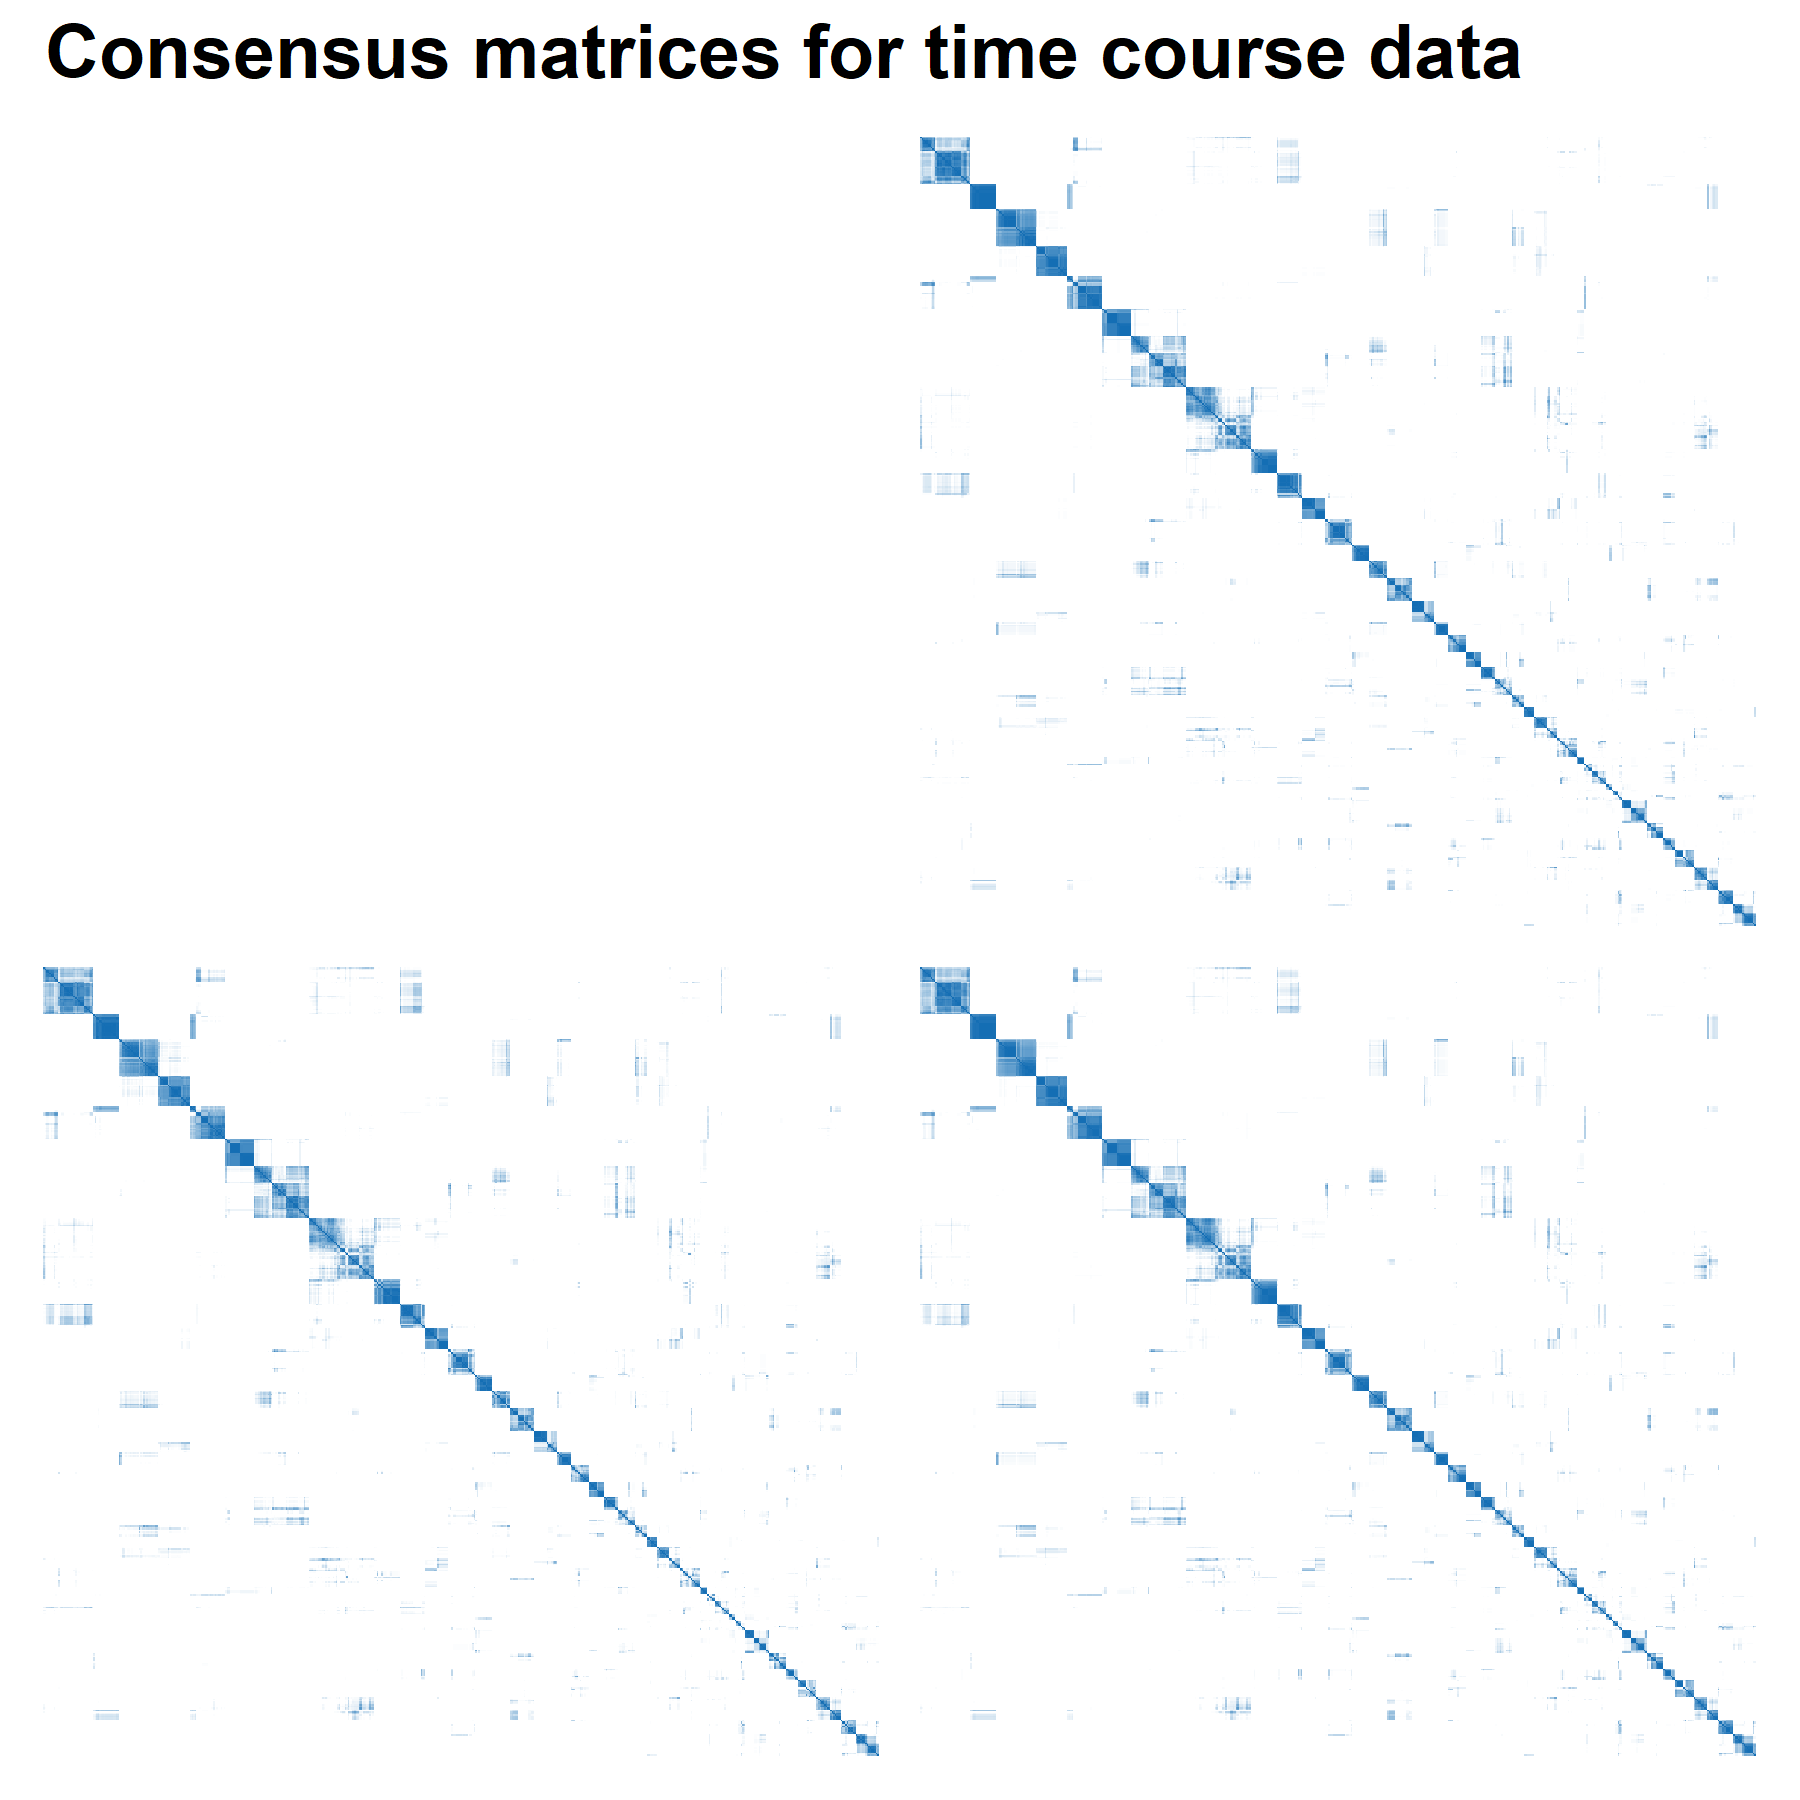
\includegraphics[scale=0.5]{./Images/Yeast/CMs.png}	
%	\caption{The chain length, $D$, and ensemble size $W$, were decided by comparing the consensus matrices for different values of $(D, W)$. Here we show an example for the time course data where $D=100$ in the top row and $D=500$ in the second, and $W=50$ in the first column and $W=100$ in the second. These matrices appear identical, so we stop increasing the chain length or ensemble size.}
%	\label{fig:yeastCMs}
%\end{figure}
%We show the analysis of the clustering inferred for the time course data. Similar analyses for the ChIP-chip and PPI datasets are included in the supplementary materials.
%Convergence of chains was investigated using the Geweke Z-score statistic, with across chain convergence investigated using the Gelman-Rubin diagnostic for the continuous parameters being sampled (here the concentration parameter of the Dirichlet distribution on the component weights and the $\phi_{ij}$ parameters from the MDI model). 
%
%\begin{figure} %[!tpb]
%\centering
%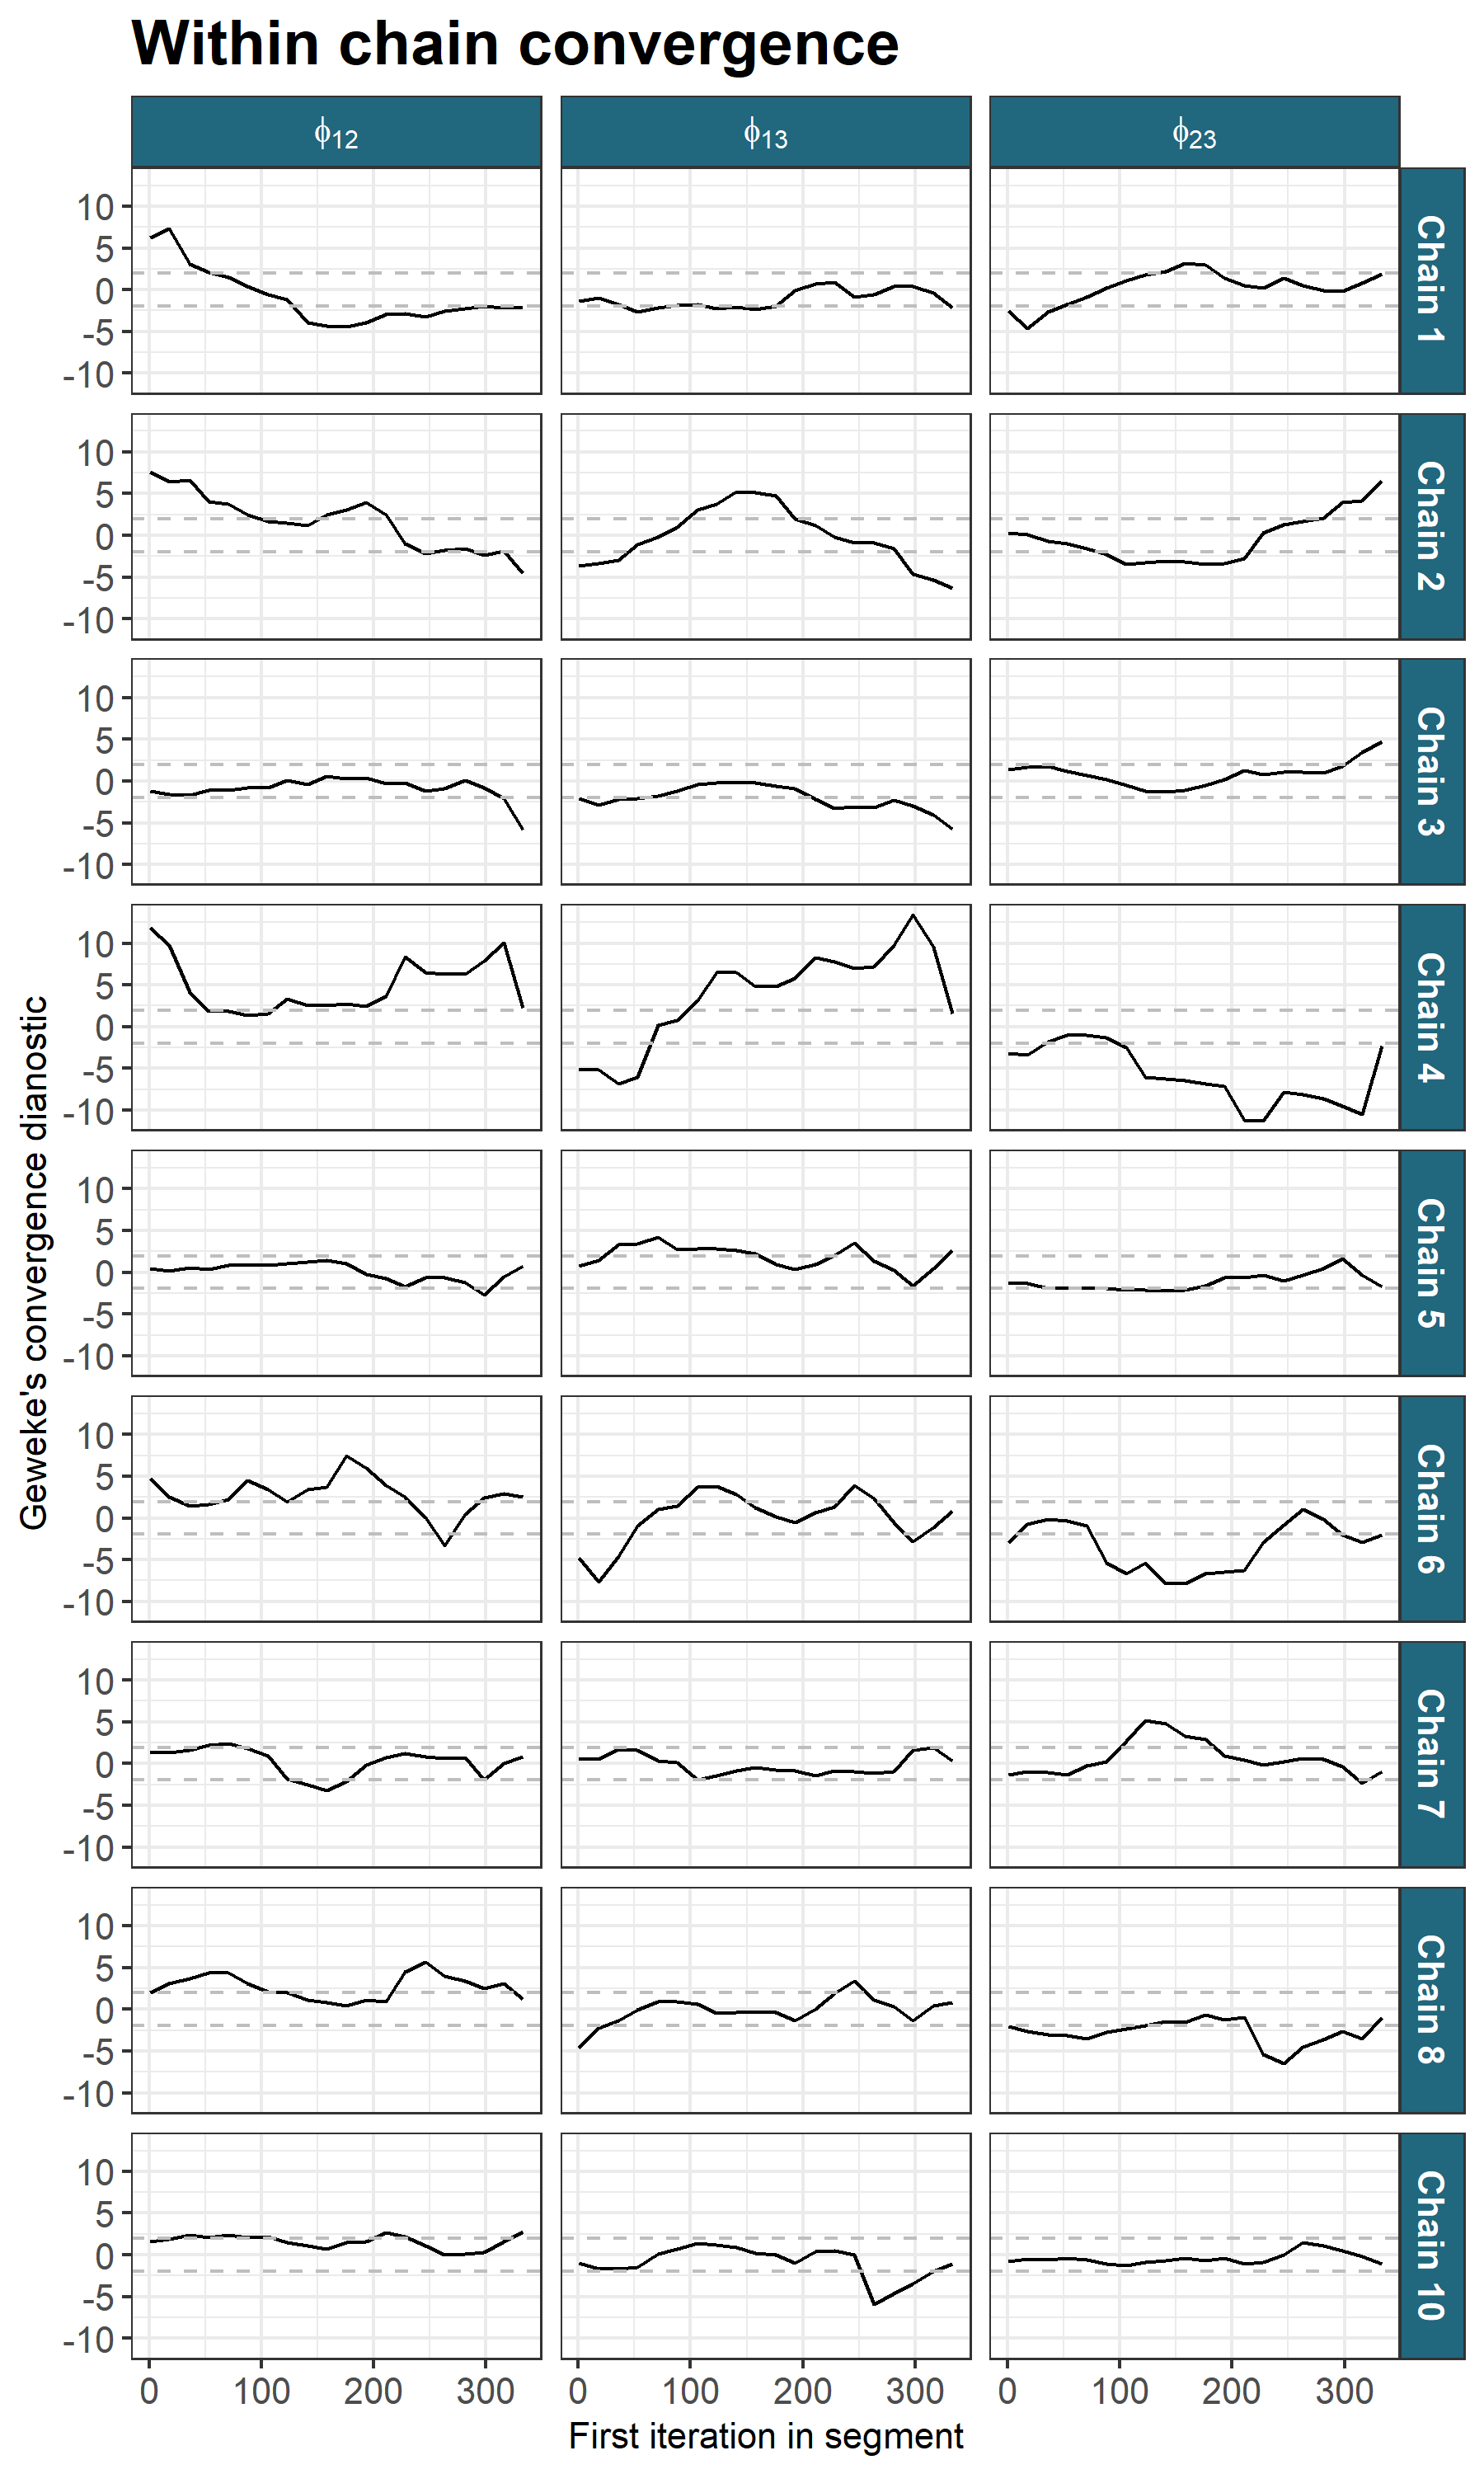
\includegraphics[scale=0.5]{./Images/Yeast/gelmanPlot.png}	
%\caption{The $\hat{R}$ values remain sufficiently far from 0 that the chains should not be considered converged.}
%\label{fig:yeastCMs}
%\end{figure}

%We performed a Gene Ontology (GO) enrichment analysis of our inferred clusters using the \texttt{Bioconductor} packages \texttt{biomaRt} \citep{durinck2005biomart, durinck2009mapping} and \texttt{clusterProfiler} \citep{yu2012clusterProfiler}. The long chains disagree with each other, with each chain having some unique GO terms. Chain 1 appears to be furthest removed from the other 3, with a larger number of terms not found in the other chains associated with some clusters, and also missing some terms common to the other 3. Consensus clustering finds clusters enriched for all the terms common to the long chains as well as finding several clsuters associated with terms not found by any chain. 
%\begin{figure} %[!tpb]
%	\centering
%	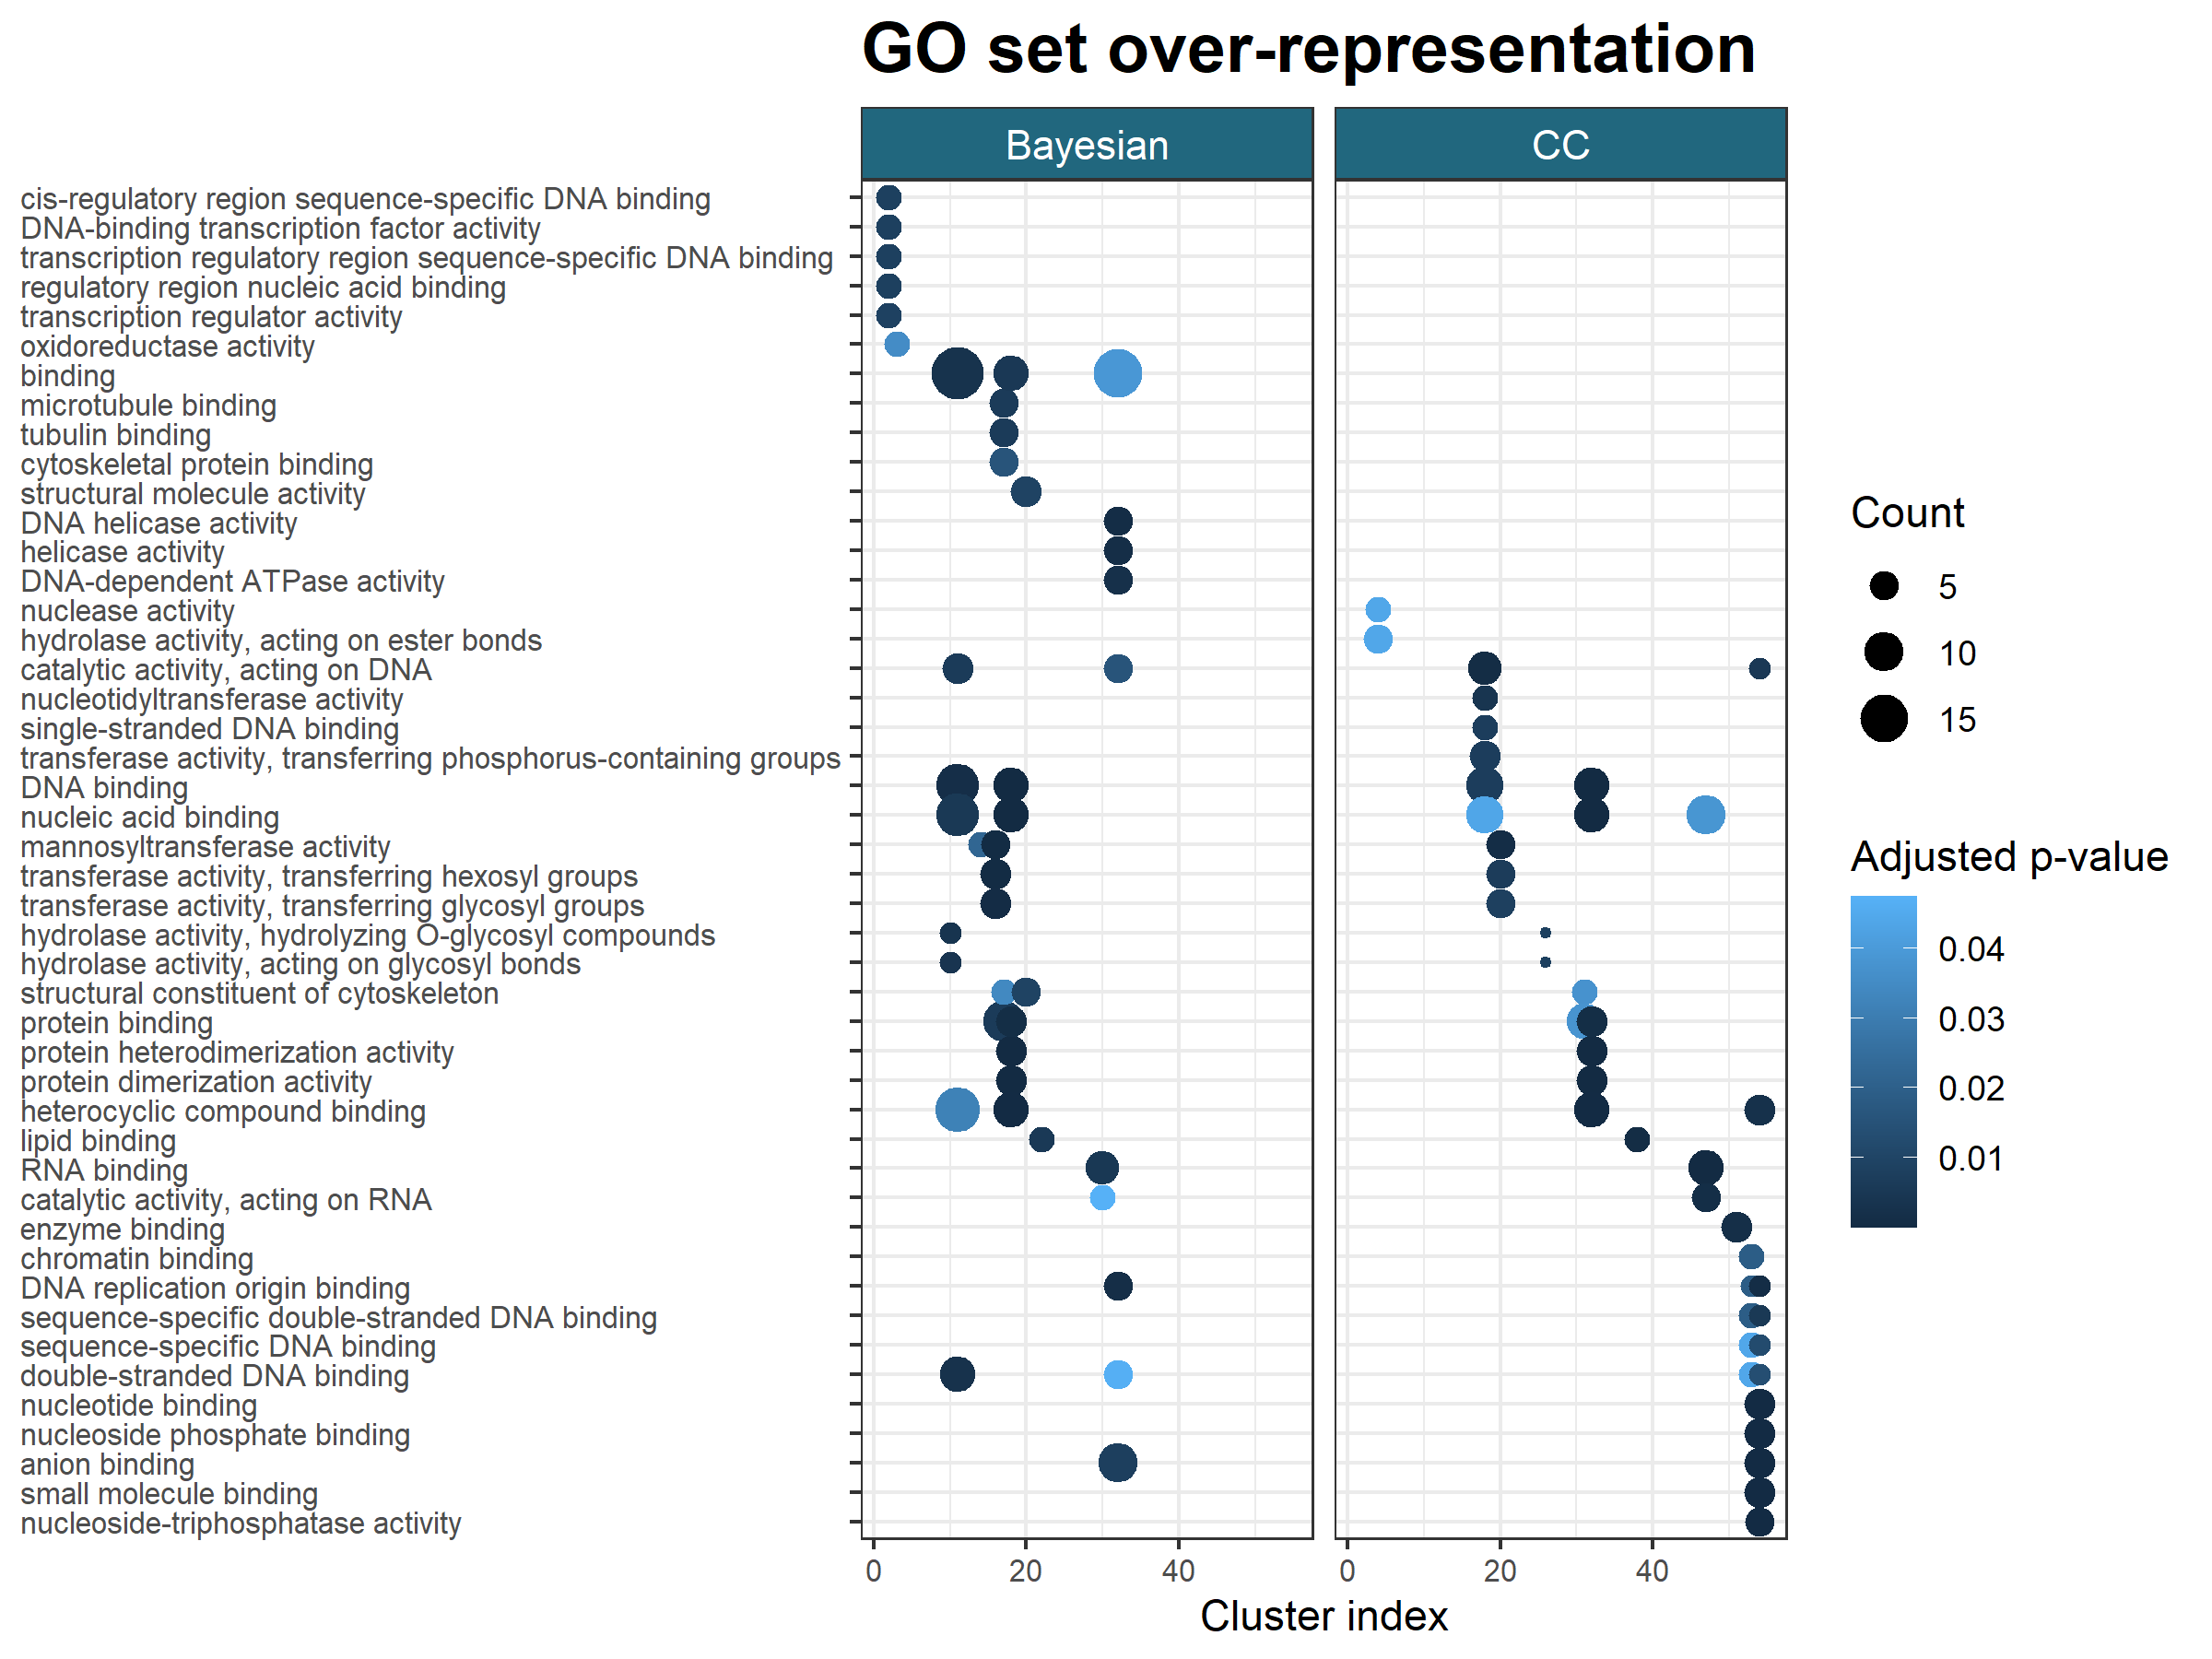
\includegraphics[scale = 0.6]{./Images/Yeast/GOoverRepresentation.png}	
%	\caption{GO term over representation in the clusters using the \emph{molecular function} ontology.}
%	\label{fig:yeastGO}
%\end{figure}

%\begin{figure*} %[!tpb]
%	\centering
%	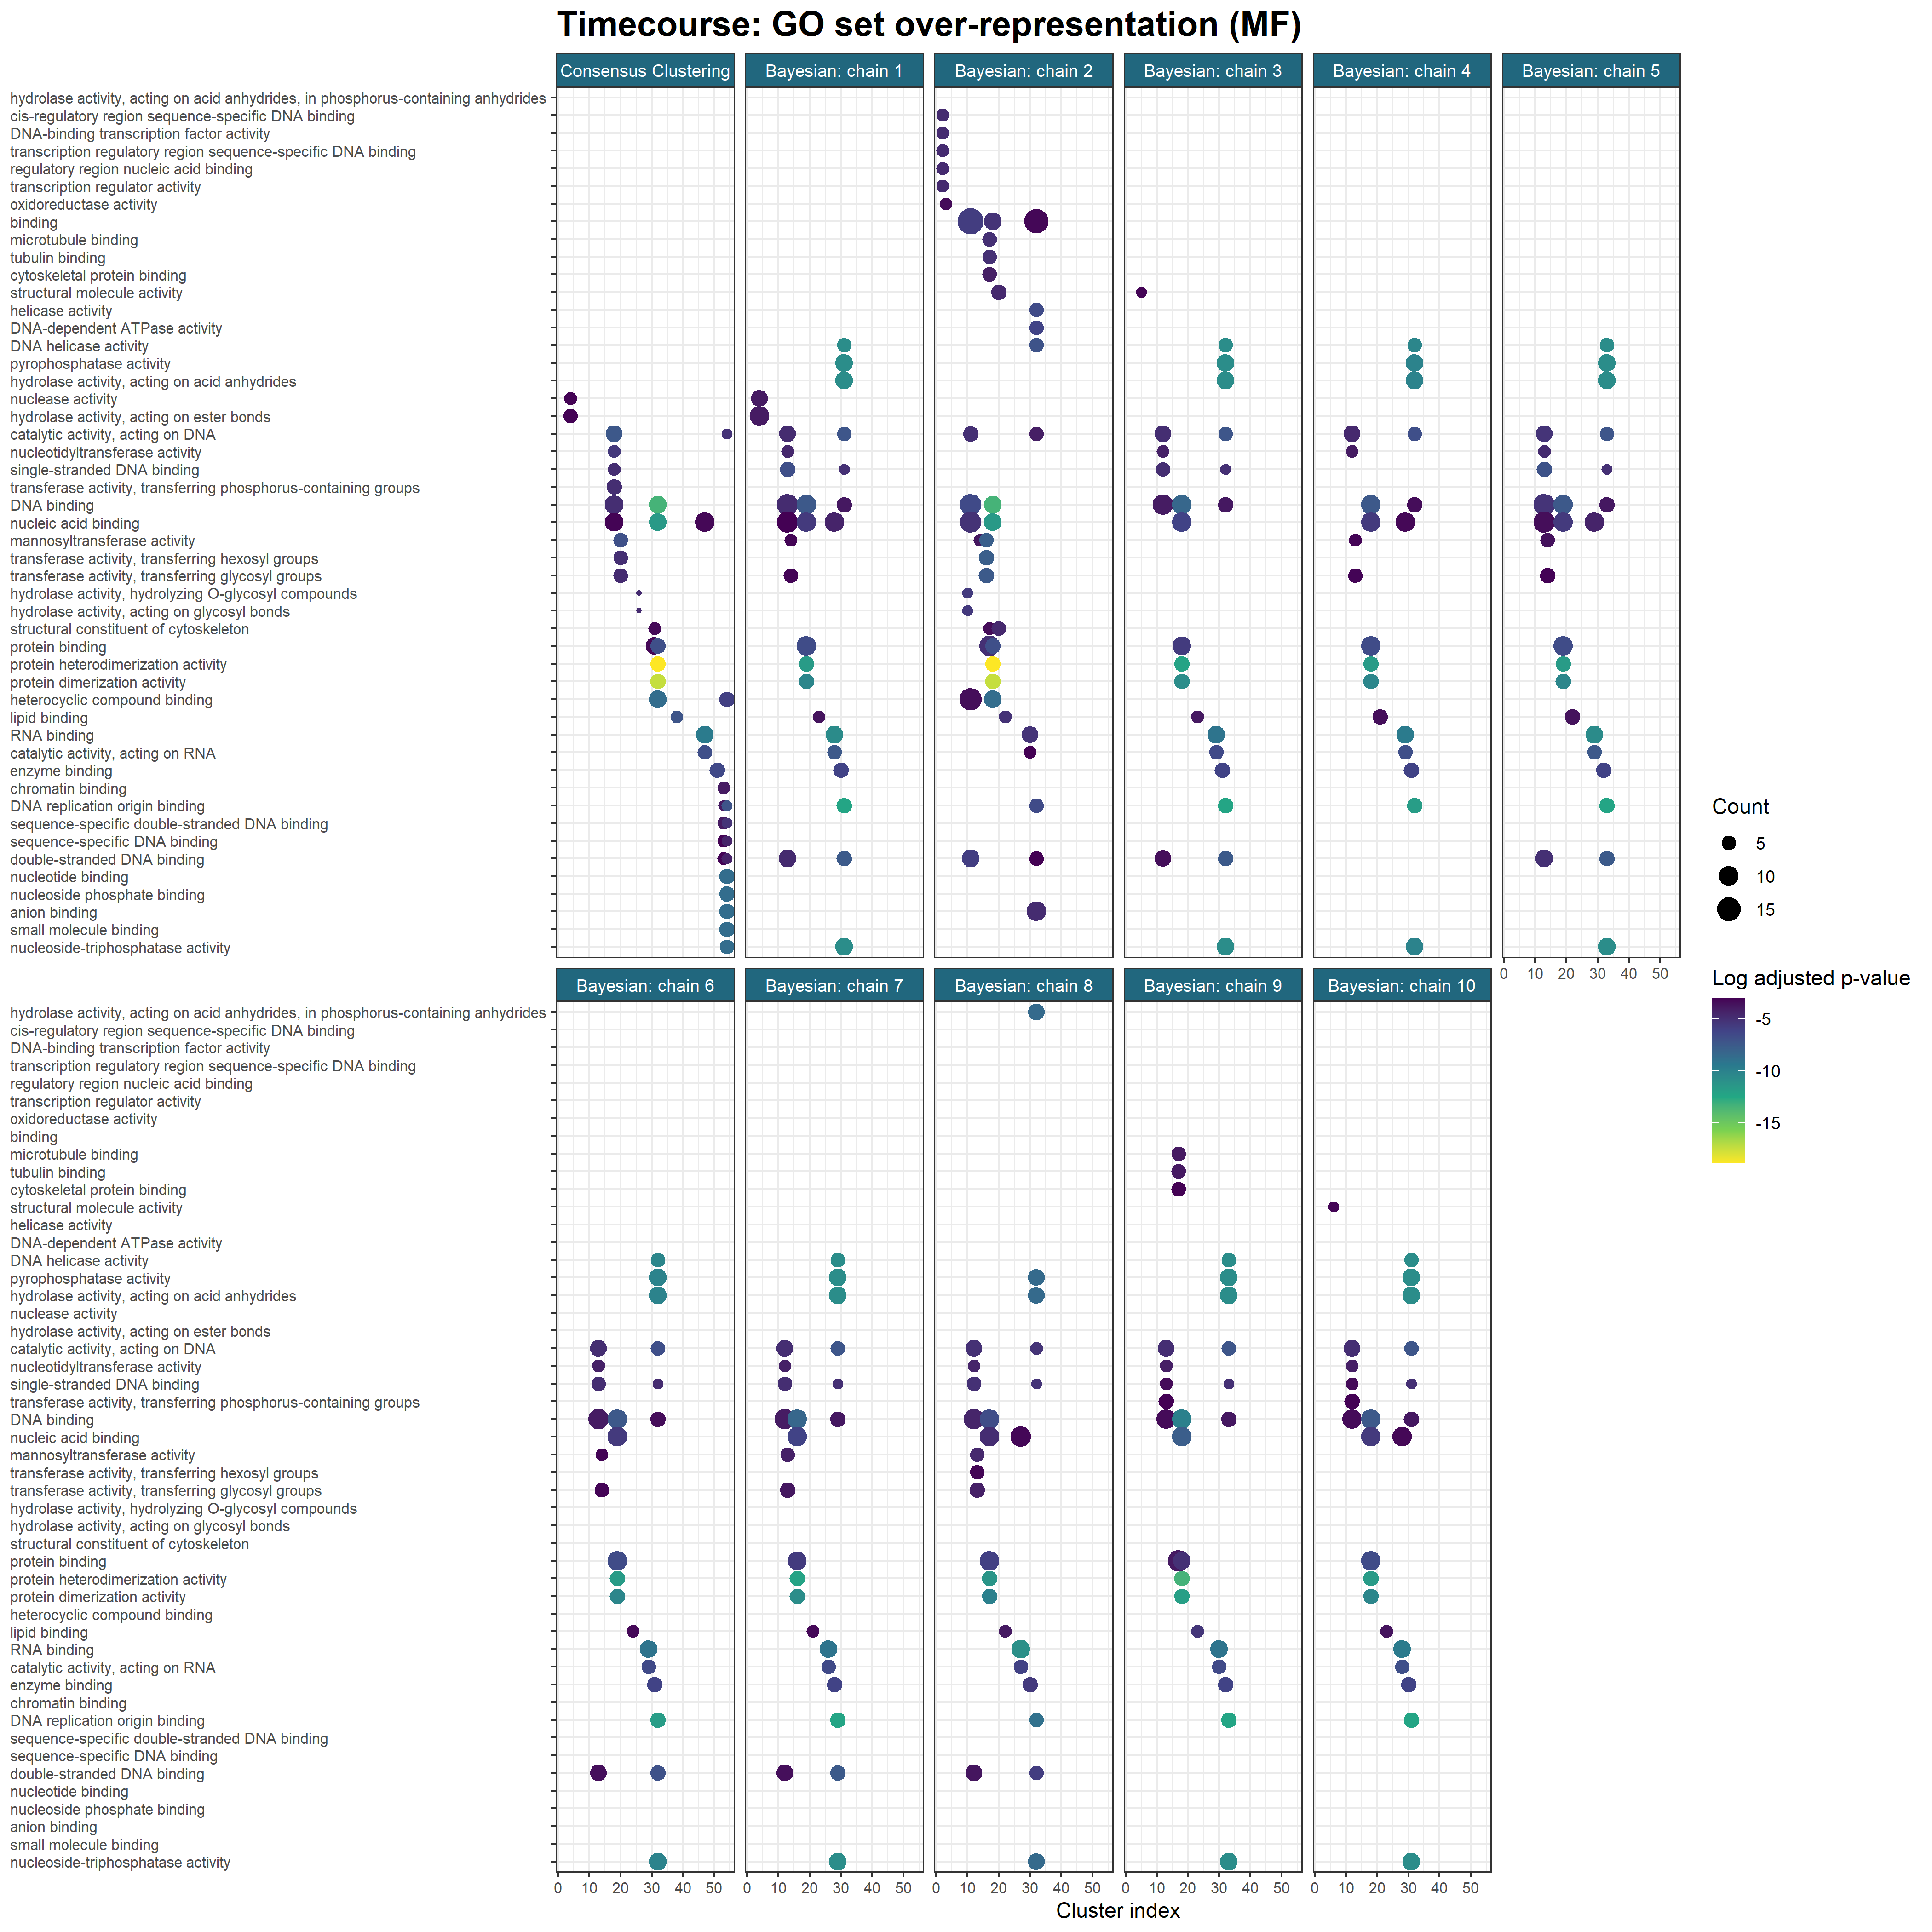
\includegraphics[scale=0.5]{./Images/Yeast/Timecourse/GOoverRepresentationComparisonMF.png}
%	\caption{GO term over representation in the clusters using the \emph{molecular function} ontology. The enriched GO terms disagree across long chains. Consensus clustering finds many of the same functions, with some new functions added. The predicted clustering does lose some of the GO terms not present in all modes.}
%	\label{fig:yeastGOchains}
%\end{figure*}

\section{Discussion}
Our proposed method has demonstrated good performance on simulation studies, uncovering generating structure and approximating Bayesian inference when the Markov chain is exploring the full support of the posterior. However, we have shown that if a finite Markov chain fails to describe the full posterior and is itself only approximating Bayesian inference, our method has better ability to represent several modes in the data than individual chains and thus offers a more consistent and reproducible analysis. Furthermore, consensus clustering is significantly faster in a parallel environment than inference using individual chains, while retaining the ability to robustly infer $K$, the number of occupied components present. 

Based upon the simulations we proposed a method of assessing ensemble stability and deciding upon ensemble size. We then performed an integrative analysis of yeast cell cycle data using MDI, an extension of Bayesian mixture models that jointly models multiple datasets. We sidestep convergence issues and decrease the computational cost of such a large model by applying consensus clustering to it, showing the flexibility of consensus clustering and its applicability to any clustering method that uses MCMC methods to sample partitions. We used our proposed stopping rule to decide upon our ensemble size and uncovered many genes with shared signal across several datasets. We then explored the biological meaning of some of the uncovered clusters, using data external to the analysis, finding sensible results as well as signal for possibly novel biology. 

The results of our simulations and the multi-omics analysis show that consensus clustering can be used in a broad context, being applicable to any MCMC based clustering method, not solely to mixture models. It offers computational gains and greater applicability to these methods as a result and, attractively, it can be applied to existing implementations, unlike improvements to the underlying MCMC methods or alternative methods for Bayesian inference such as VI which would require re-writing software. However, consensus clustering does lose the theoretical framework of true Bayesian inference. We attempt to mitigate this with our assessment of stability in the ensemble, but this diagnosis is heuristic and subjective, and while there is empirical evidence for its success, it lacks the formal results for the tests of model convergence for Bayesian inference.

We expect that researchers interested in applying some of the Bayesian integrative clustering models such as MDI and Clusternomics \citep{gabasova2017clusternomics} will be enabled to do so, as consensus clustering overcomes some of the unwieldiness of these large, joint models. More generally, we expect that our method will be useful to researchers performing cluster analysis of high-dimensional data where the runtime of MCMC methods becomes too onerous and multi-modality is more likely to be present.

%We expect that consensus clustering could be applied with similar success to other extensions of Bayesian mixture models such as Clusternomics \citep{gabasova2017clusternomics}.



%Could the early stopping of the MCMC algorithm be a form of regularisation, making the model more robust to misspecification? In line with early stopping from Deep Learning (see \citealp{morgan1990generalization}), regularisation and misspecification idea from \cite{miller2018robust, cai2020finite}.


%%%%%%%%%%%%%%%%%%%%%%%%%%%%%%%%%%%%%%%%%%%%%%%%%%%%%%%%%%%%%%%%%%%%%%%%%%%%%%%%%%%%%
%
%     please remove the " % " symbol from \centerline{\includegraphics{fig01.eps}}
%     as it may ignore the figures.
%
%%%%%%%%%%%%%%%%%%%%%%%%%%%%%%%%%%%%%%%%%%%%%%%%%%%%%%%%%%%%%%%%%%%%%%%%%%%%%%%%%%%%%%






%\section{Conclusion}
%
%(Table~\ref{Tab:01}) Text Text Text Text Text Text  Text Text Text
%
%\begin{enumerate}
%\item this is item, use enumerate
%\item this is item, use enumerate
%\item this is item, use enumerate
%\end{enumerate}
%
%
%
%
%\section*{Acknowledgements}
%
%Text Text Text Text Text Text  Text Text. nt to know about  text
%text text text\vspace*{-12pt}

\section*{Funding}
SC is supported by an UKRI Studentship via the MRC https://mrc.ukri.org/ (MC UU 00002/4). PK is supported by the MRC (MC UU 00002/13). CW is supported by the Wellcome Trust https://wellcome.ac.uk/ (WT107881) and the MRC (MC UU 00002/4). This research was funded in whole, or in part, by the Wellcome Trust [Grant number WT107881]. For the purpose of open access, the author has applied a CC BY public copyright licence to any Author Accepted Manuscript version arising from this submission. The funders had no role in study design, data collection and analysis, decision to publish, or preparation of the manuscript.
\vspace*{-12pt}

\bibliographystyle{natbib}
%\bibliographystyle{achemnat}
%\bibliographystyle{plainnat}
%\bibliographystyle{abbrv}
%\bibliographystyle{bioinformatics}
%
%\bibliographystyle{plain}
%
%\bibliography{document}
\bibliography{CCbib}  

% \begin{thebibliography}{}

% \bibitem[Bofelli {\it et~al}., 2000]{Boffelli03}
% Bofelli,F., Name2, Name3 (2003) Article title, {\it Journal Name}, {\bf 199}, 133-154.

% \bibitem[Bag {\it et~al}., 2001]{Bag01}
% Bag,M., Name2, Name3 (2001) Article title, {\it Journal Name}, {\bf 99}, 33-54.

% \bibitem[Yoo \textit{et~al}., 2003]{Yoo03}
% Yoo,M.S. \textit{et~al}. (2003) Oxidative stress regulated genes
% in nigral dopaminergic neurnol cell: correlation with the known
% pathology in Parkinson's disease. \textit{Brain Res. Mol. Brain
% Res.}, \textbf{110}(Suppl. 1), 76--84.

% \bibitem[Lehmann, 1986]{Leh86}
% Lehmann,E.L. (1986) Chapter title. \textit{Book Title}. Vol.~1, 2nd edn. Springer-Verlag, New York.

% \bibitem[Crenshaw and Jones, 2003]{Cre03}
% Crenshaw, B.,III, and Jones, W.B.,Jr (2003) The future of clinical
% cancer management: one tumor, one chip. \textit{Bioinformatics},
% doi:10.1093/bioinformatics/btn000.

% \bibitem[Auhtor \textit{et~al}. (2000)]{Aut00}
% Auhtor,A.B. \textit{et~al}. (2000) Chapter title. In Smith, A.C.
% (ed.), \textit{Book Title}, 2nd edn. Publisher, Location, Vol. 1, pp.
% ???--???.

% \bibitem[Bardet, 1920]{Bar20}
% Bardet, G. (1920) Sur un syndrome d'obesite infantile avec
% polydactylie et retinite pigmentaire (contribution a l'etude des
% formes cliniques de l'obesite hypophysaire). PhD Thesis, name of
% institution, Paris, France.

% \end{thebibliography}
\end{document}

\end{equation}